%TODO: 
% ARREGLAR FUNCION EXPONENCIAL CRECIENTE Y DECRECIENTE, DEPENDE DEL CONTEXTO
% MULETILLAS: ADEMAS, CABE DESTACAR, es decir

\documentclass{article}
\usepackage[utf8]{inputenc}
\usepackage[spanish]{babel}
\usepackage[draft]{graphicx}
\usepackage{graphics, float, fancyhdr, titling, caption, subcaption}
\usepackage{listings}
\usepackage[a4paper, total={6in, 9.5in}]{geometry}
\usepackage{fancyhdr}
\usepackage{xcolor}
\usepackage{hyperref}   %para que funcione addcontentsline debe ser la ultima que se cargue

\color{red}

%\setcounter{secnumdepth}{-2}       %Poner solo esto si no se quieren numero delante de las secciones y niveles inferiores.

\renewcommand{\footrulewidth}{0.4pt}
\title{

\includegraphics[width=1.75in]{imagenes/UGR-Logo.png} \\
\vspace*{1in}
\textbf{Memoria de la práctica 2} \\
Animación por Ordenador \\
\vspace*{0.5in}}
\author{Andrés Merlo Trujillo \\
andresmerlo@correo.ugr.es \\
77147239H \\ 
\vspace*{0.5in} \\
E.T.S. de Ingenierías Informática y de Telecomunicación \\
\textbf{Universidad de Granada}} \date{\today}

\hypersetup{
    colorlinks=true,
    linkcolor=black,
    citecolor=black
}

\renewcommand\maketitlehooka{\null\mbox{}\vfill}
\renewcommand\maketitlehookd{\vfill\null}

\begin{document}
\begin{titlingpage}
\maketitle
\end{titlingpage}

\tableofcontents

\newpage

\pagestyle{fancy}   %a partir de comienza el header (se salta el indice y portada)
\fancyhead[L]{Andrés Merlo Trujillo}
\fancyhead[R]{Animación por Ordenador}
%\section{Ejercicio 1}
%\begin{figure}[H]
%    \centering
%    \includegraphics[width=\textwidth]{imagenes/passwdfile.png}
%    \vspace{10pt}
%    \footnotesize{Fuente: https://...}
%\end{figure}

% \begin{figure}[H]
%     \centering 
% 	\begin{subfigure}[H]{0.48\textwidth}
% 	    \centering
% 	    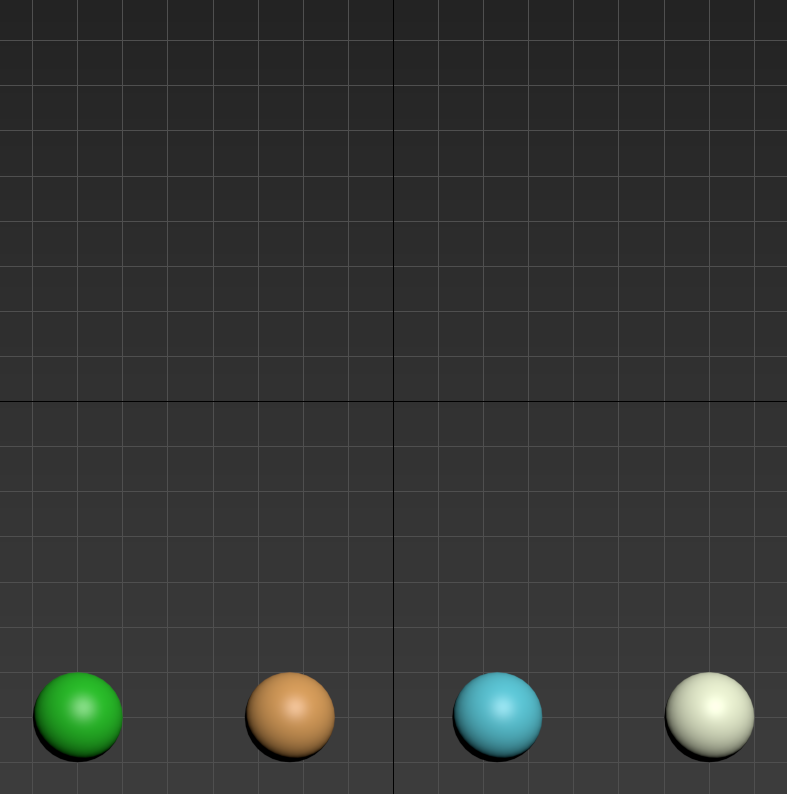
\includegraphics[width=\textwidth]{imagenes/Ejercicio 1/keyframes/0.png}
%         \caption{Pelotas en el instante 0.}
%     \end{subfigure}
%     \hfill
% 	\begin{subfigure}[H]{0.48\textwidth}
% 	    \centering
% 	    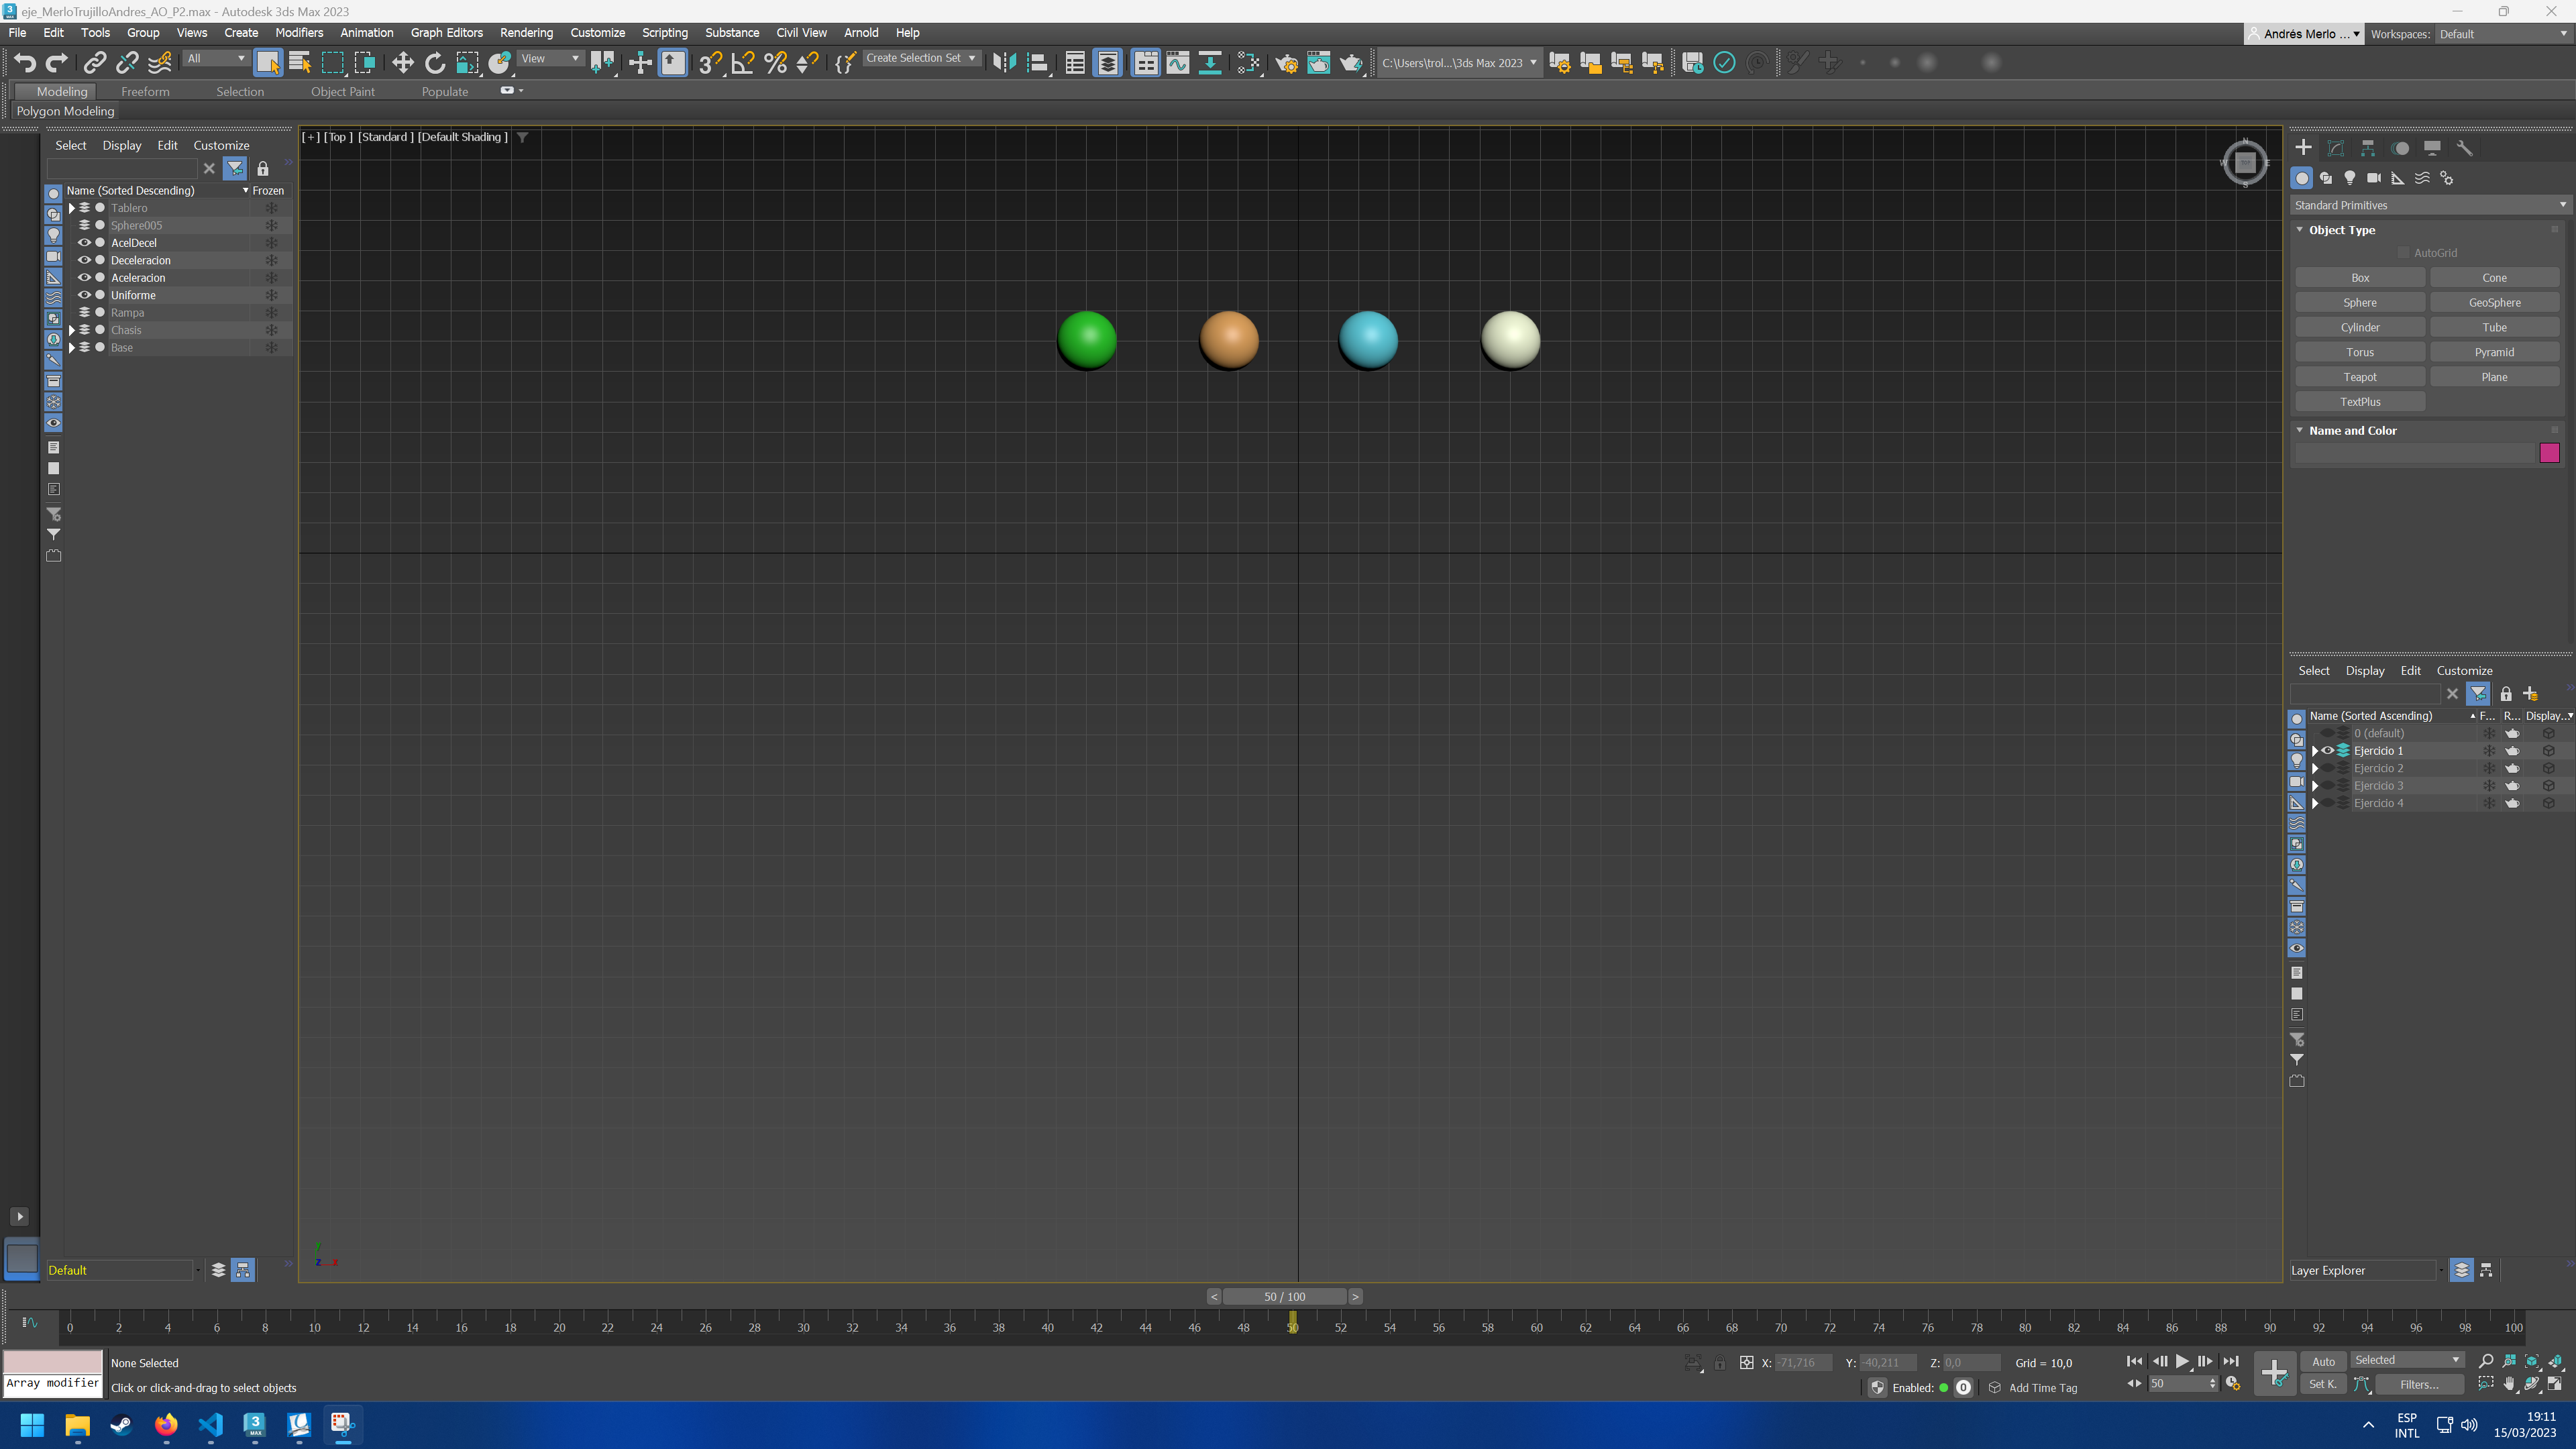
\includegraphics[width=\textwidth]{imagenes/Ejercicio 1/keyframes/50.png}
%         \caption{Pelotas en el instante 50.}
%     \end{subfigure}    
% \end{figure}
\section{Ejercicio 1 - Pelota rodando}
{\color{green}
En este ejercicio se pide implementar la animación de cuatro pelotas (o de una sola pelota haciendo una trayectoria cuadrada) que parten desde un punto A y llegan al mismo tiempo a otro punto B. Se deben usar curvas para crear las animaciones diferentes.

\bigskip

Cabe destacar que los \textit{keyframes} para todas las pelotas son exactamente los mismos, pero cambiando la forma de la función de interpolación para que sus movimientos sean distintos. Entonces, los \textit{keyframes} son los siguientes:

\begin{enumerate}
    \item \textbf{Instante 0:} Posición inicial en el punto A.
    \item \textbf{Instante 50:} Posición final en el punto B.
\end{enumerate}

Y de manera gráfica, los \textit{keyframes} son:

%fotos de una bola nada mas con los keyframes
\begin{figure}[H]
    \centering 
	\begin{subfigure}[H]{0.48\textwidth}
	    \centering
	    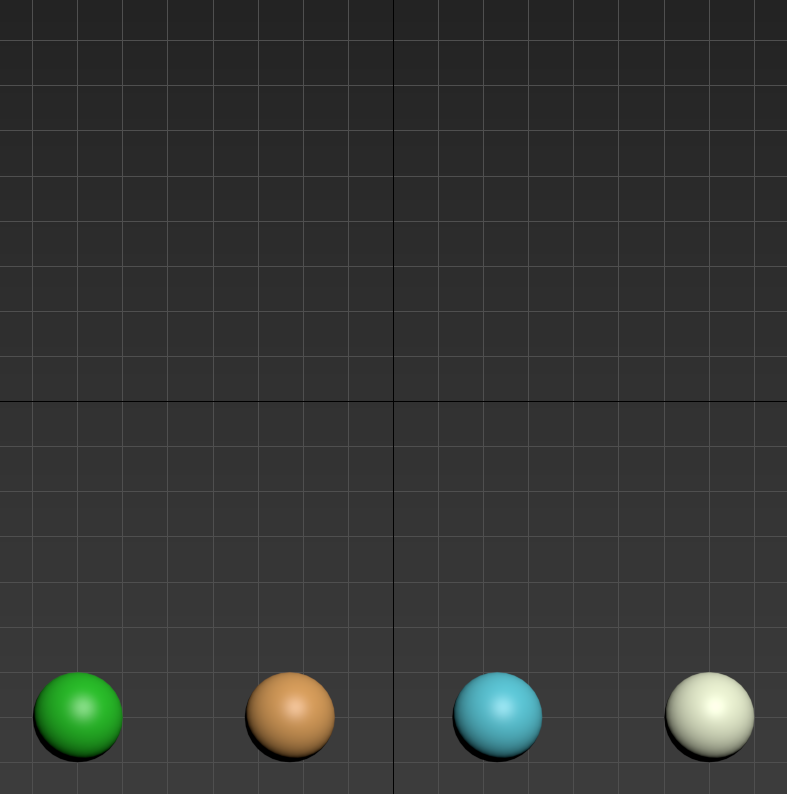
\includegraphics[width=\textwidth]{imagenes/Ejercicio 1/keyframes/0.png}
        \caption{Pelotas en el instante 0.}
    \end{subfigure}
    \hfill
	\begin{subfigure}[H]{0.48\textwidth}
	    \centering
	    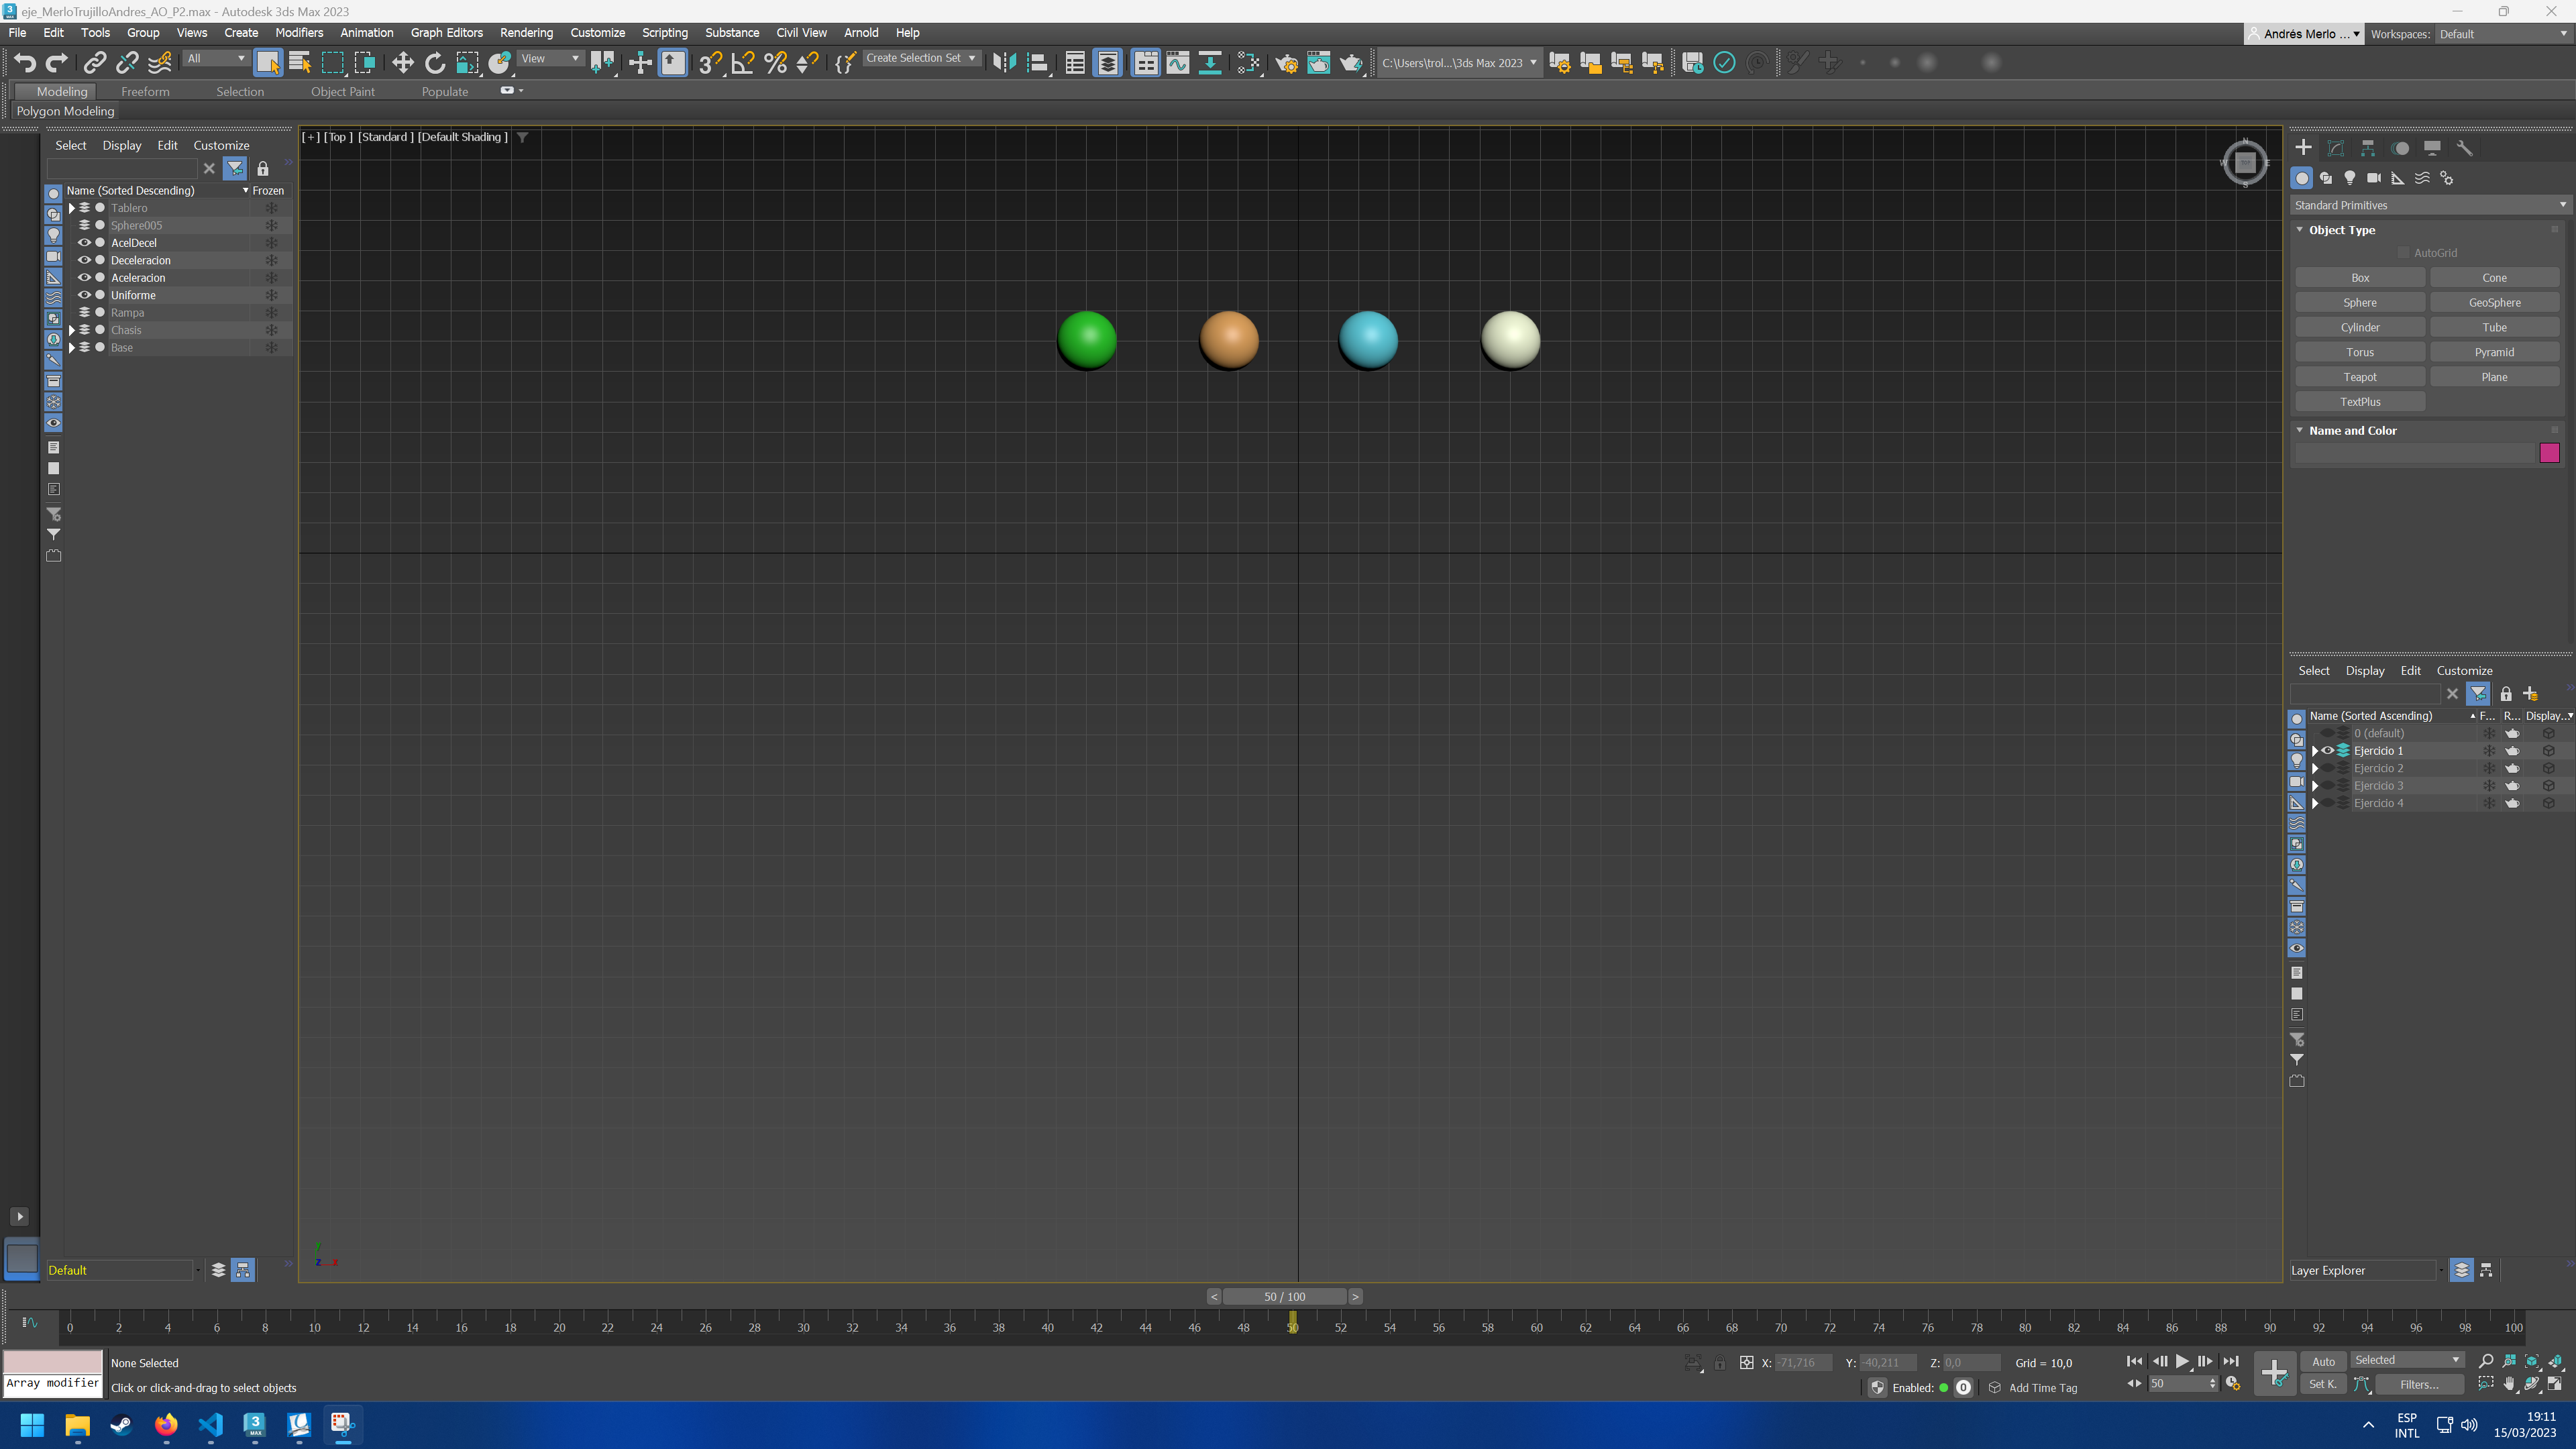
\includegraphics[width=\textwidth]{imagenes/Ejercicio 1/keyframes/50.png}
        \caption{Pelotas en el instante 50.}
    \end{subfigure}    
\end{figure}

\bigskip

Estas animaciones las voy a dividir en subsecciones para explicar mejor como son las curvas:

\subsection{Movimiento uniforme}

Para esta animación es necesario utilizar una curva lineal, que permita avanzar siempre la misma distancia en cada instante de tiempo. La función tiene la siguiente forma:

%foto de la curva
\begin{figure}[H]
   \centering
   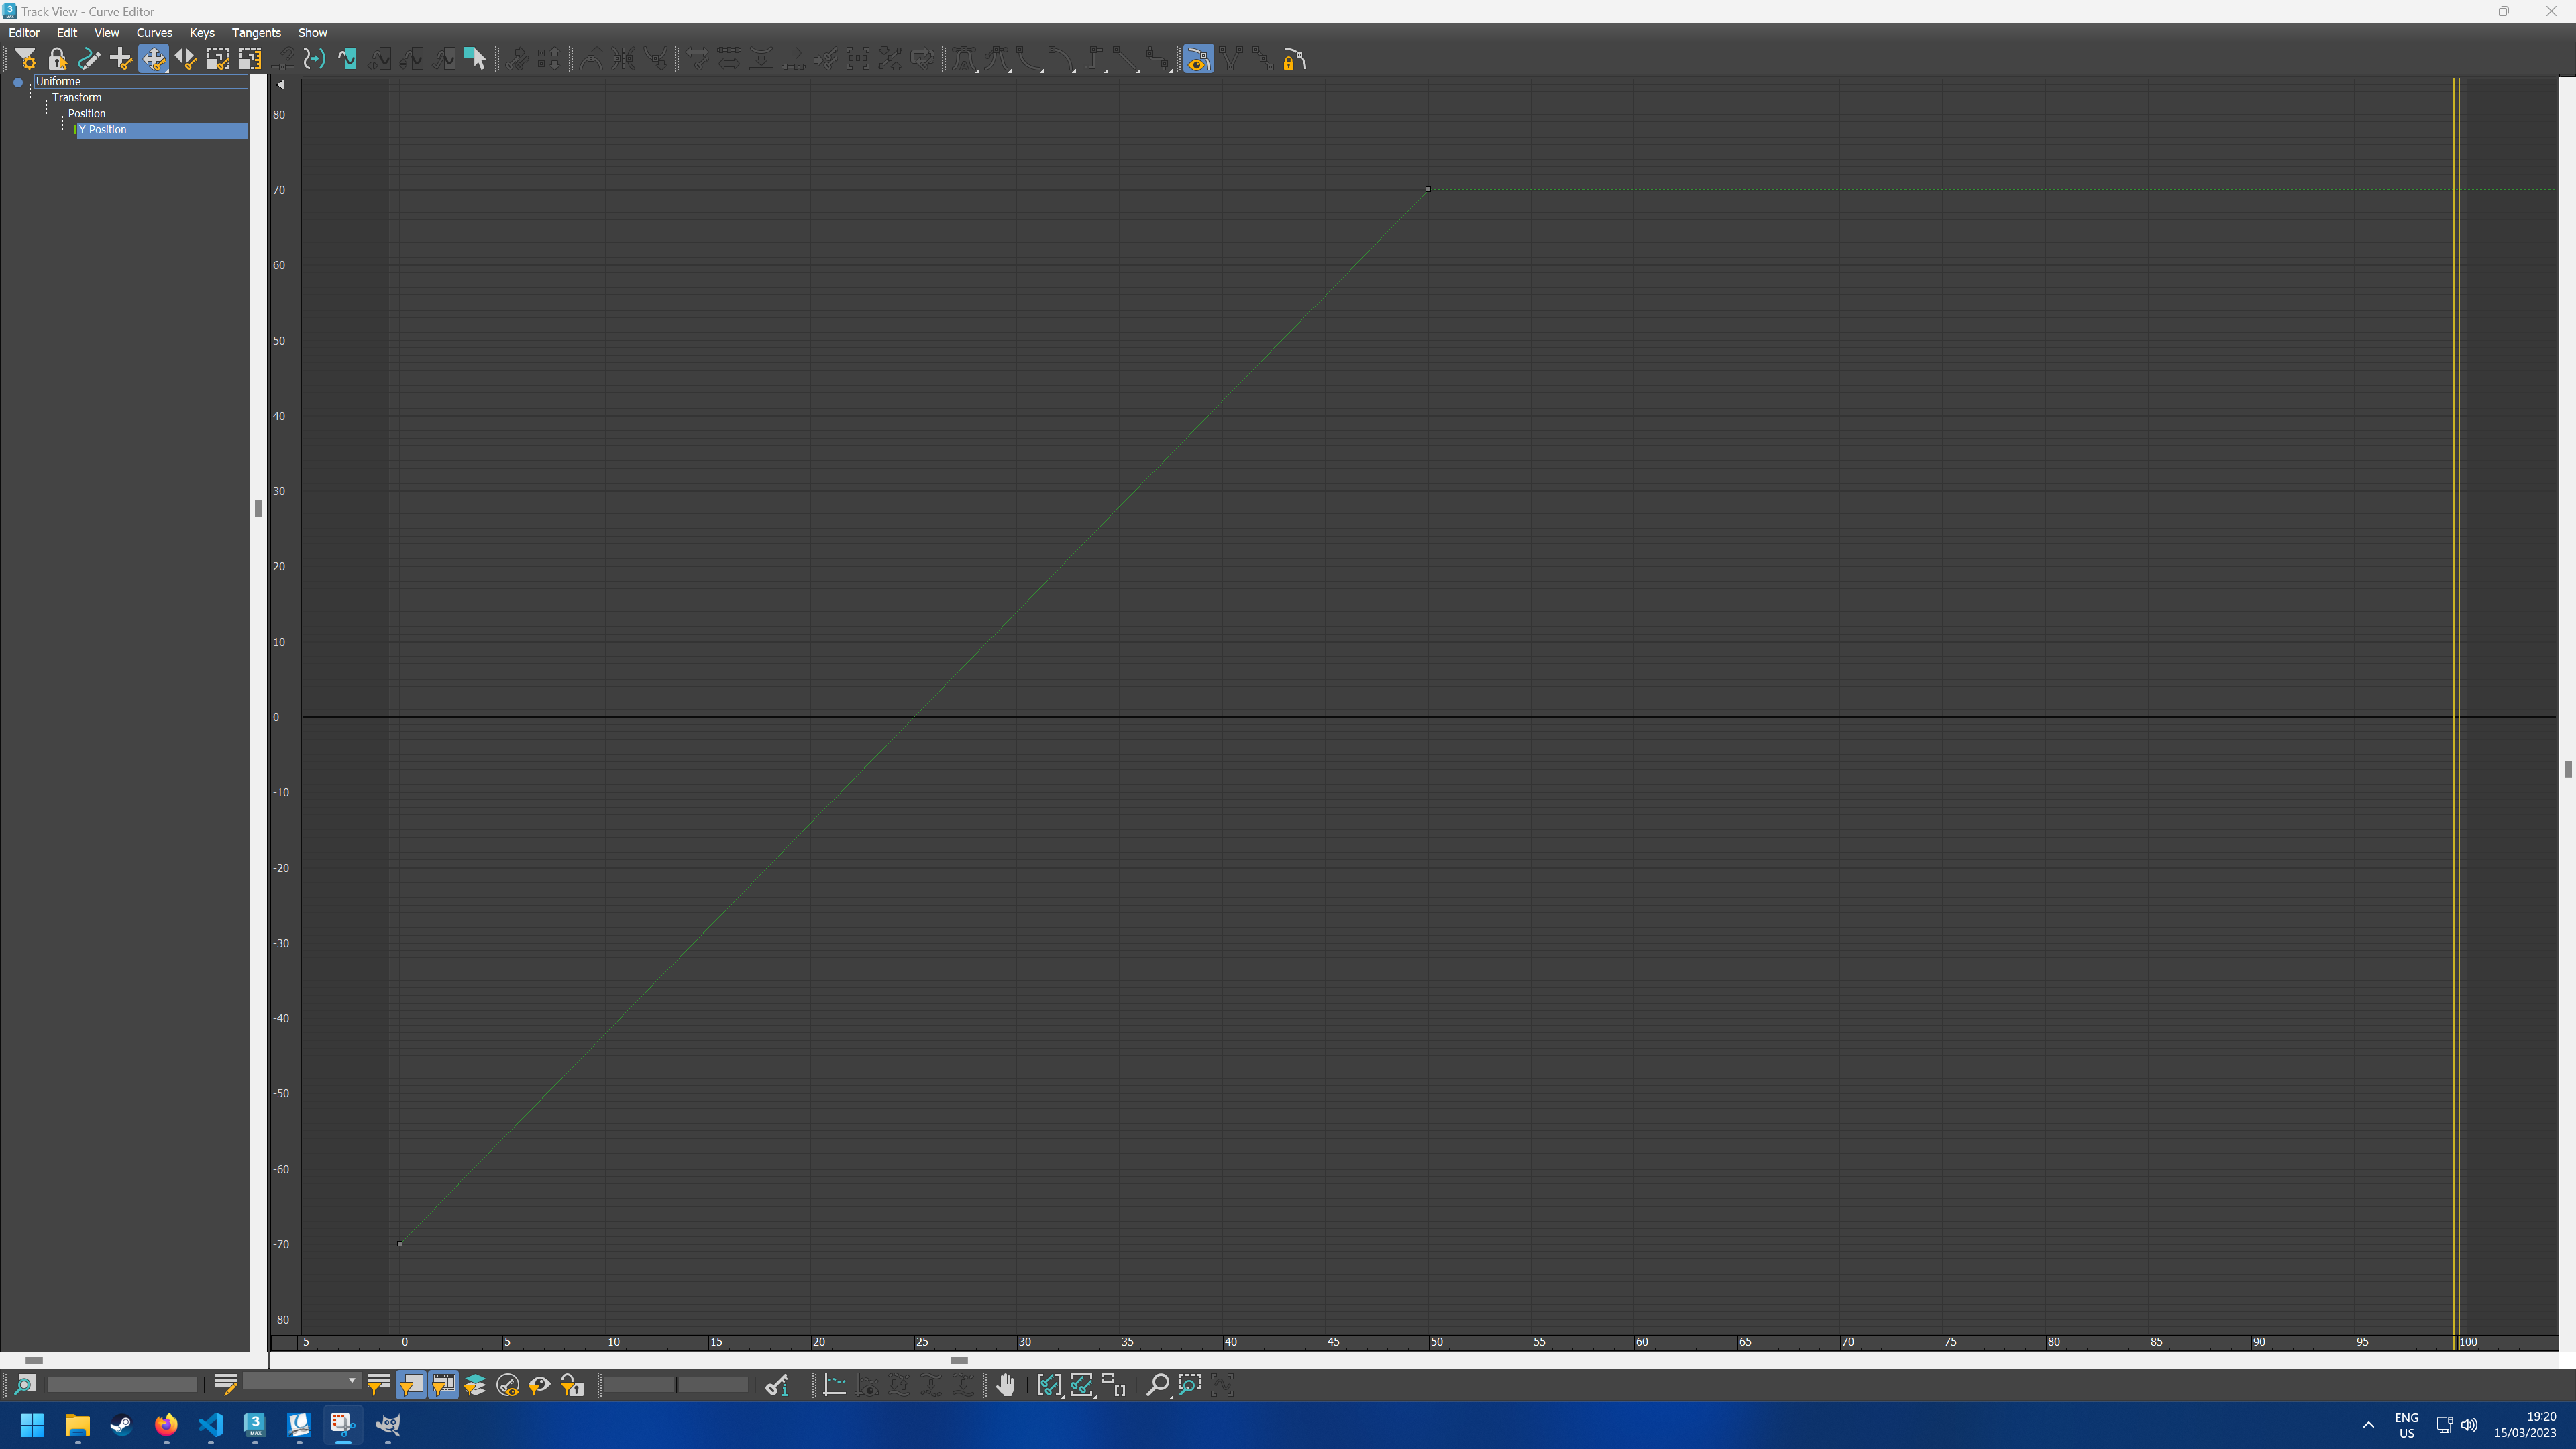
\includegraphics[width=\textwidth]{imagenes/Ejercicio 1/curvas/uniforme.png}
   \caption{Curva de la pelota con movimiento uniforme.}
\end{figure}

En la animación se puede apreciar cómo la pelota mantiene su velocidad constante desde la posición inicial hasta la final.
\subsection{Aceleración}

Para realizar esta animación se debe usar una curva de aceleración cuya pendiente sea creciente. Esto hará que la pelota recorra progresivamente una mayor distancia en la misma cantidad de tiempo.

La curva tiene la siguiente forma:

%foto de la grafica
\begin{figure}[H]
    \centering
    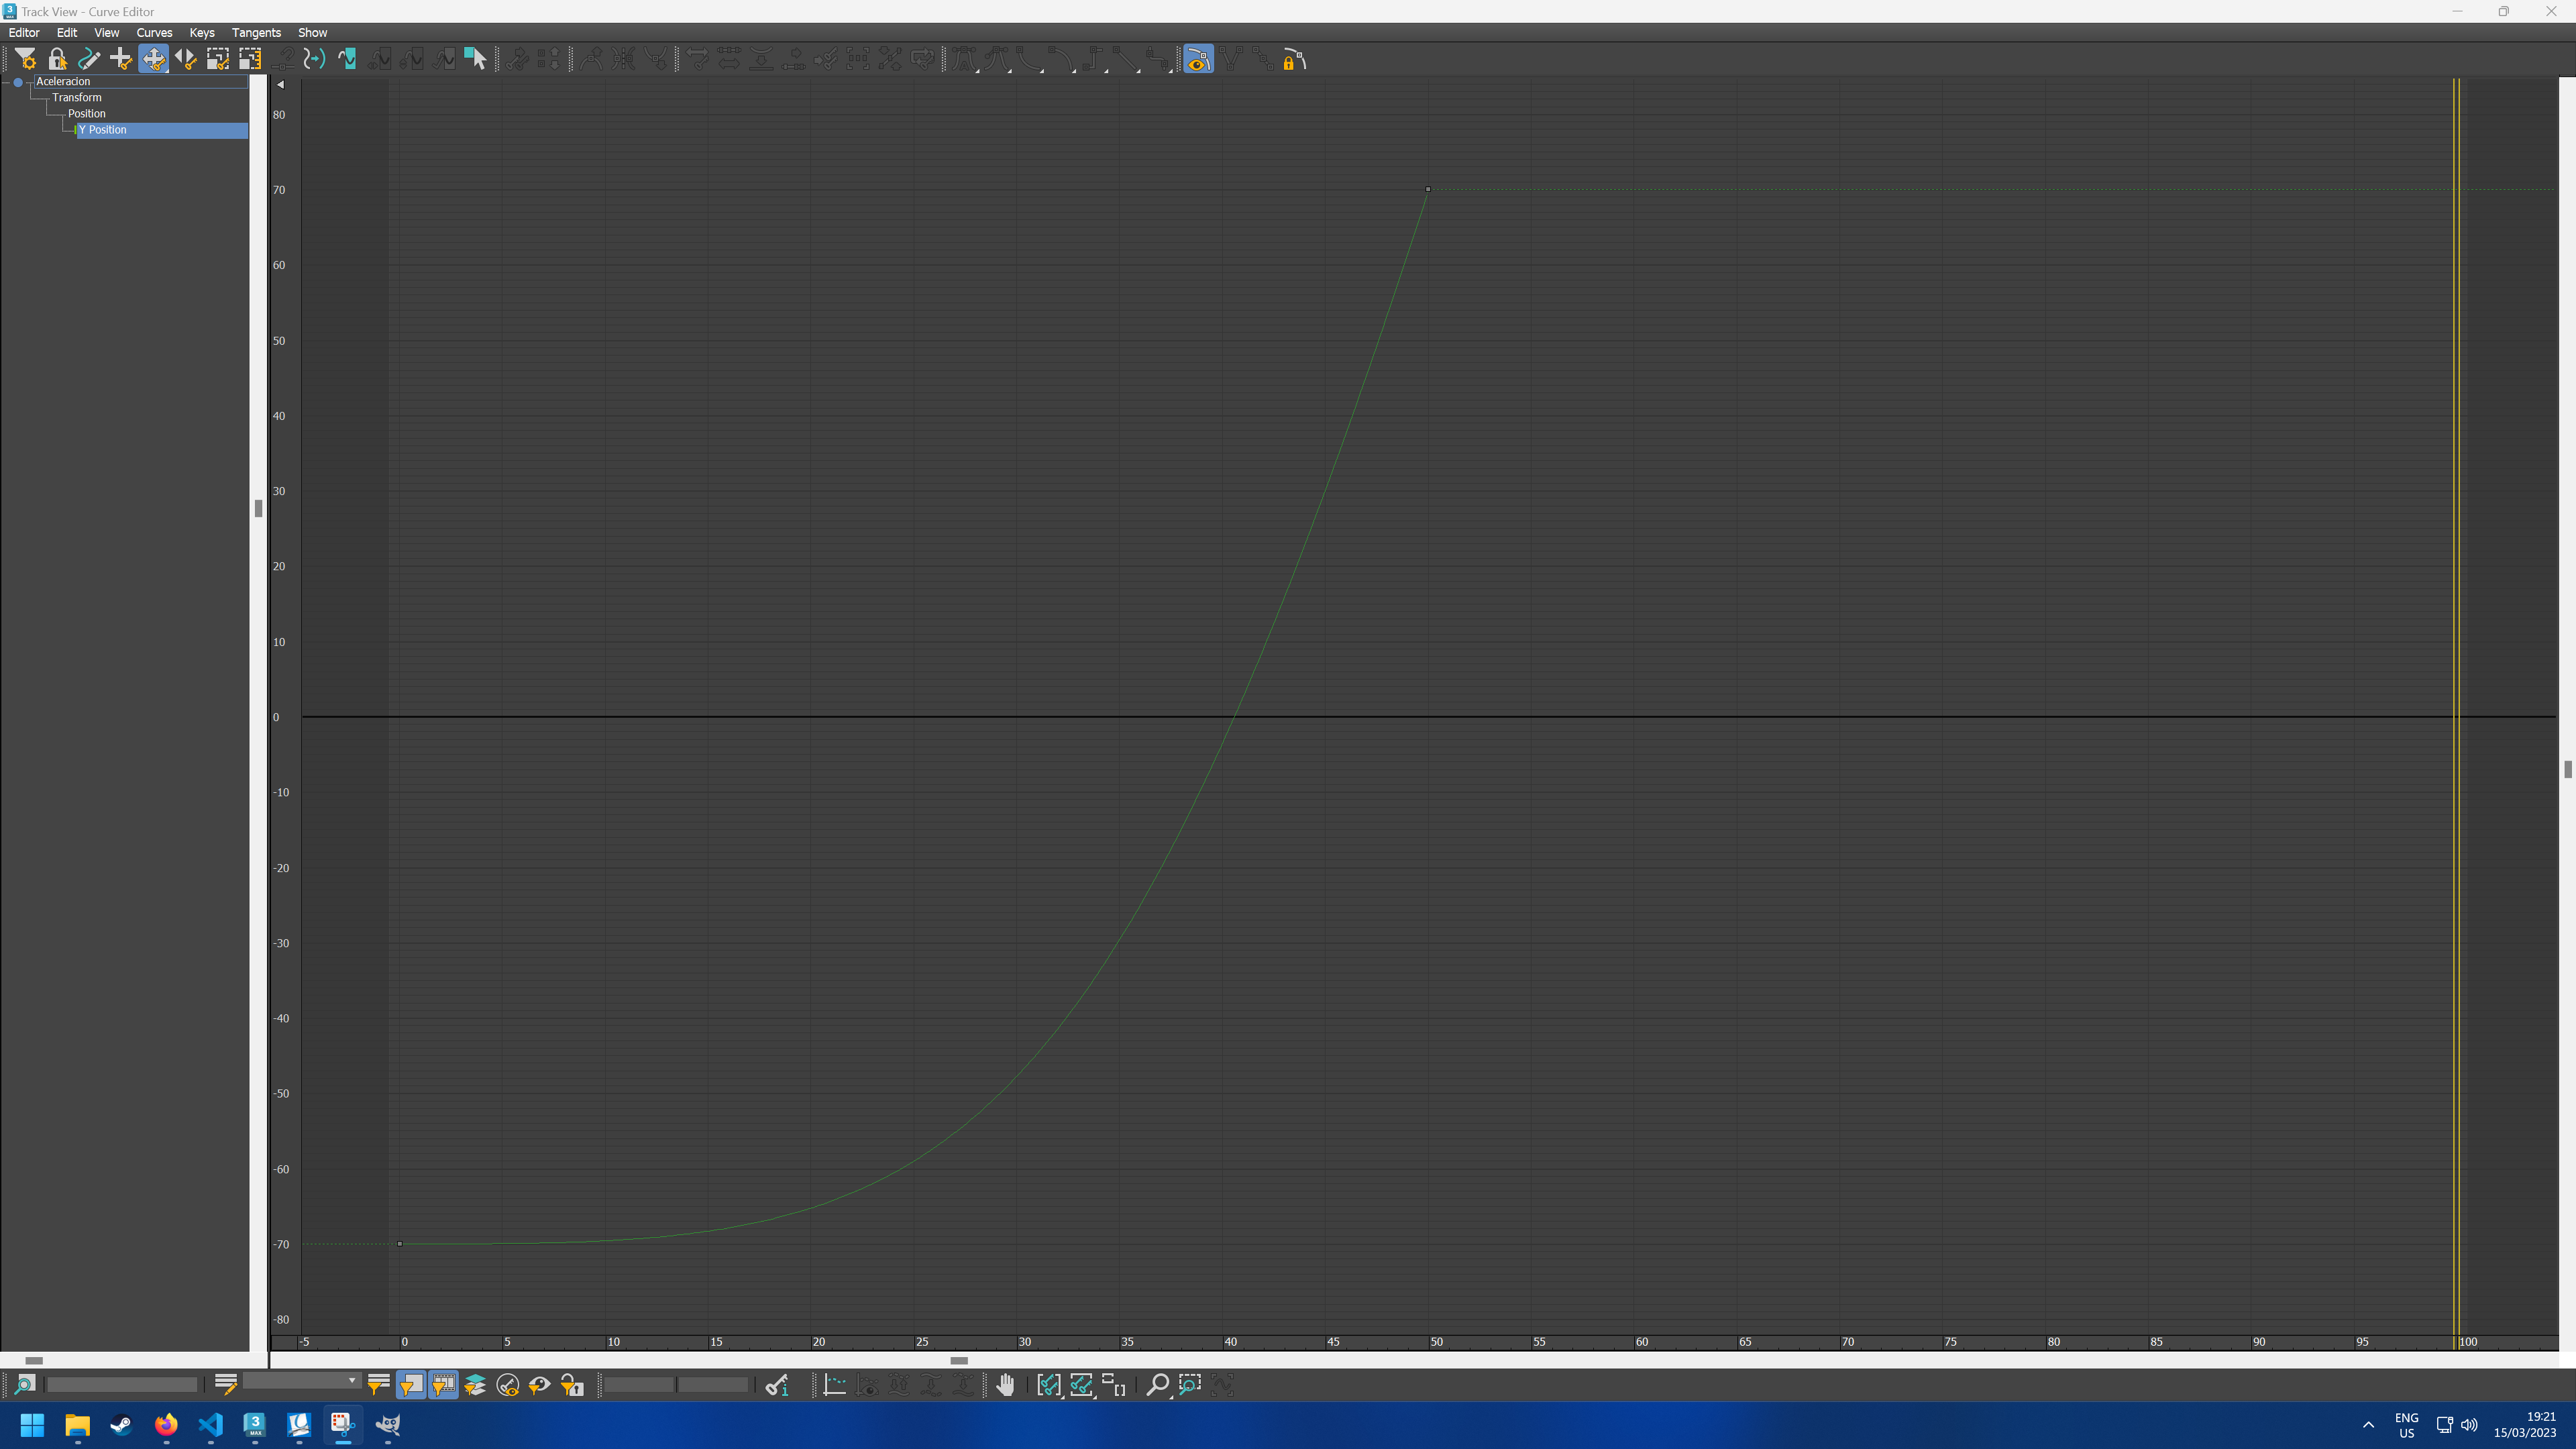
\includegraphics[width=\textwidth]{imagenes/Ejercicio 1/curvas/aceleracion.png}
    \caption{Curva de la pelota que acelera.}
\end{figure}

En la animación se puede observar como la pelota acelera gradualmente hasta que se detiene abruptamente en el punto B.


Cabe decir que he modificado la forma de la curva para que se pueda apreciar con mayor claridad la aceleración en la animación, dado que la curva por defecto del programa no es lo suficientemente pronunciada como para apreciarlo.

\subsection{Deceleración}

En este caso, se debe utilizar una curva de desaceleración, similar a la curva de aceleración, pero con una pendiente cada vez menor. Esto provocará que la pelota recorra una distancia cada vez menor en la misma cantidad de tiempo, logrando así que finalmente se detenga en el punto B.

La curva tiene la siguiente forma:

%foto de la curva
\begin{figure}[H]
    \centering
    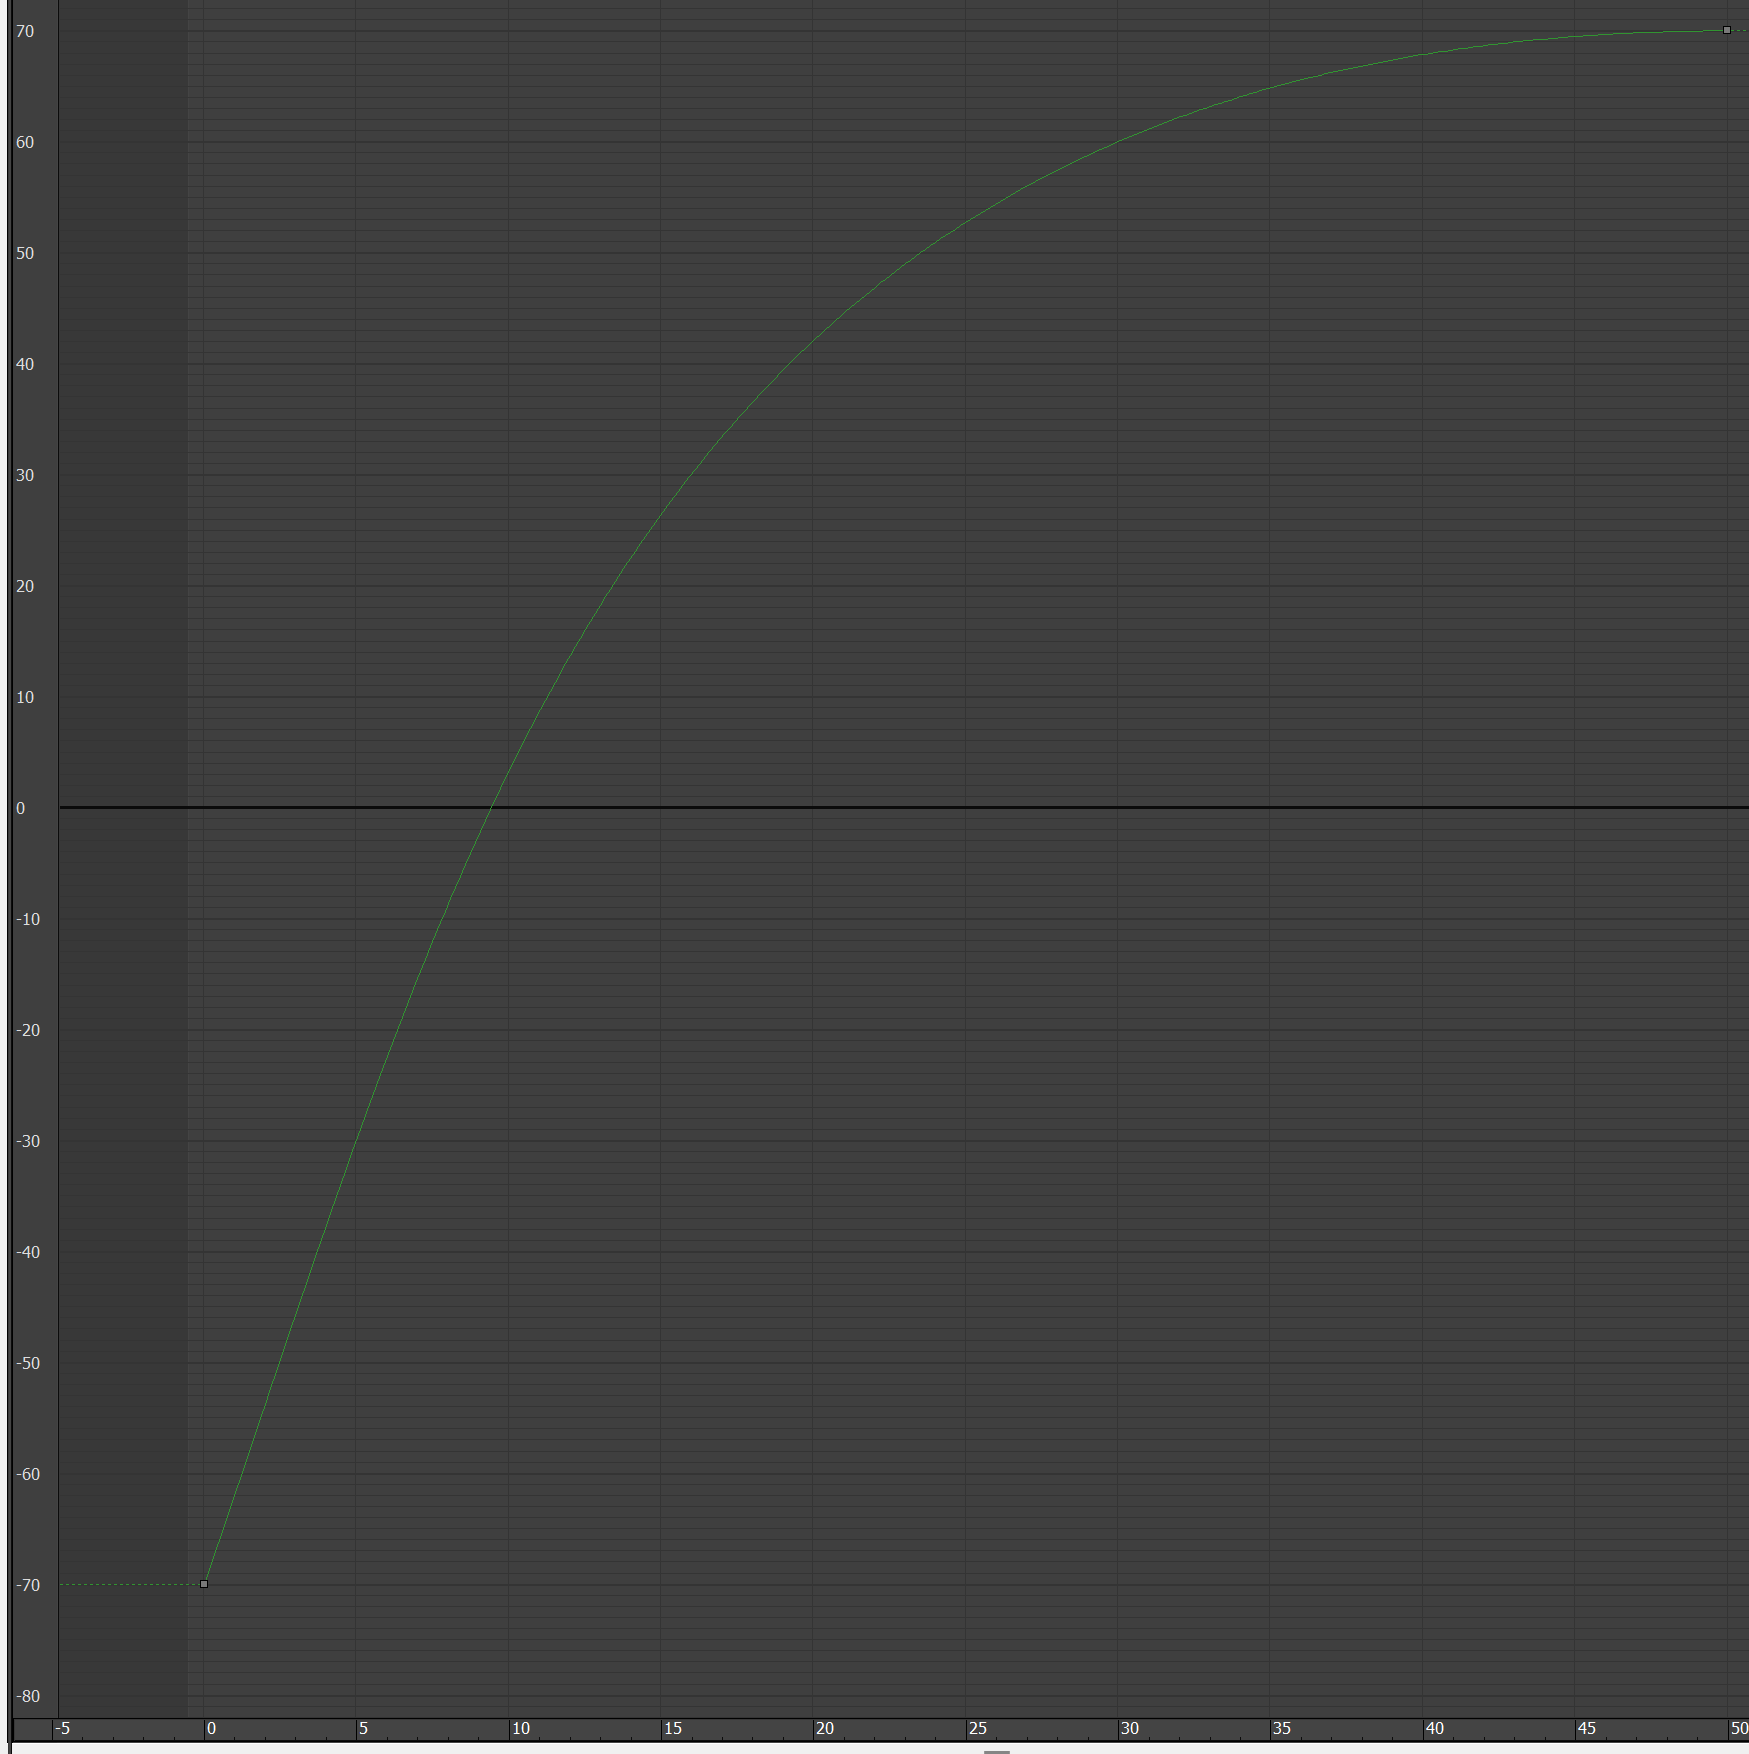
\includegraphics[width=\textwidth]{imagenes/Ejercicio 1/curvas/deceleracion.png}
    \caption{Curva de la pelota que desacelera.}
\end{figure}


En la animación, la pelota comienza moviéndose a gran velocidad y a medida que se acerca a su posición final, disminuye su velocidad hasta detenerse por completo.

Al igual que con la aceleración, he modificado la curva para que el frenado sea más pronunciado.

\subsection{Aceleración y deceleración}

% Esta animación es la combinación de la versión de aceleración y deceleración, haciendo que la pelota acelere cuando salga del punto A y vaya frenando cuando se acerque al punto B. 

Esta animación es el resultado de combinar las versiones de aceleración y deceleración, lo que provoca que la pelota acelere al salir del punto A y desacelere al acercarse al punto B.

% La curva resultante es la unión de ambas versiones, haciendo que la pendiente sea progresivamente creciente, hasta llegar a un punto en el que la pendiente decrece. 

La curva resultante es la unión de ambas versiones, con una pendiente que aumenta progresivamente hasta alcanzar un punto en el que comienza a disminuir.

Dicha curva es la siguiente:

%imagen de la curva
\begin{figure}[H]
    \centering
    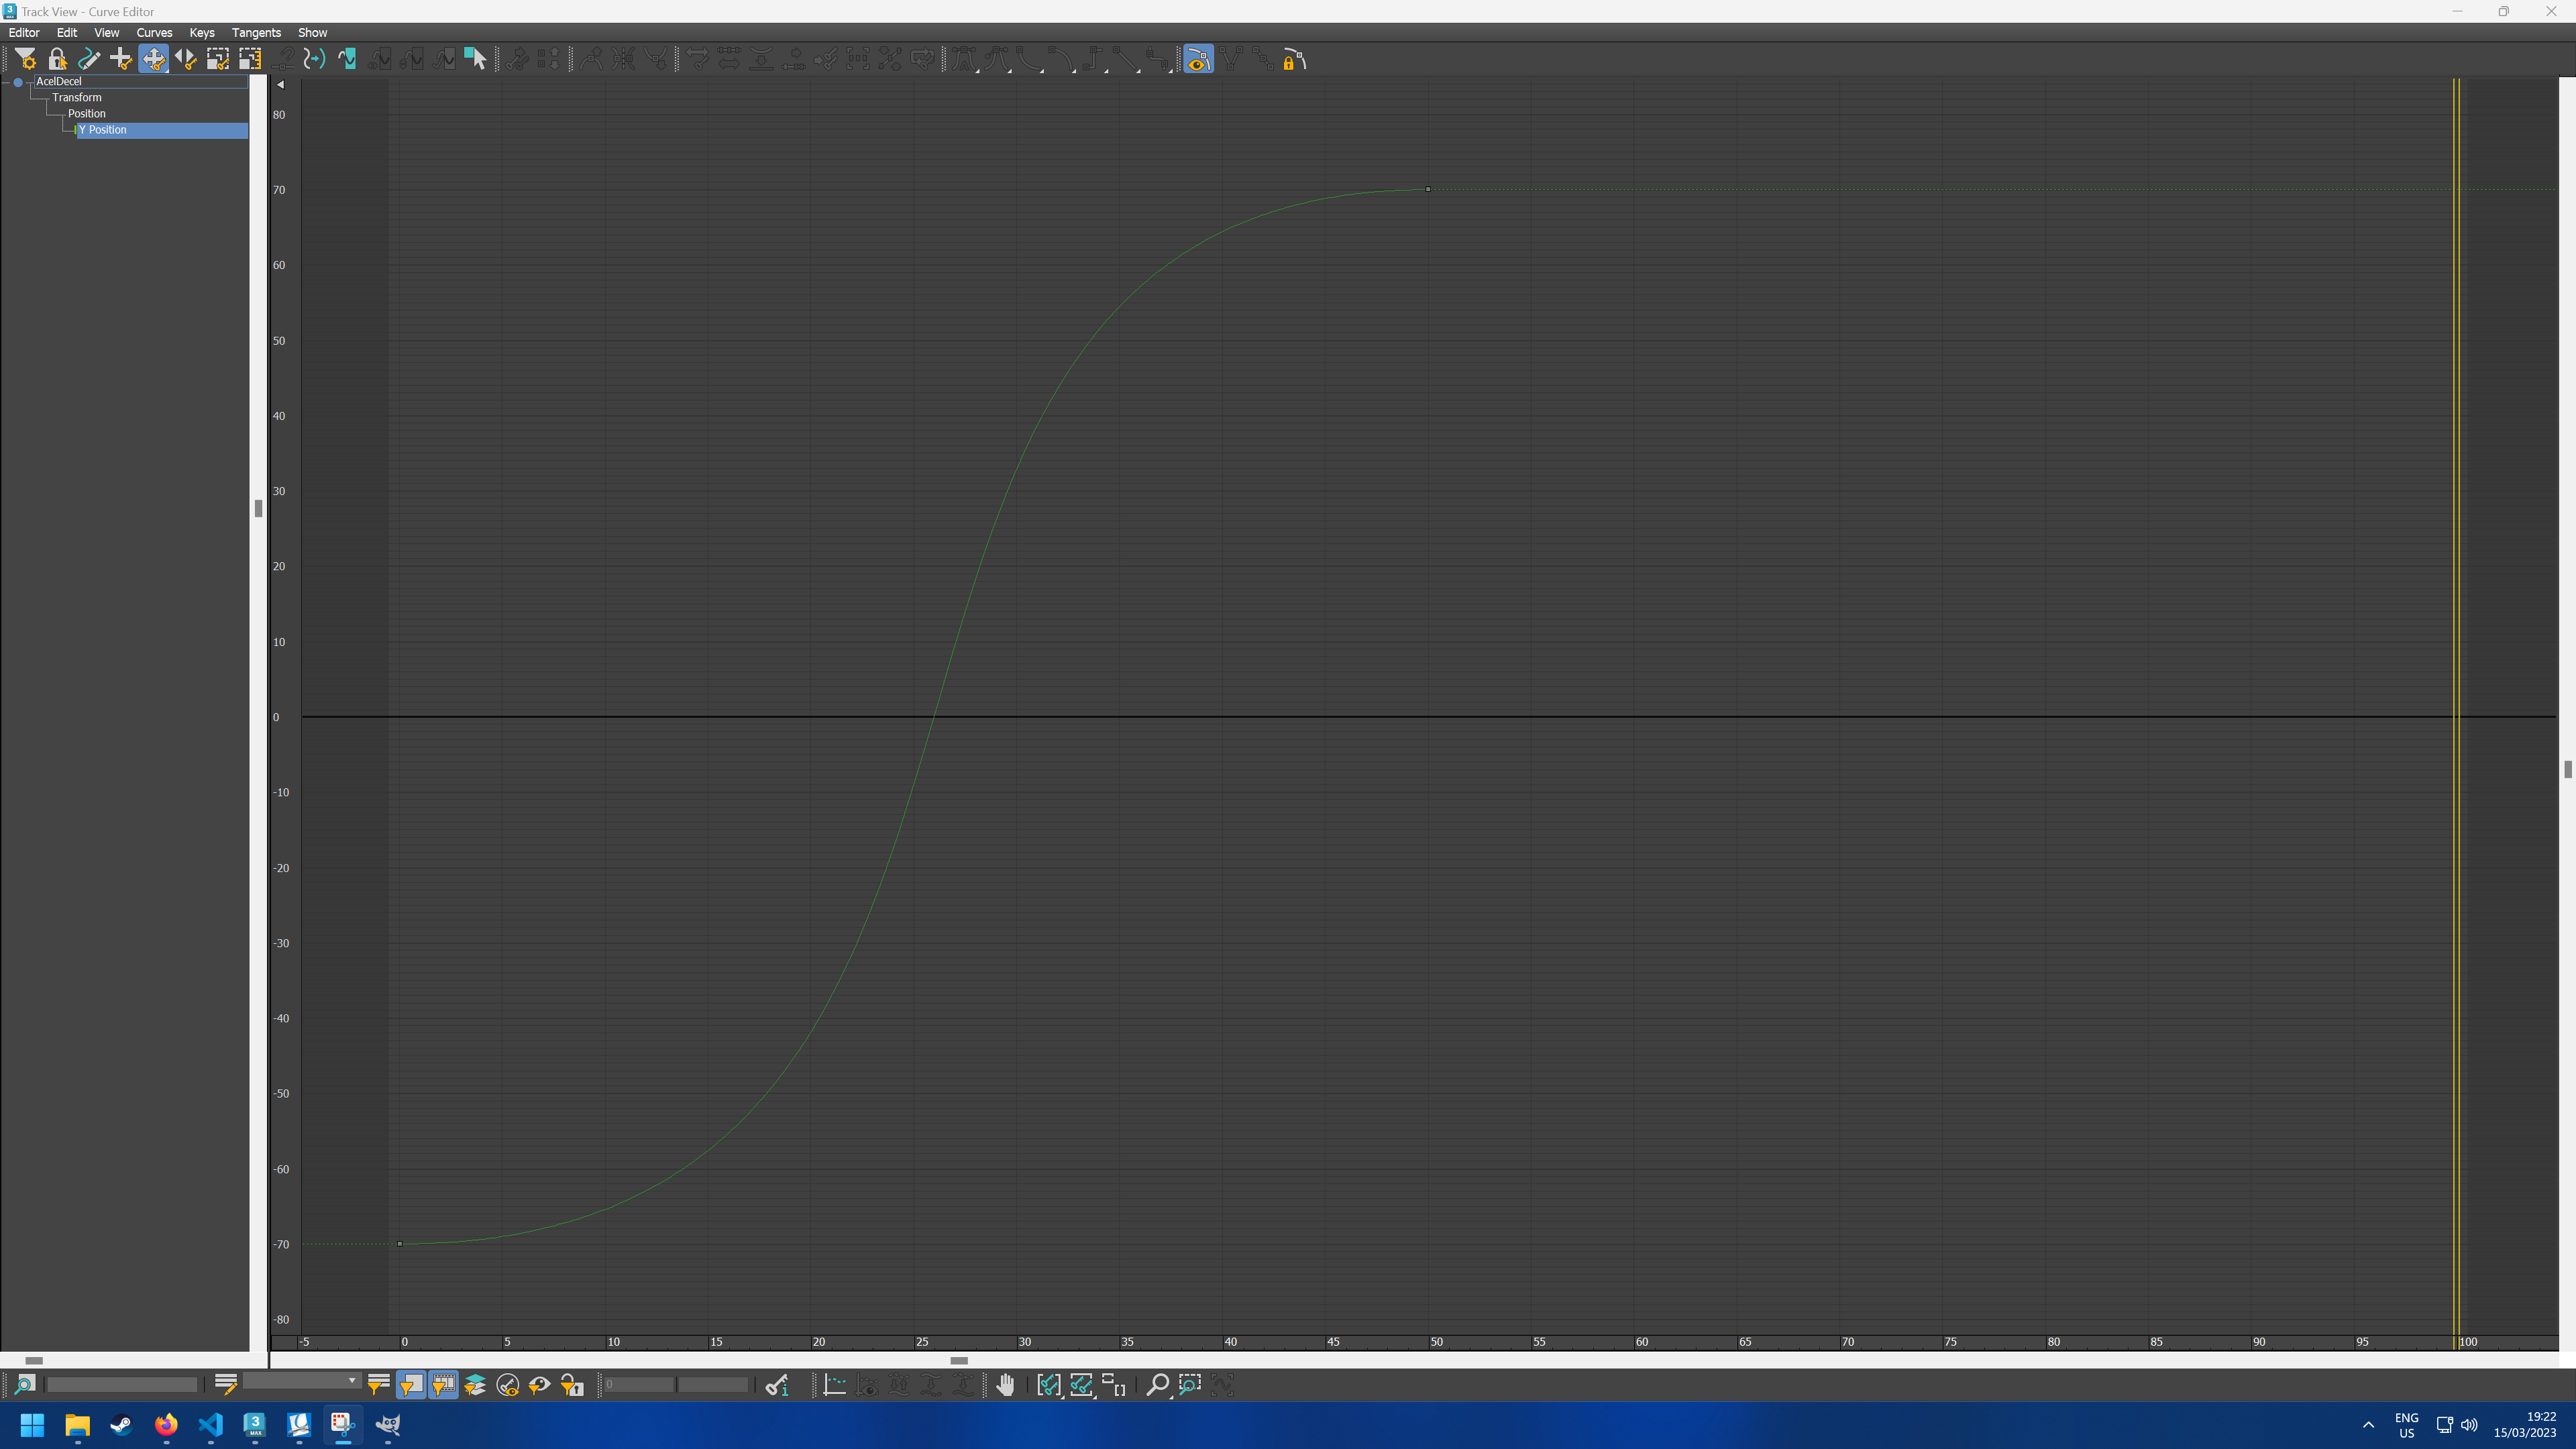
\includegraphics[width=\textwidth]{imagenes/Ejercicio 1/curvas/aceldecel.png}
    \caption{Curva de la pelota que acelera y desacelera.}
\end{figure}

% El resultado es que la pelota acelera al principio y cuando se acerca al punto final comienza a frenar. Además, como en los anteriores subsecciones, he modificado la curva para que el resultado sea más fácil de ver.

Como resultado, la pelota acelera al principio y comienza a desacelerar al acercarse al punto final. Además, al igual que en las subsecciones anteriores, he modificado la curva para que el resultado sea más fácil de apreciar.



\section{Ejercicio 2 - Salto de coche}

% En este ejercicio se pide animar un coche que arranca desde una posición, para luego subir una rampa y saltar por los aires, para finalmente cuando toca el suelo frenar.

En este ejercicio se pide animar un coche que parte desde una posición inicial, sube una rampa, la salta y finalmente frena al tocar el suelo.

% no se si poner como he hecho la rampa.

%reescribir esto
Cabe destacar que para animar la rotación necesaria para subir a la rampa, he cambiado el pivote del coche para que se sitúe justo en el eje de las ruedas traseras, ya que esto representa mejor el movimiento real al subir dicha rampa.

% Además, la jerarquía utilizada ha sido la de dejar como padre el cubo más grande del vehículo y como hijos las ruedas y el cubo más pequeño que hace de pilares y cristales.
Además, para la jerarquía de objetos, he utilizado el cubo más grande del vehículo como padre y las ruedas y el cubo más pequeño como hijos.
}


La animación consiste en 8 \textit{keyframes}, que son los siguientes:

\begin{enumerate}
    \item Instante 0: El vehículo se encuentra en la posición inicial.
    \item Instante 13: El vehículo ha realizado la aceleración.
    \item Instante 26: El vehículo se encuentra en el instante anterior de subir la rampa.
    \item Instante 28: El vehículo ha subido la rampa y se encuentra al principio de la misma.
    \item Instante 32: El vehículo se encuentra en el instante anterior de estar en el aire; es decir, se encuentra tocando el final de la rampa solo con la rueda trasera.
    \item Instante 44: El vehículo se encuentra en el punto más alto del lanzamiento y ya recto.
    \item Instante 56: El vehículo ha tocado el suelo después del salto.
    \item Instante 85: Finalmente, el vehículo frena hasta pararse del todo.
\end{enumerate}

A modo visual, los \textit{keyframes} son los siguientes:

%fotos de los keyframes
\begin{figure}[H]
    \centering
    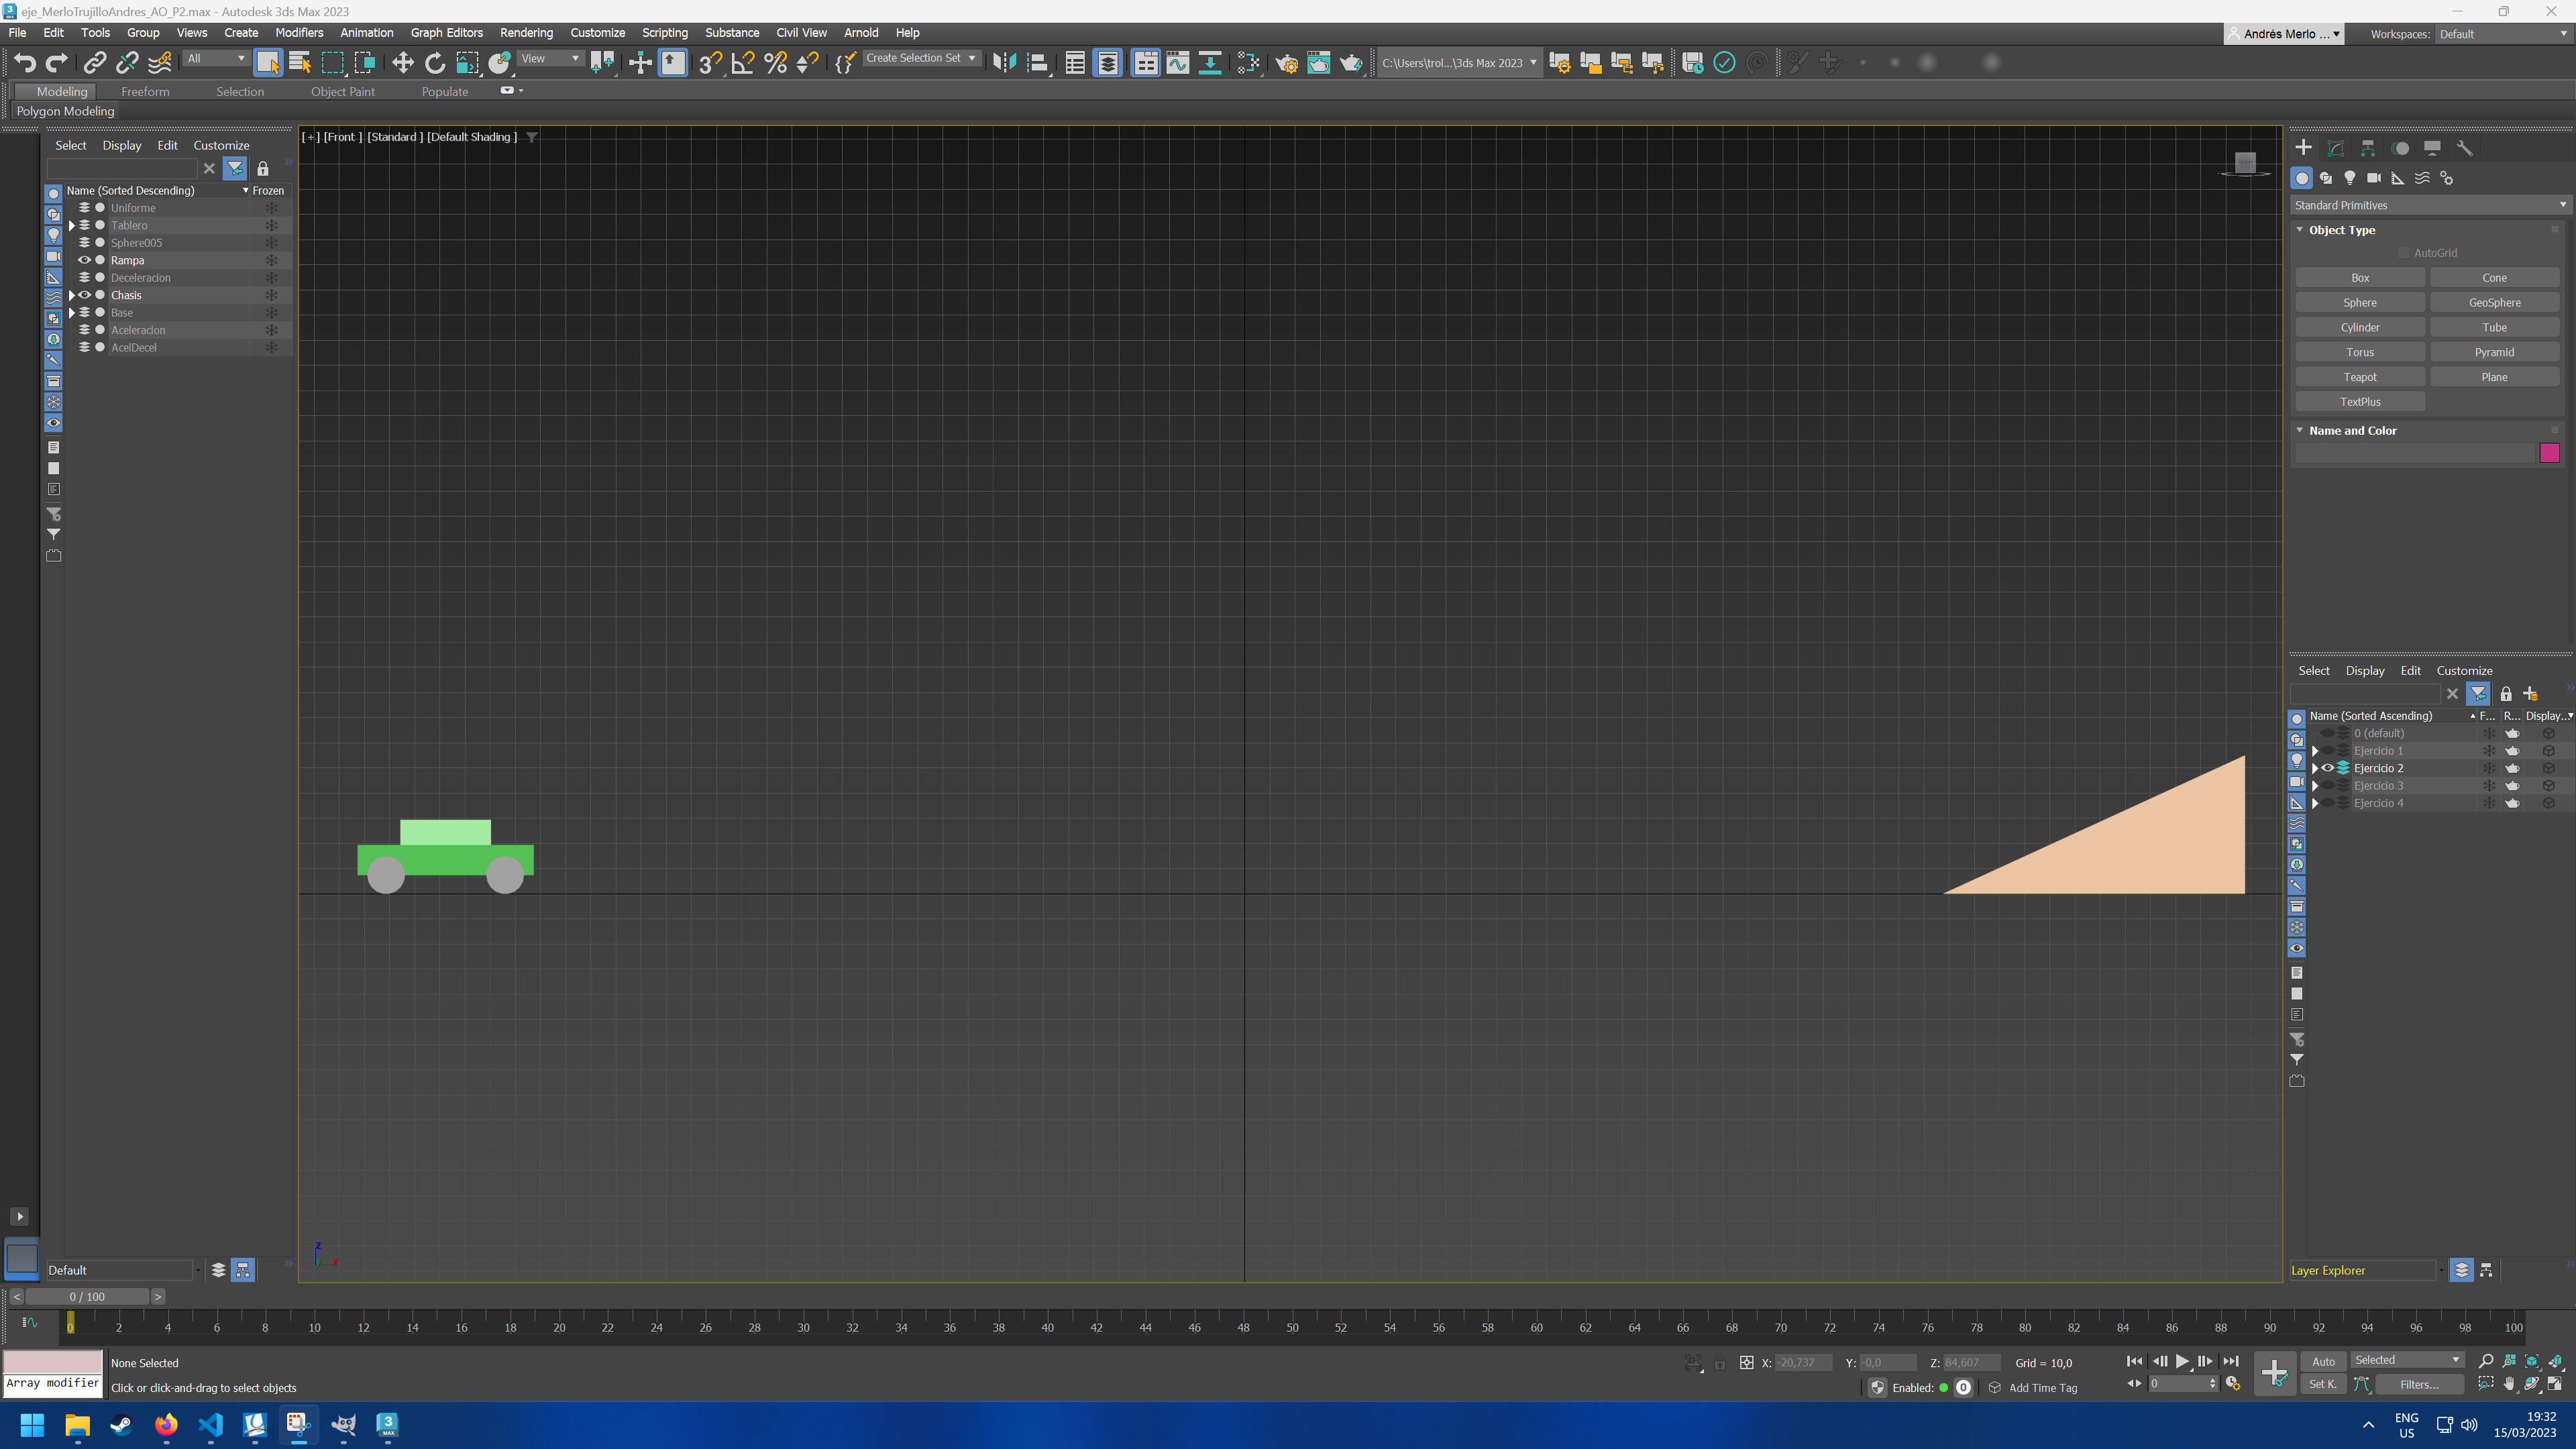
\includegraphics[width=\textwidth]{imagenes/Ejercicio2/keyframes/0.png}
    \caption{Vehículo en el instante 0.}
 \end{figure}
 \begin{figure}[H]
    \centering
    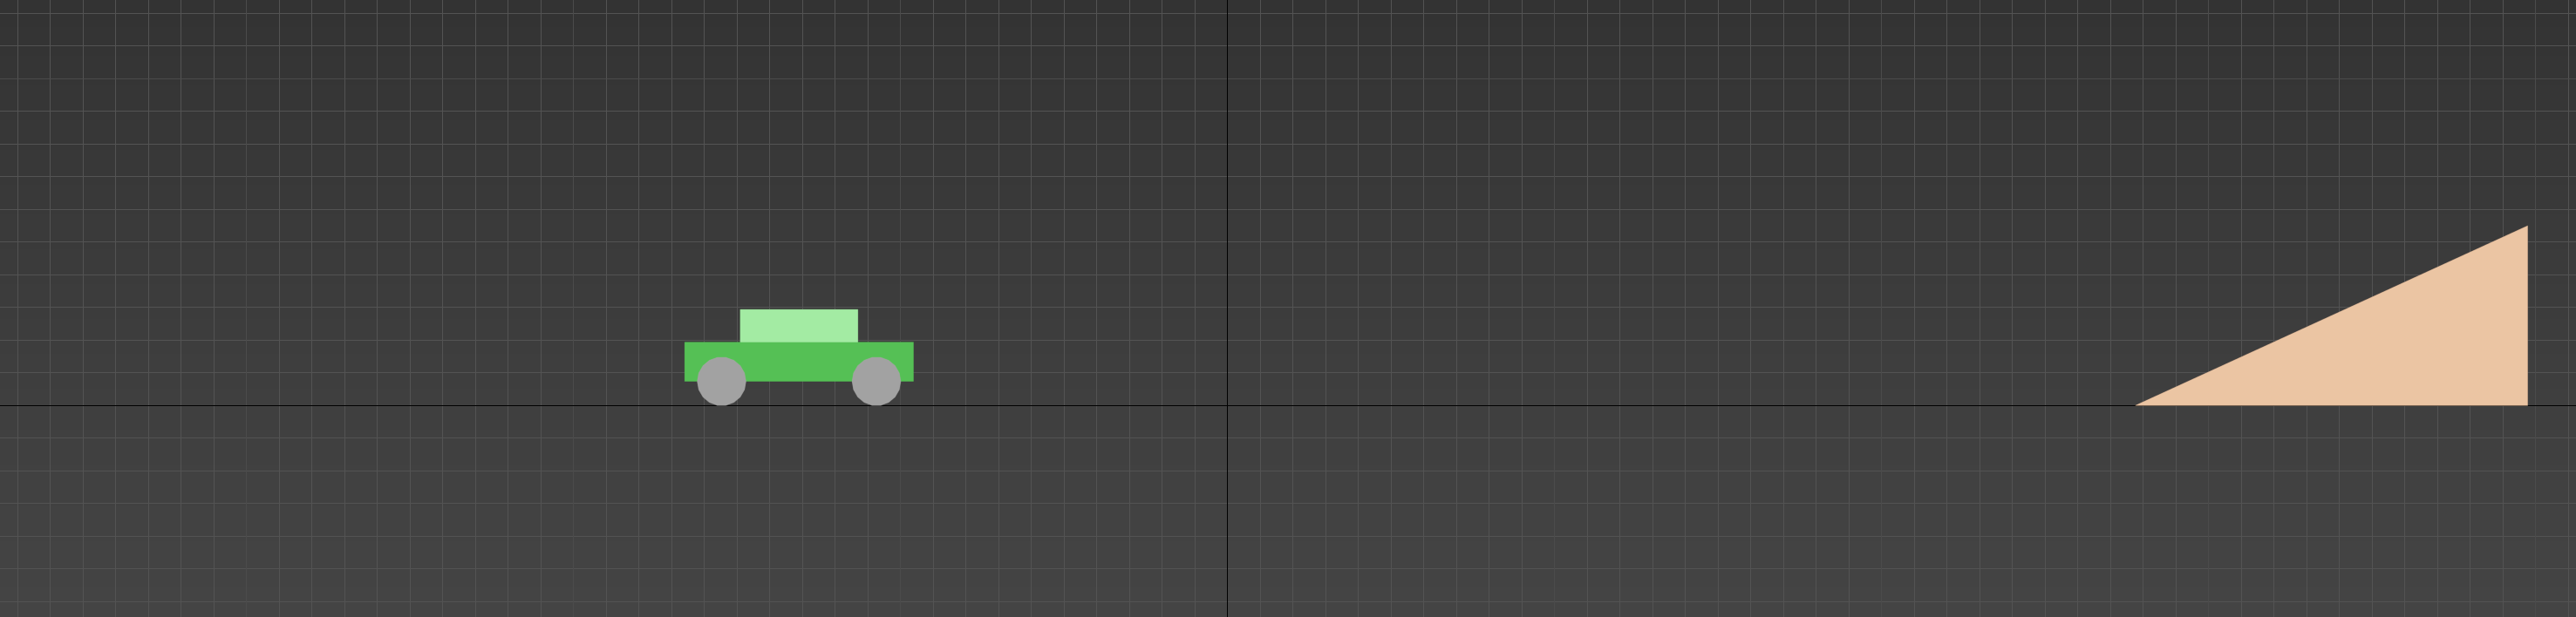
\includegraphics[width=\textwidth]{imagenes/Ejercicio2/keyframes/13.png}
    \caption{Vehículo en el instante 13.}
 \end{figure}
 \begin{figure}[H]
    \centering
    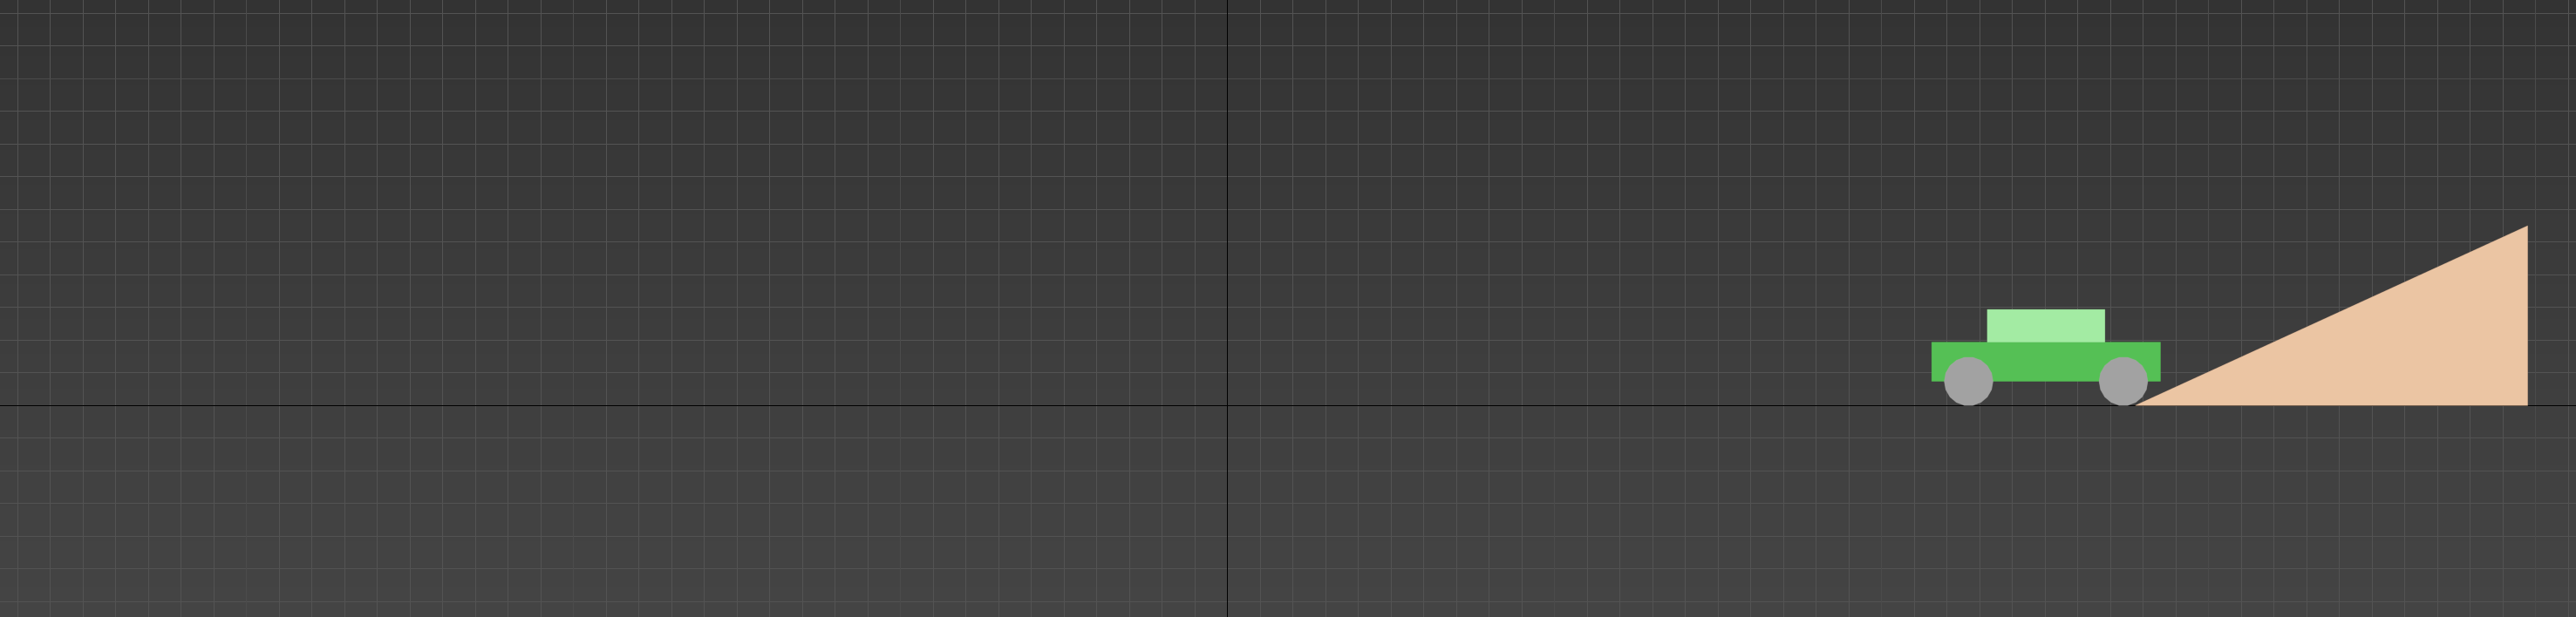
\includegraphics[width=\textwidth]{imagenes/Ejercicio2/keyframes/26.png}
    \caption{Vehículo en el instante 26.}
 \end{figure}
 \begin{figure}[H]
    \centering
    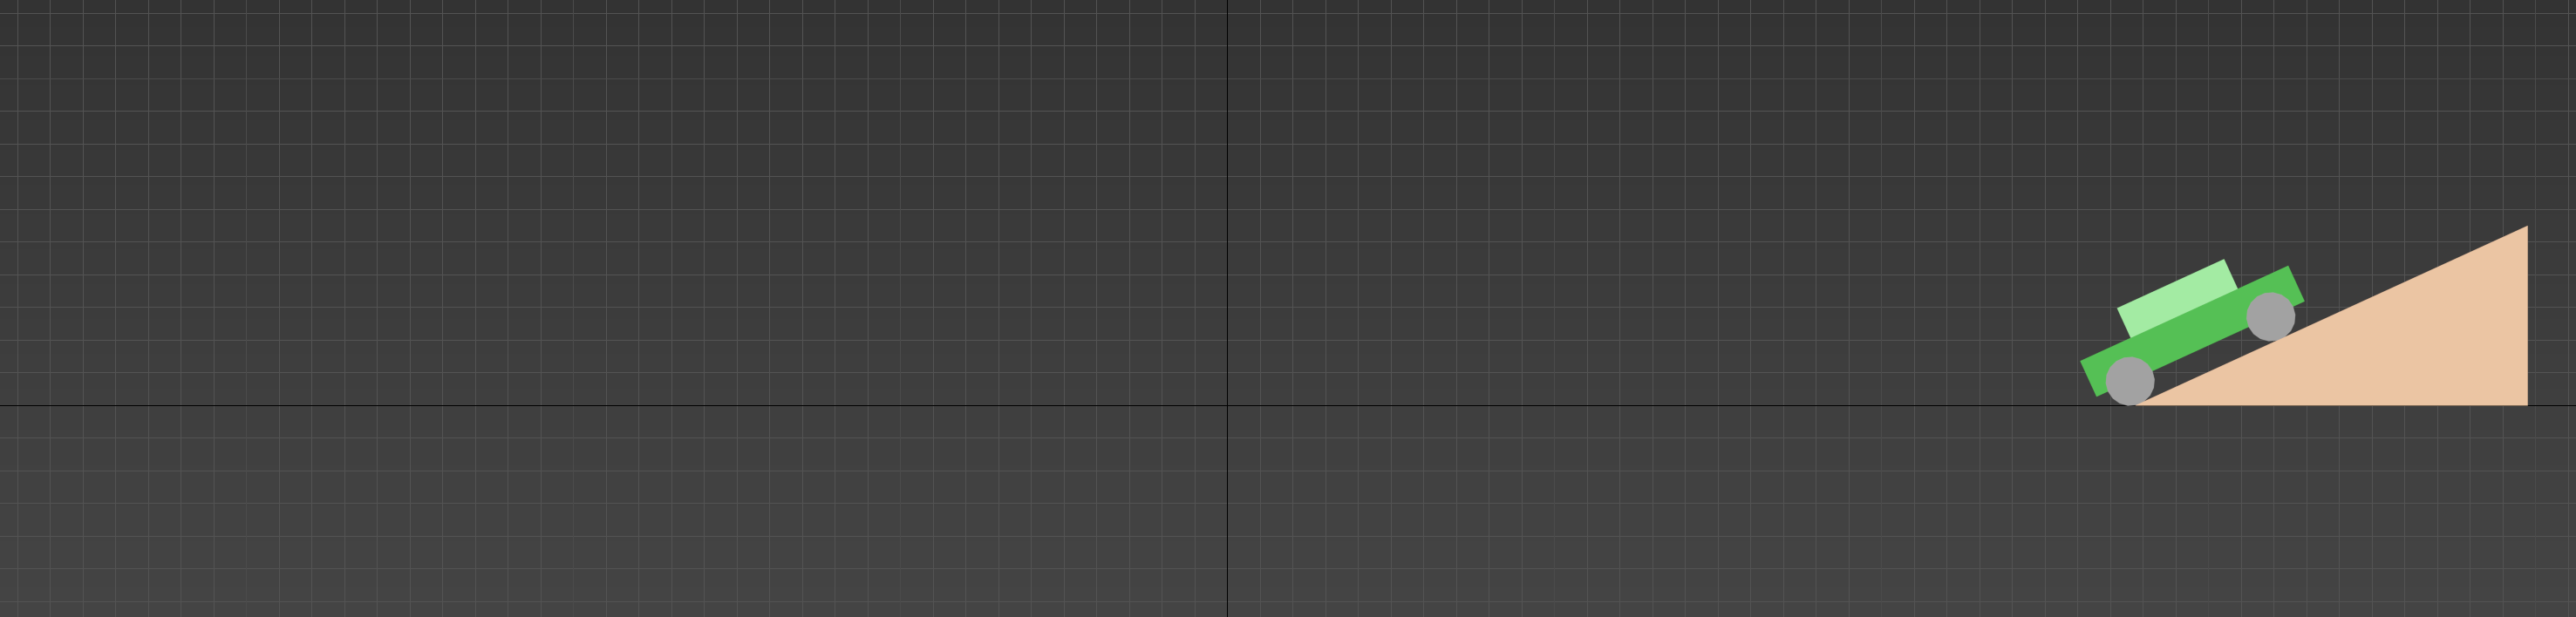
\includegraphics[width=\textwidth]{imagenes/Ejercicio2/keyframes/28.png}
    \caption{Vehículo en el instante 28.}
 \end{figure}
 \begin{figure}[H]
    \centering
    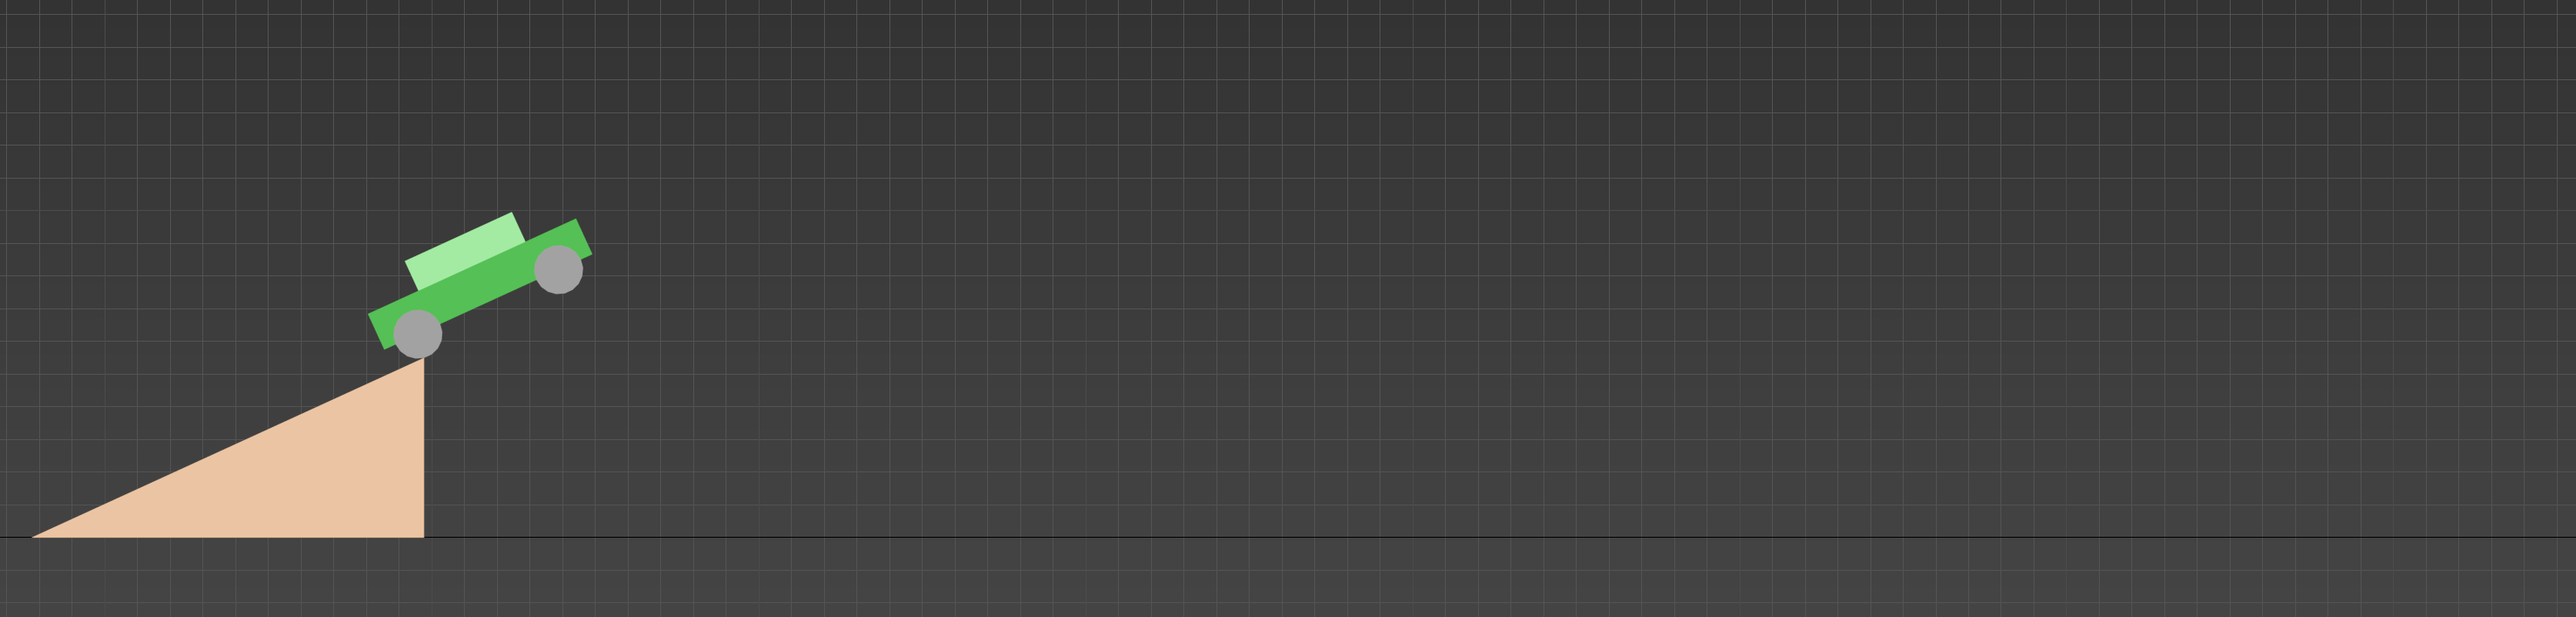
\includegraphics[width=\textwidth]{imagenes/Ejercicio2/keyframes/32.png}
    \caption{Vehículo en el instante 32.}
 \end{figure}
 \begin{figure}[H]
    \centering
    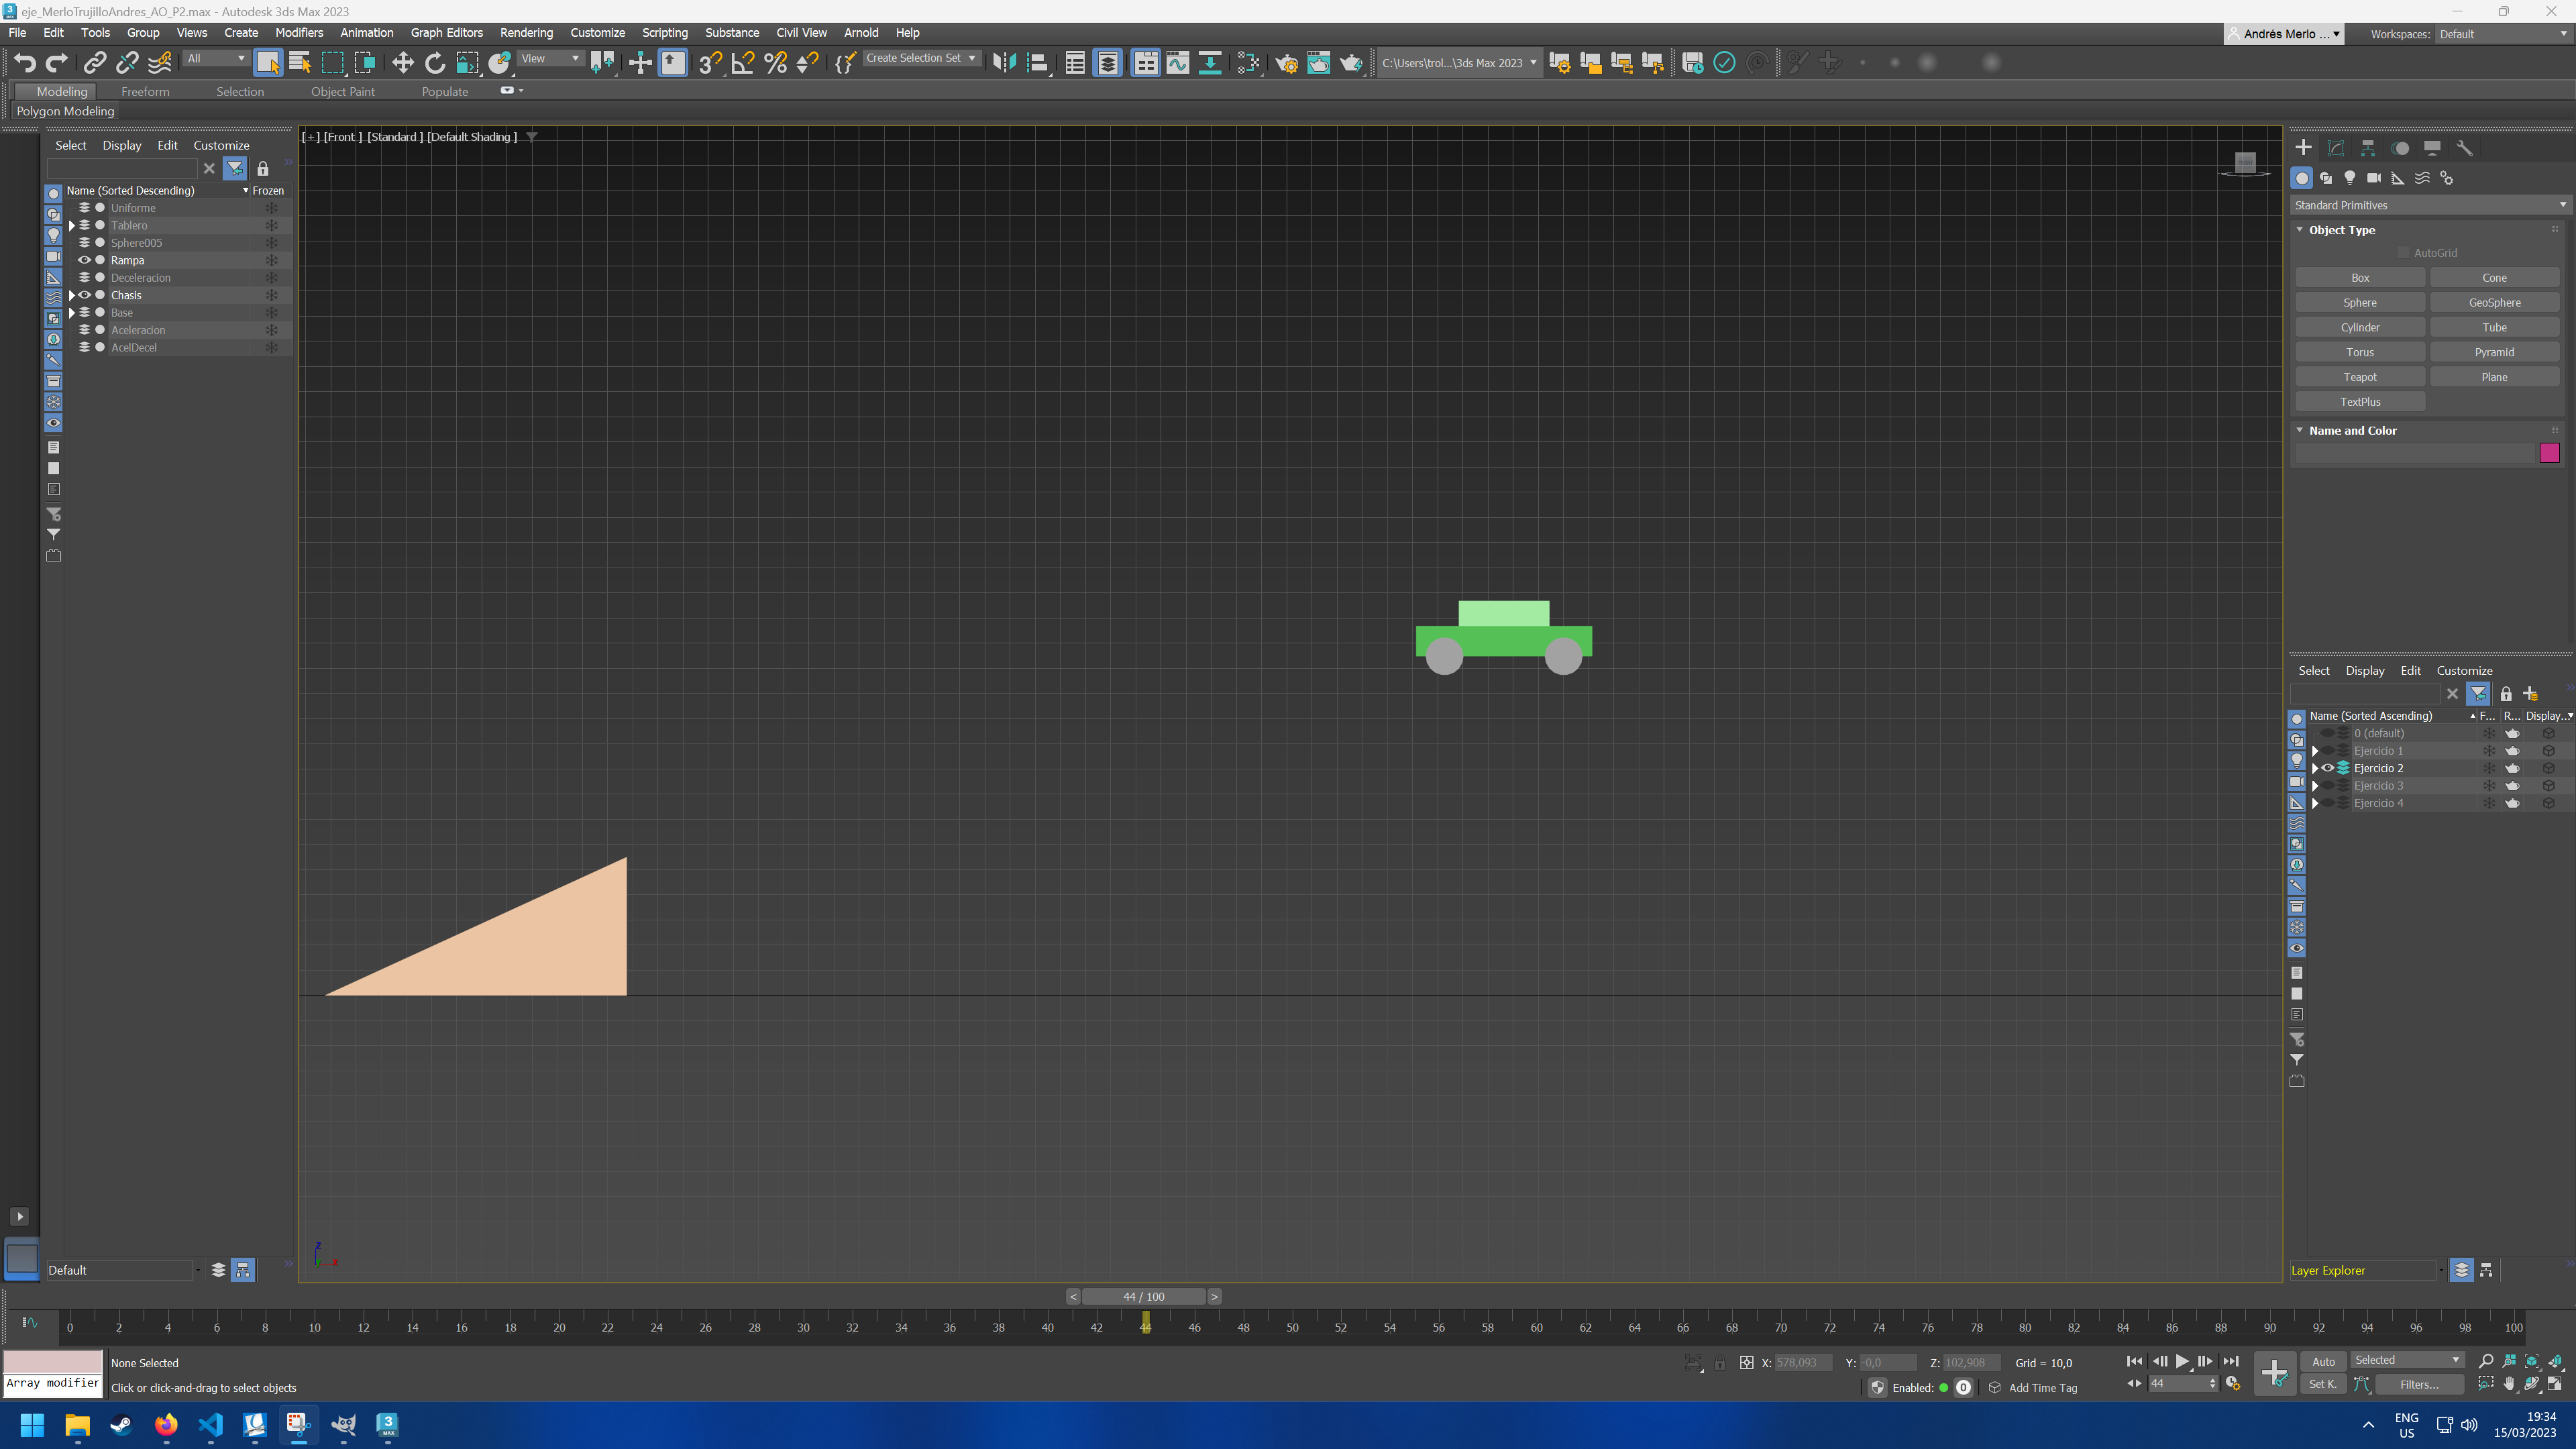
\includegraphics[width=\textwidth]{imagenes/Ejercicio2/keyframes/44.png}
    \caption{Vehículo en el instante 44.}
 \end{figure}
 \begin{figure}[H]
    \centering
    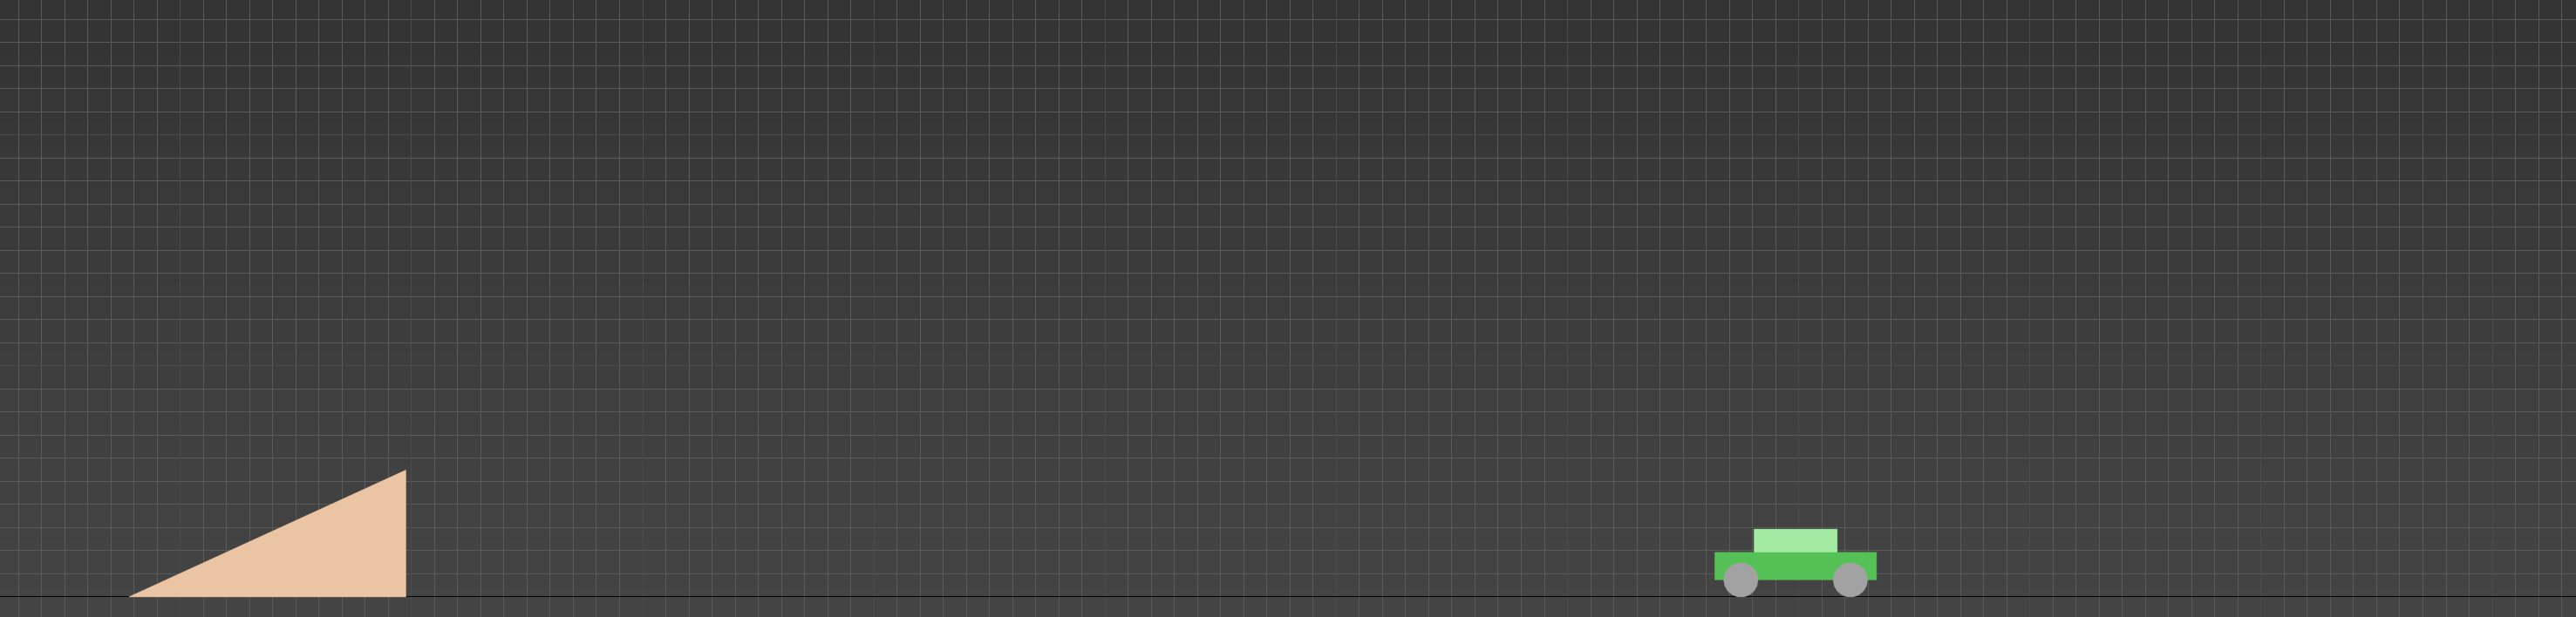
\includegraphics[width=\textwidth]{imagenes/Ejercicio2/keyframes/56.png}
    \caption{Vehículo en el instante 56.}
 \end{figure}
 \begin{figure}[H]
    \centering
    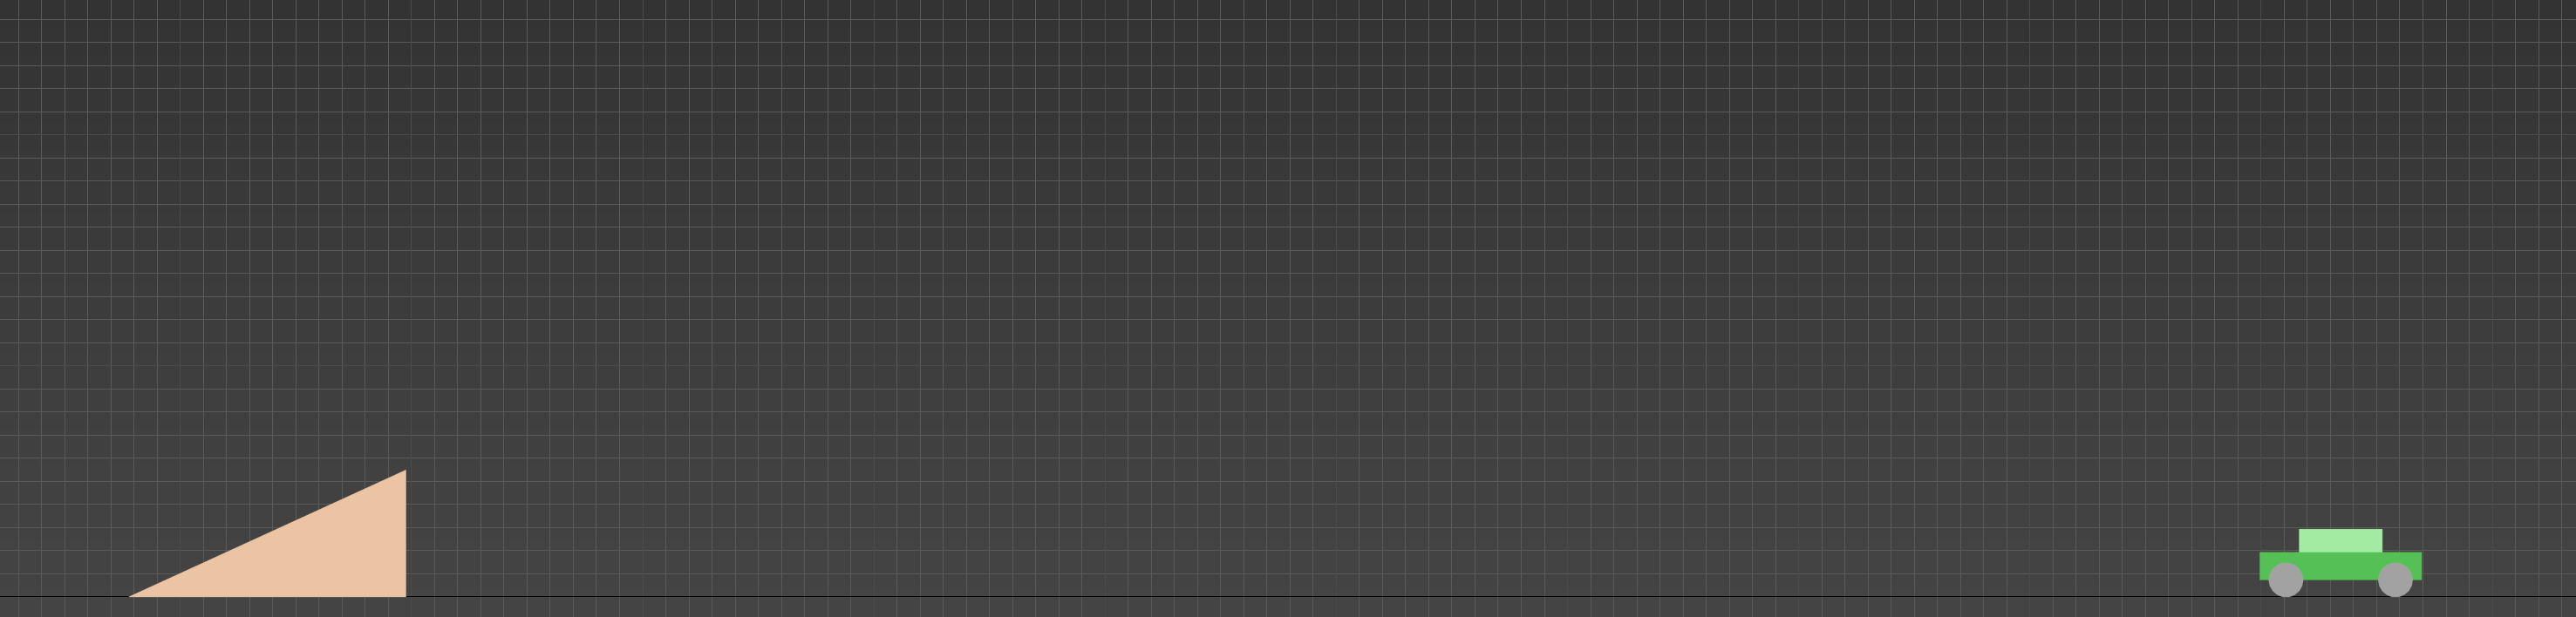
\includegraphics[width=\textwidth]{imagenes/Ejercicio2/keyframes/86.png}
    \caption{Vehículo en el instante 86.}
 \end{figure}


Y las curvas utilizadas para la animación:

%fotos de las curvas, separadas por partes (si no son muchas)
\begin{figure}[H]
    \centering
    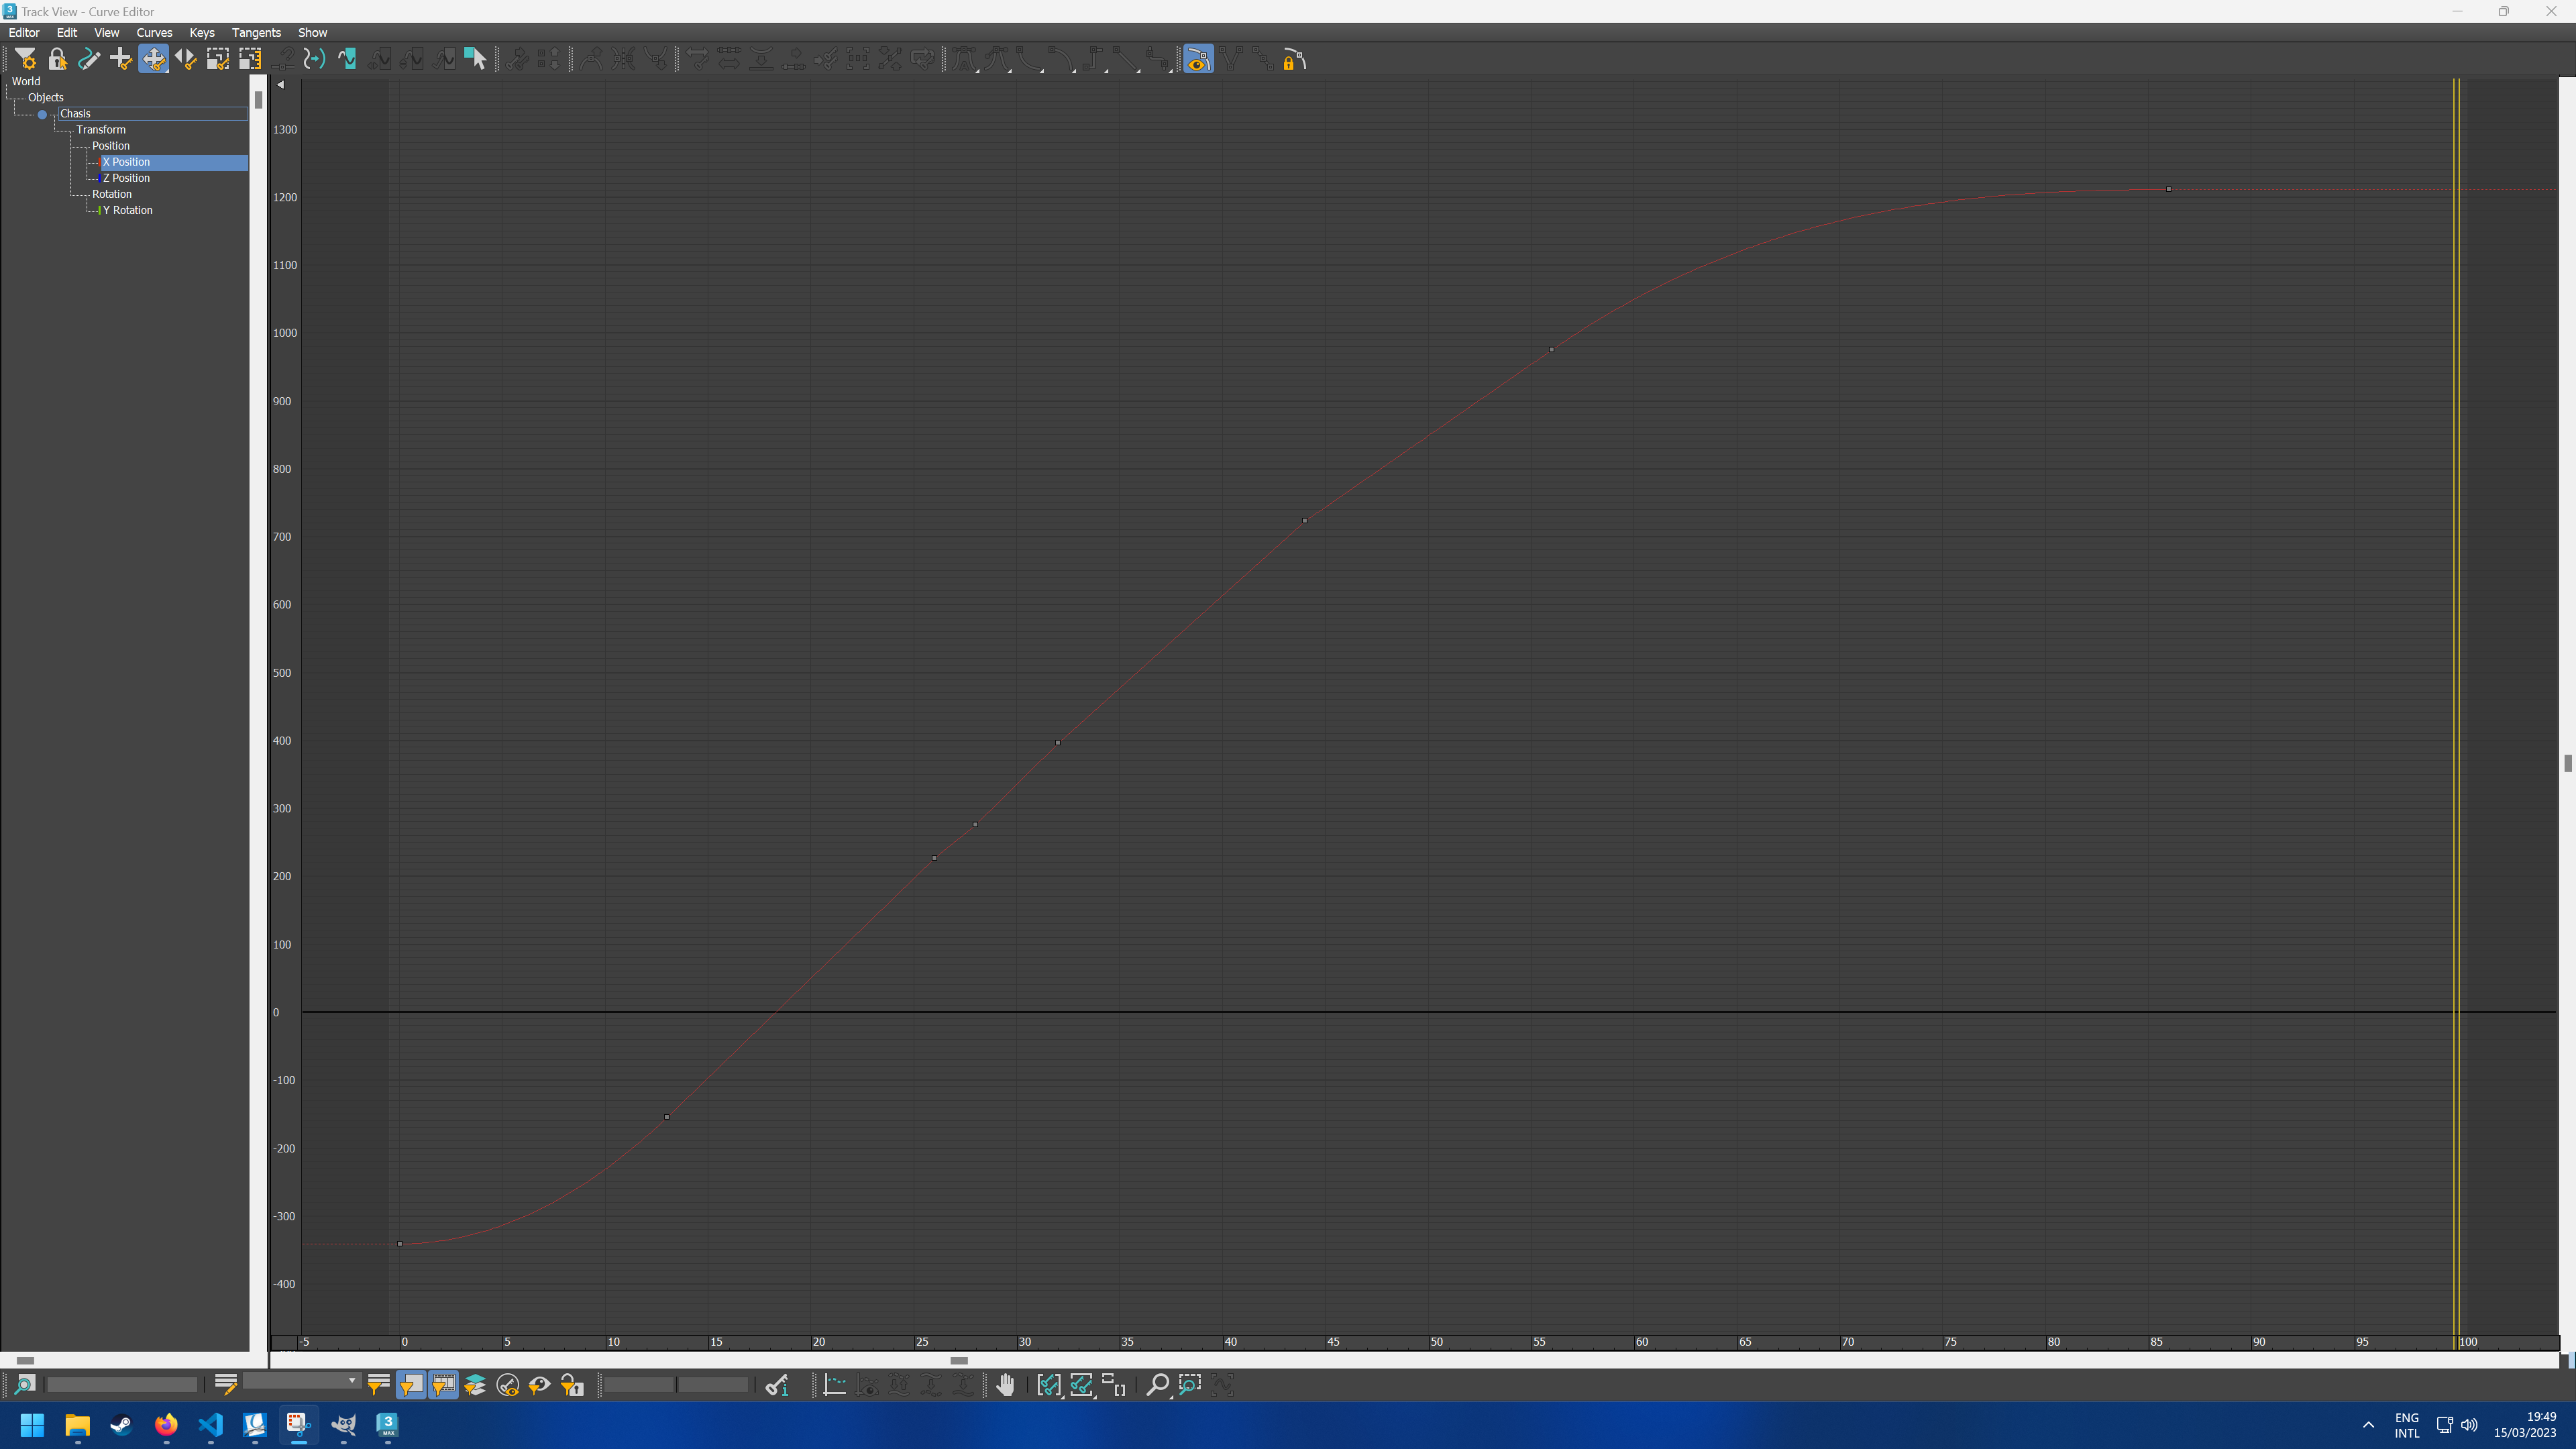
\includegraphics[width=\textwidth]{imagenes/Ejercicio2/curvas/red.png}
    \caption{Curva referente a la posición del vehículo en el eje X.}
 \end{figure}
 \begin{figure}[H]
    \centering
    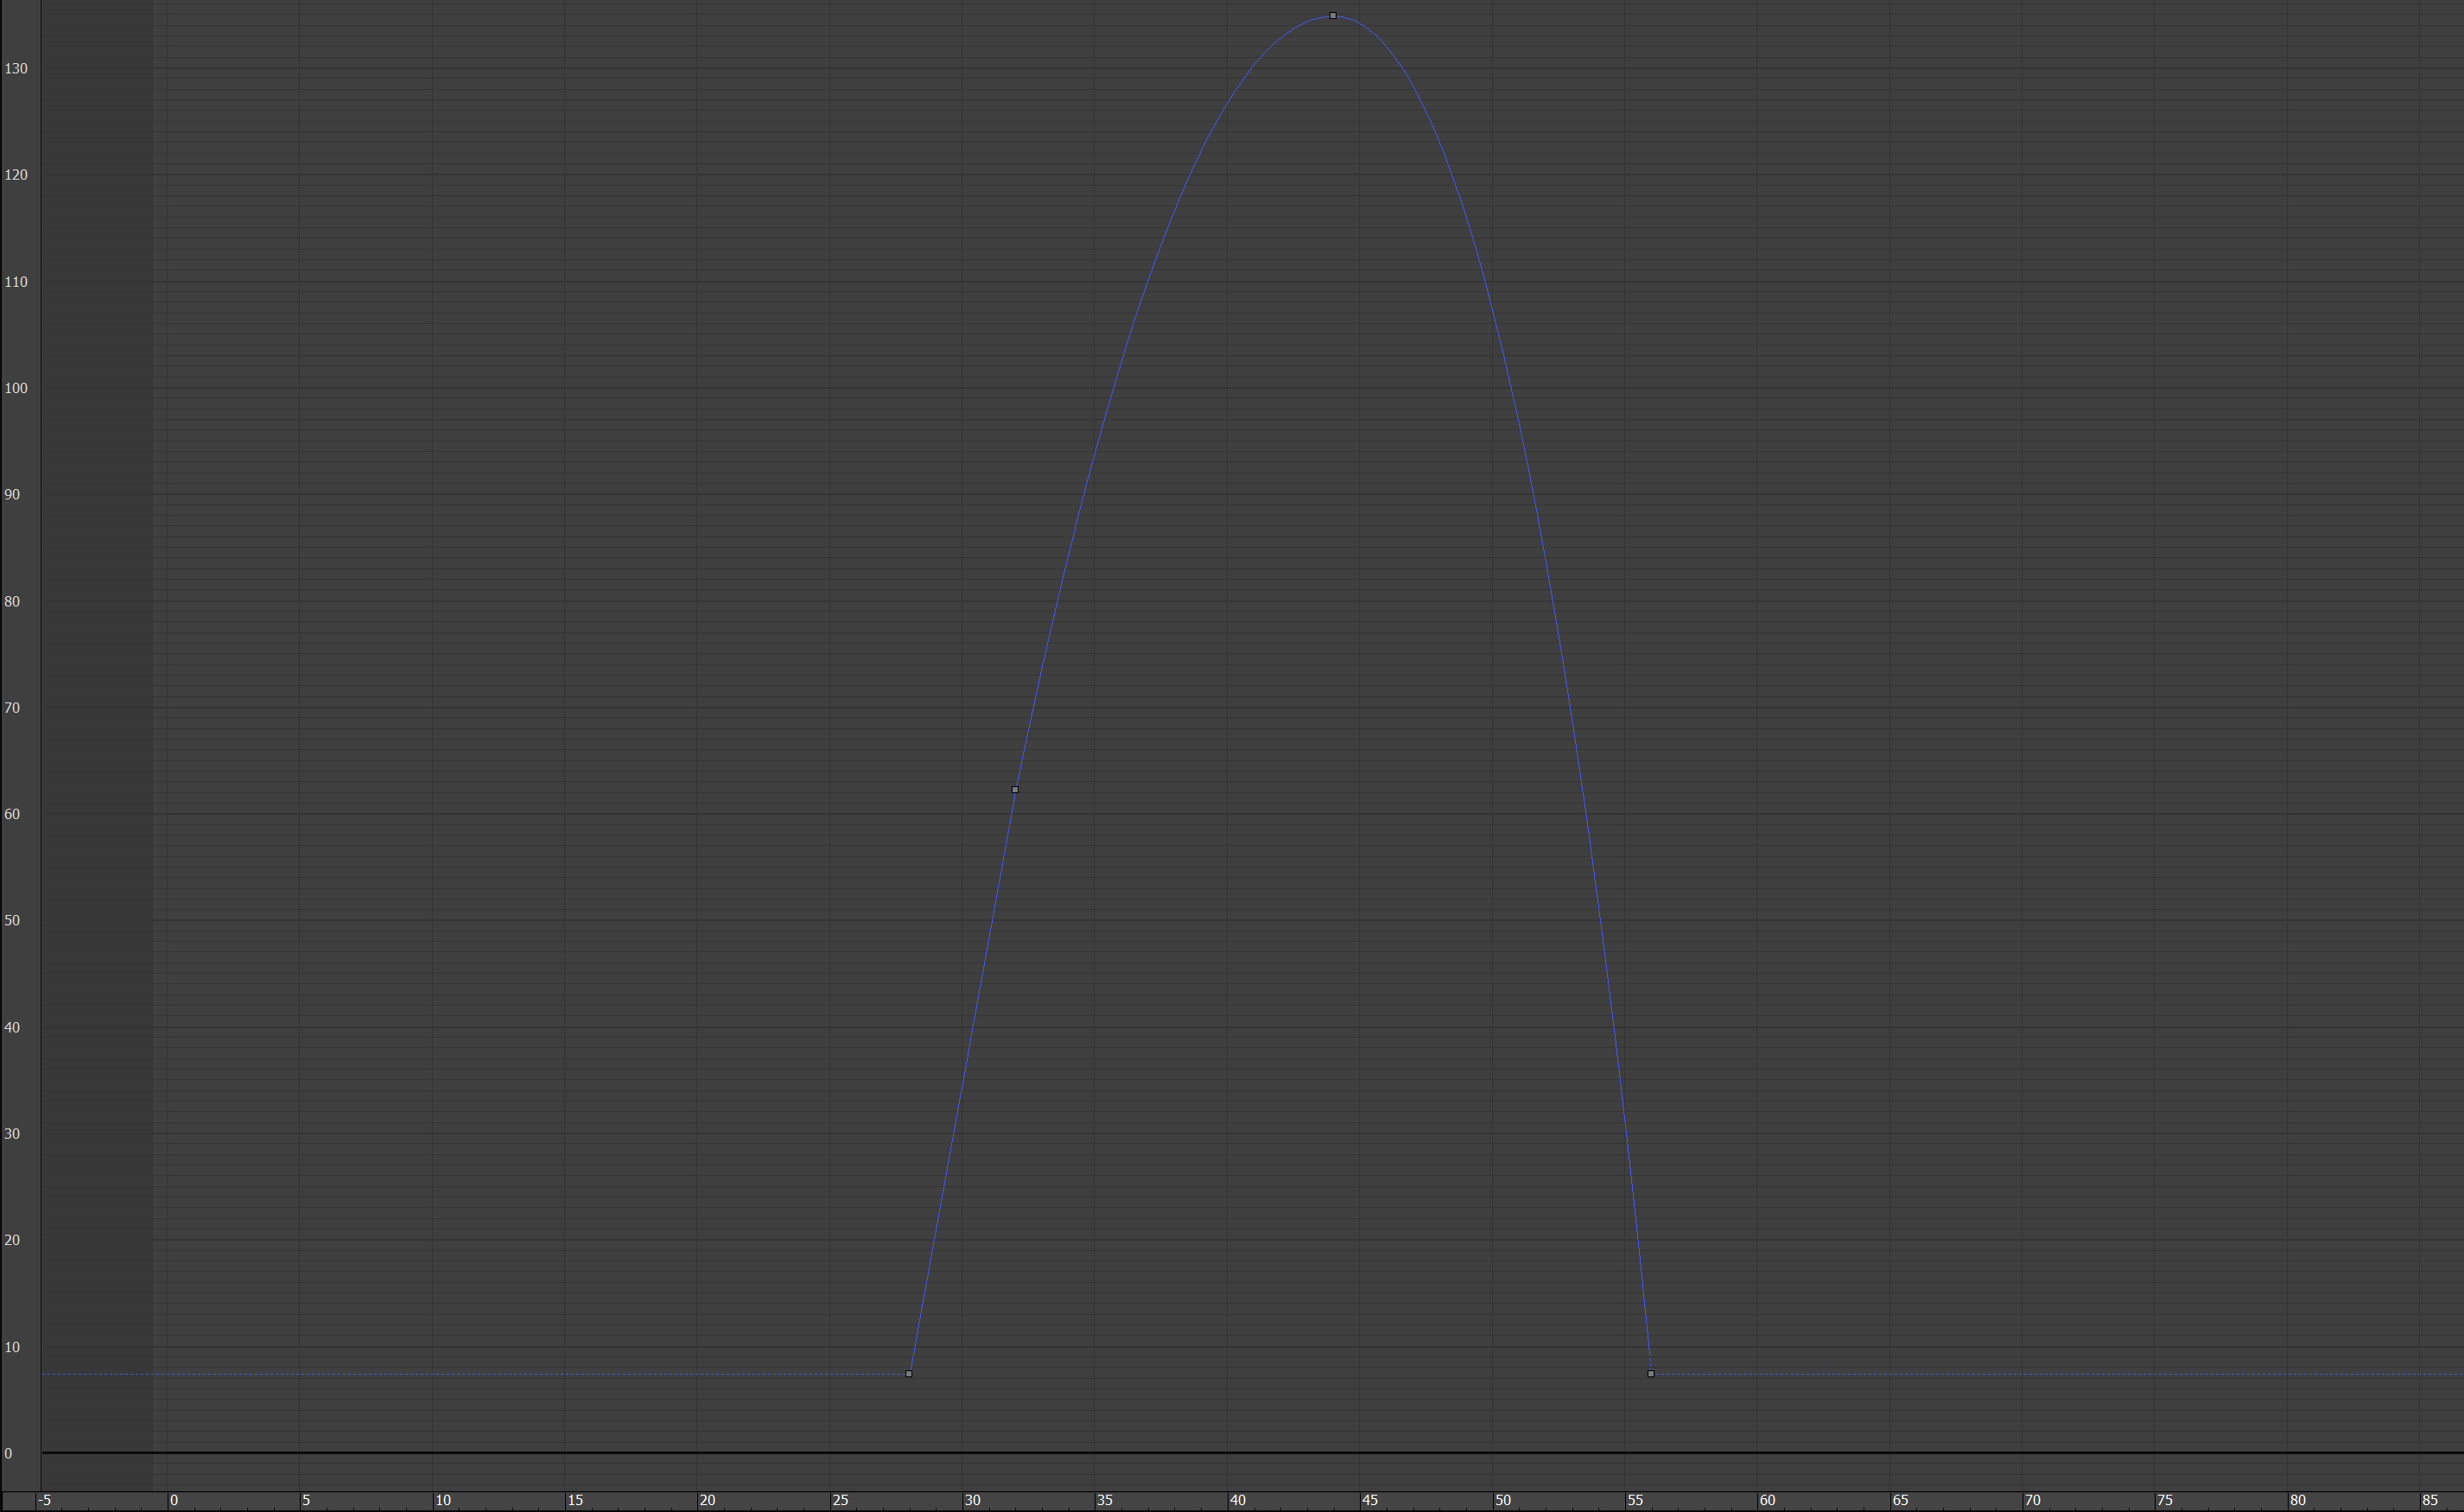
\includegraphics[width=\textwidth]{imagenes/Ejercicio2/curvas/blue.png}
    \caption{Curva referente a la posición del vehículo en el eje Z.}
 \end{figure}
 \begin{figure}[H]
    \centering
    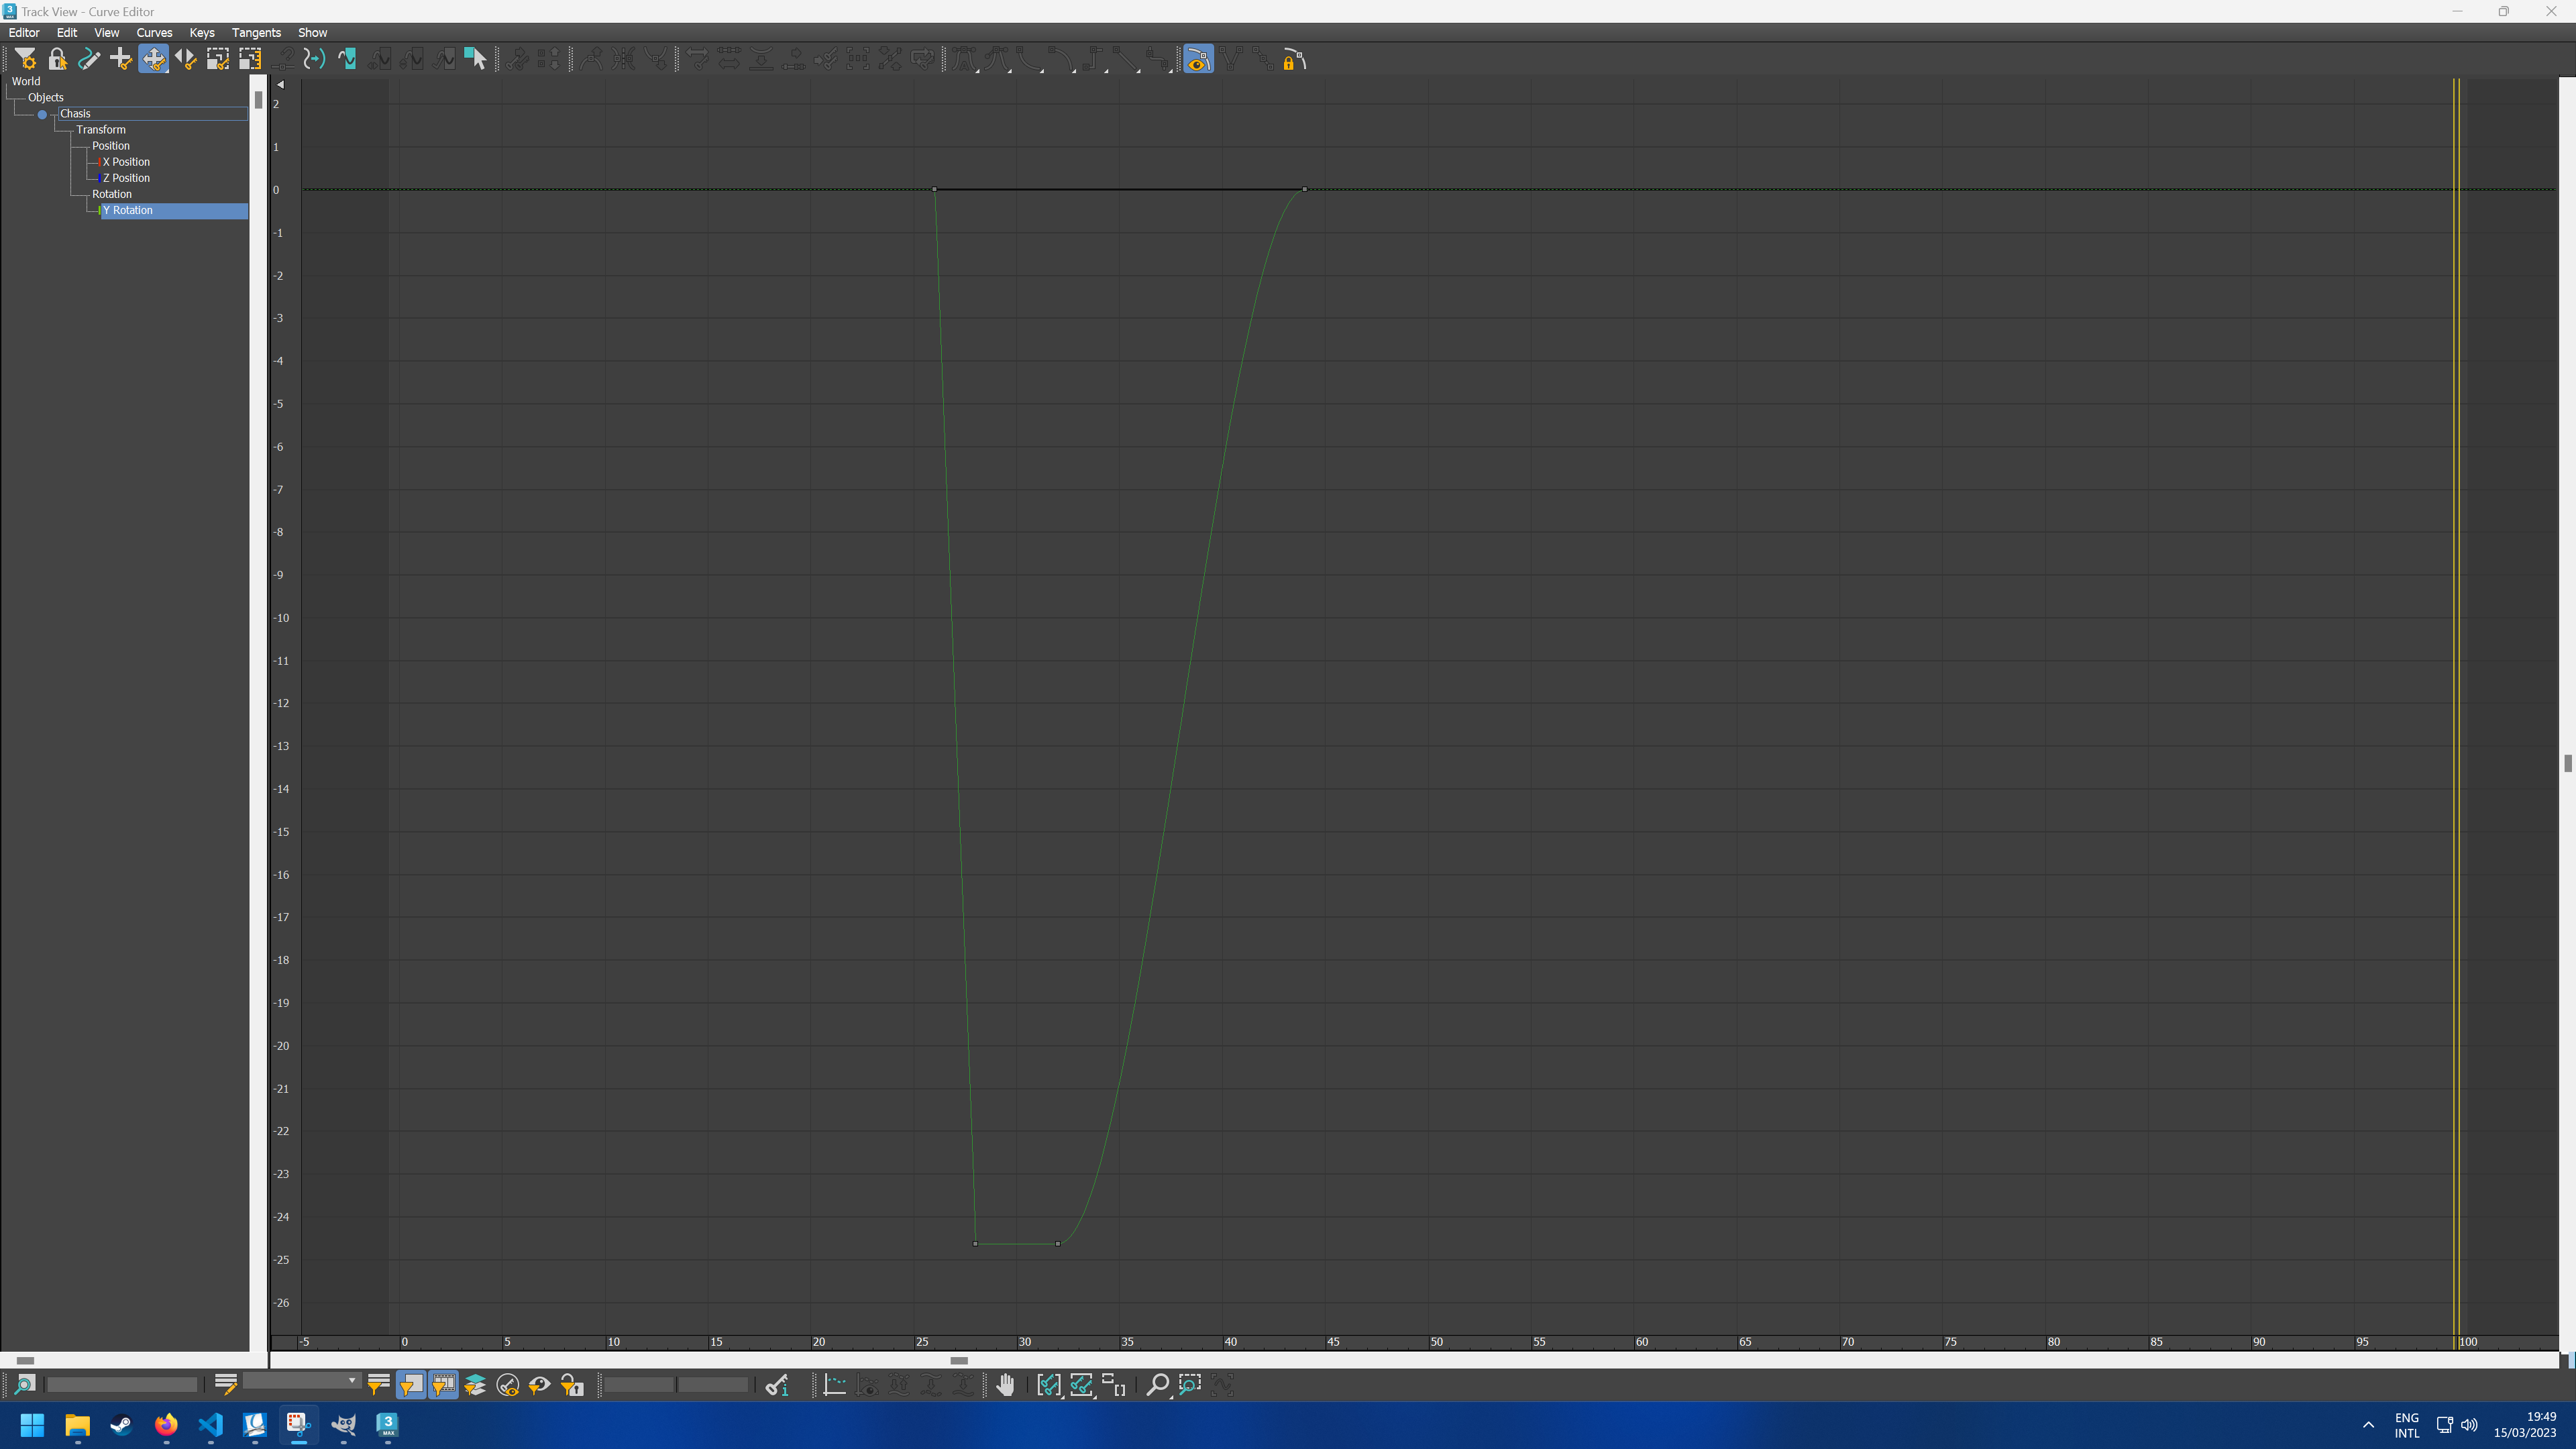
\includegraphics[width=\textwidth]{imagenes/Ejercicio2/curvas/green.png}
    \caption{Curva referente a la rotación del vehículo en el eje Y.}
 \end{figure}
% reescribir lo de abajo con chatgpt
Como se puede ver en la curva roja (posición en el eje X), al principio la curva tiene forma exponencial creciente, para simula la aceleración. A continuación, todo el trayecto se mantiene lineal, hasta llegar a la parte de frenado, donde tiene forma exponencial para que frene y se pare.

En cuanto a la curva de color azul (Posición en el eje Z), solo es usada para animar la subida de la rampa y la trayectoria que sigue el vehículo cuando sale despedido de la rampa. Entonces, la parte en la que sube a la rampa es lineal, con la misma pendiente que la rampa. Mientras que la animación de la trayectoria se hace con dos funciones exponenciales, para animar la fuerza que realiza la gravedad en la parte de la subida y para animar la aceleración de la gravedad en la bajada. Cabe destacar que, en este caso, la forma que tenga la curva será reflejada en la animación directamente; es decir, si la trayectoria se hubiera hecho lineal, el lanzamiento hubiese tenido forma triangular.

En cuanto a la curva verde (Rotación en el eje Y), es usada para rotar el vehículo en el cambio de pendiente de la subida de la rampa y cuando se endereza durante el lanzamiento del vehículo.
% fin rescritura

\section{Ejercicio 3 - Pelota botando}

En este ejercicio se pide animar una pelota que rebota varias veces sobre una mesa y que finalmente se cae al suelo. 

La mesa la he realizado usando 5 cubos: uno grande para el tablero y otros 4 del mismo tamaño para hacer las patas. Además, la jerarquía utilizada ha sido de dejar como padre al tablero y como hijos las patas.

%rescribir
En cuanto a la animacion, he utilizado un factor de 2 para la altura del rebote y para la distancia recorrida entre rebotes; es decir, que en cada salto su altura y distancia de divide a la mitad. La única parte en la que no se sigue esto es en el primer lanzamiento horizontal, ya que probando a seguir este factor el resultado era menos realista, pero la altura sí lo respeta, como pedía el ejercicio. Esta aniamción la he realizado usando 10 \textit{keyframes}, que son:

\begin{enumerate}
    \item Instante 0: La pelota se encuentra en el aire, lista para ser lanzada a la mesa.
    \item Instante 15: La pelota ha tocado la mesa por primera vez.
    \item Instantes 25, 42, 54: La pelota ha rebotado y se encuentra en el aire.
    \item Instantes 35, 49, 59: La pelota ha tocado de nuevo el tablero de la mesa.
    \item Instante 71: La pelota se encuentra en el borde de la mesa, justo antes de que se caiga al suelo.
    \item Instante 84: La pelota ha caido y se encuentra en el suelo.
\end{enumerate}

% imagenes con los keyframes
\begin{figure}[H]
    \centering
    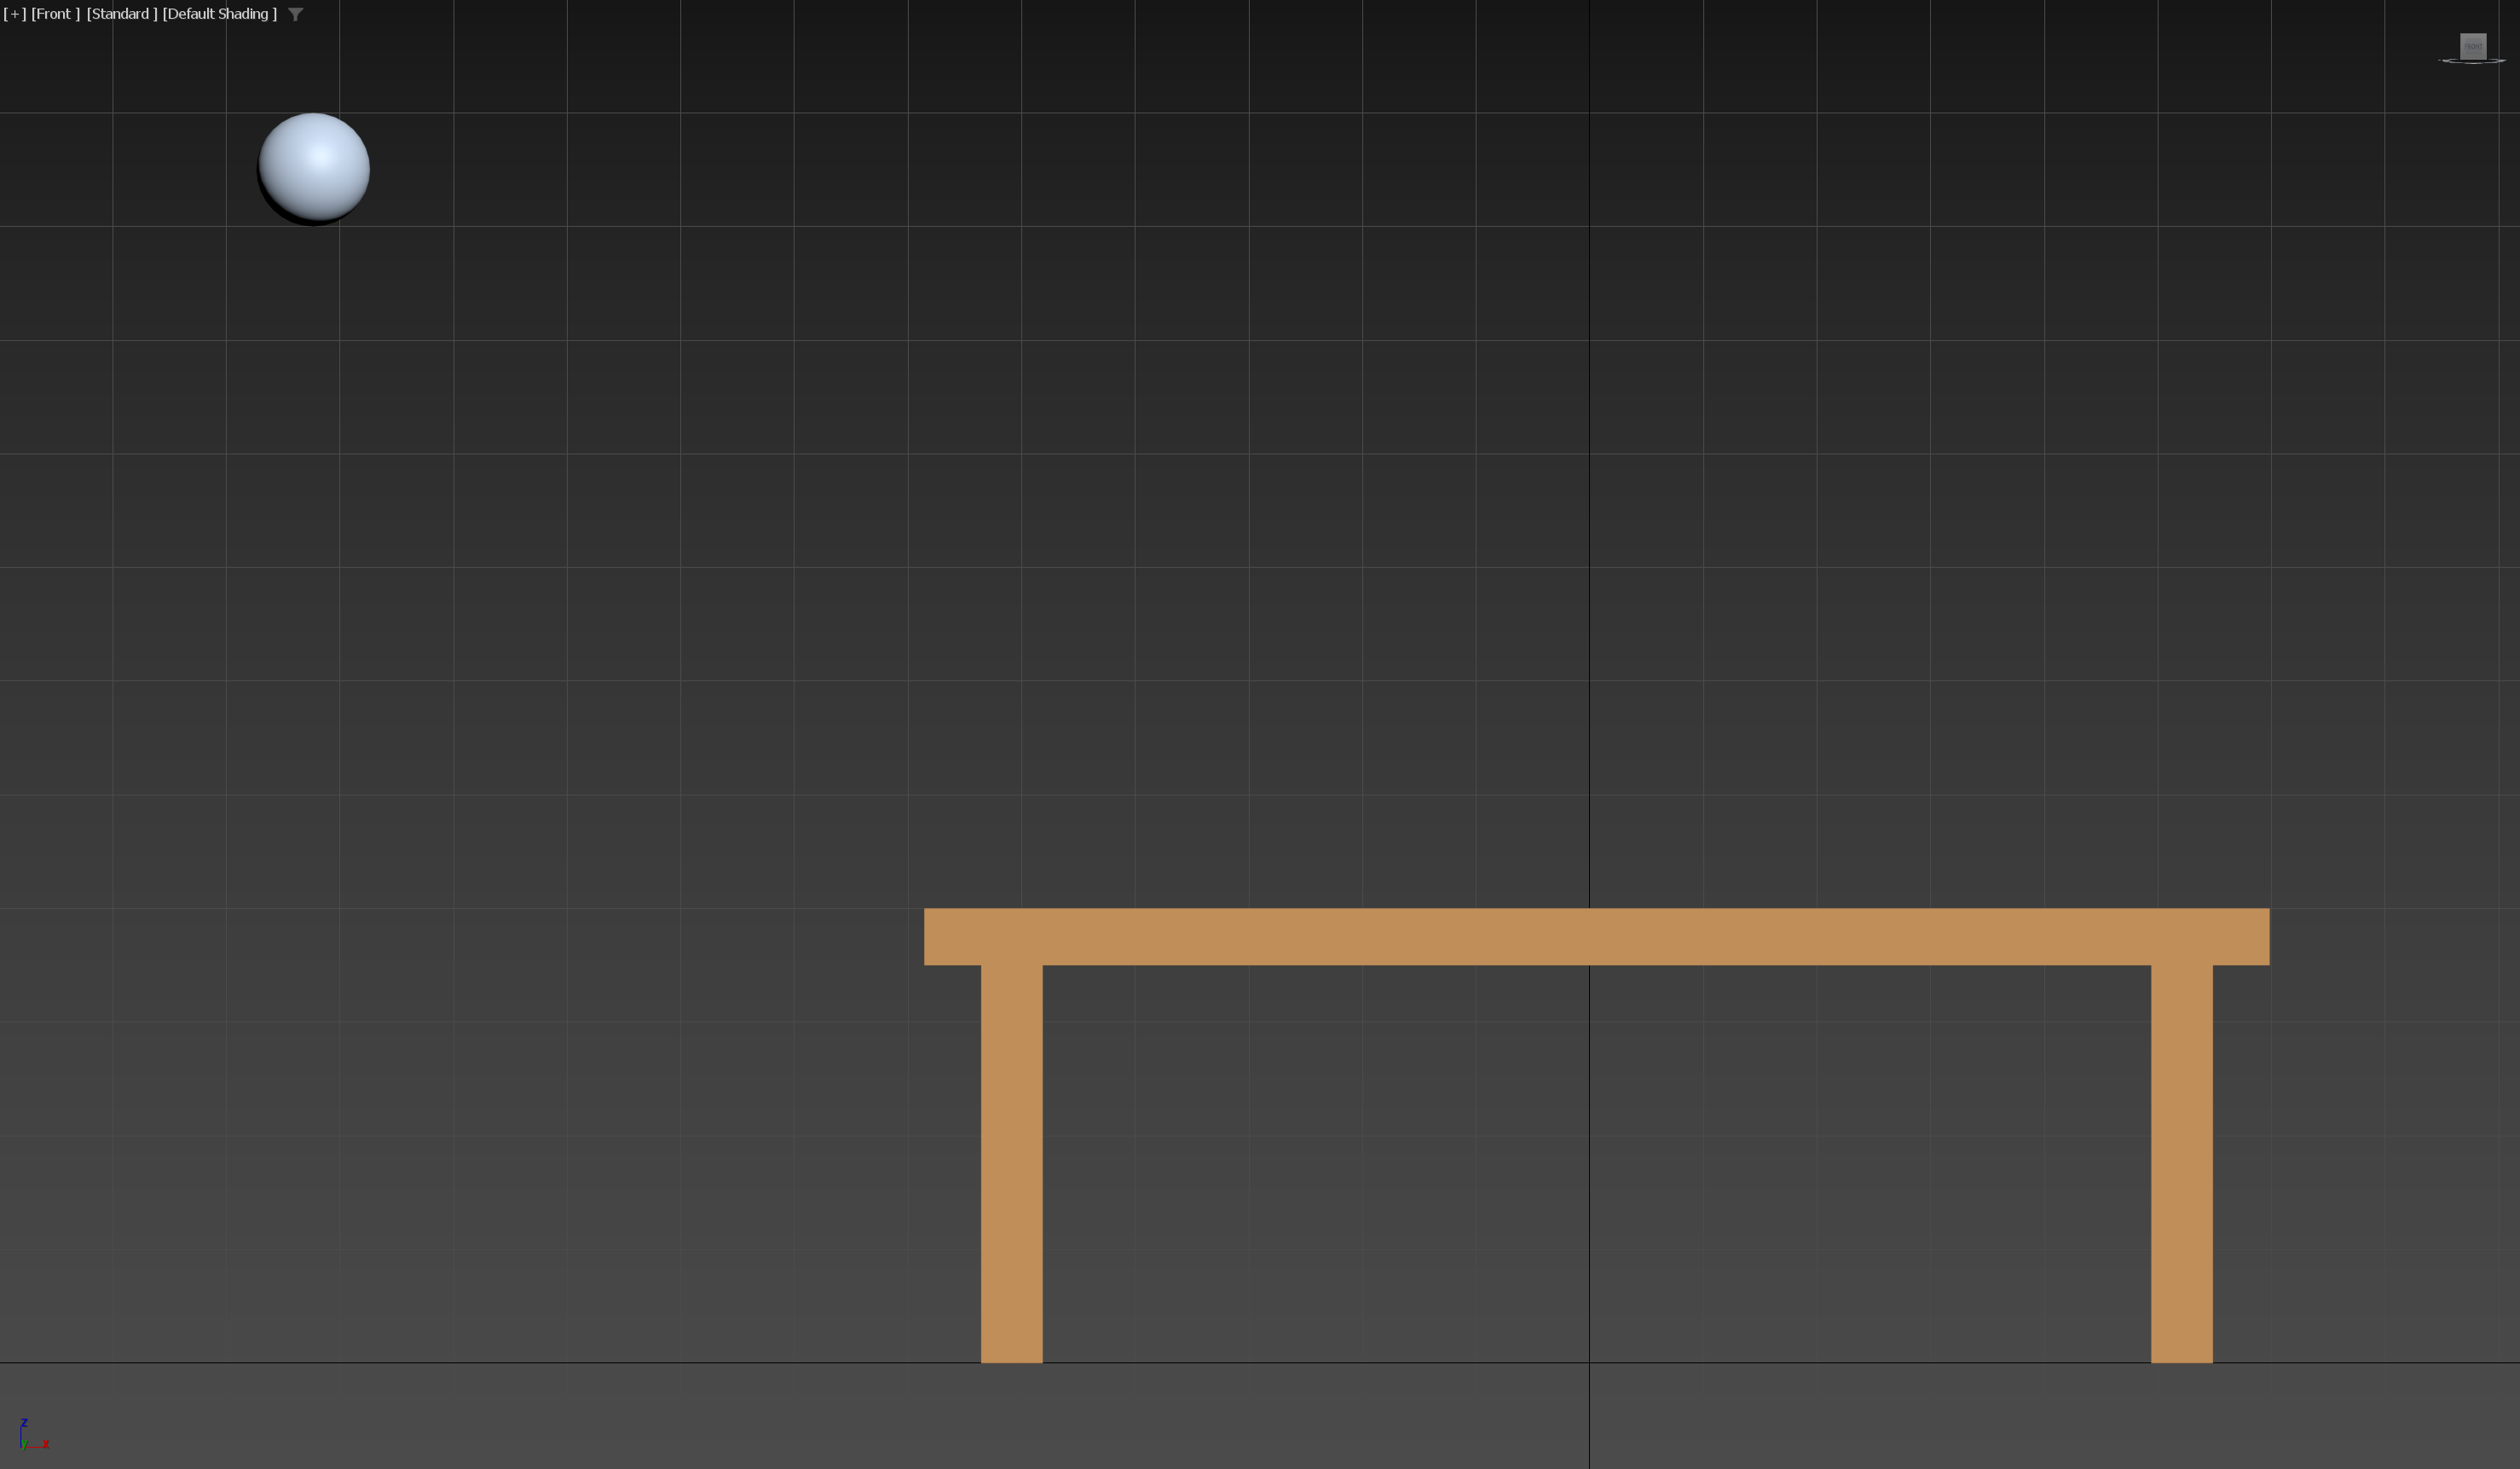
\includegraphics[width=\textwidth]{imagenes/Ejercicio3/keyframes/0.png}
    \caption{Pelota en el instante 0.}
\end{figure}
\begin{figure}[H]
    \centering
    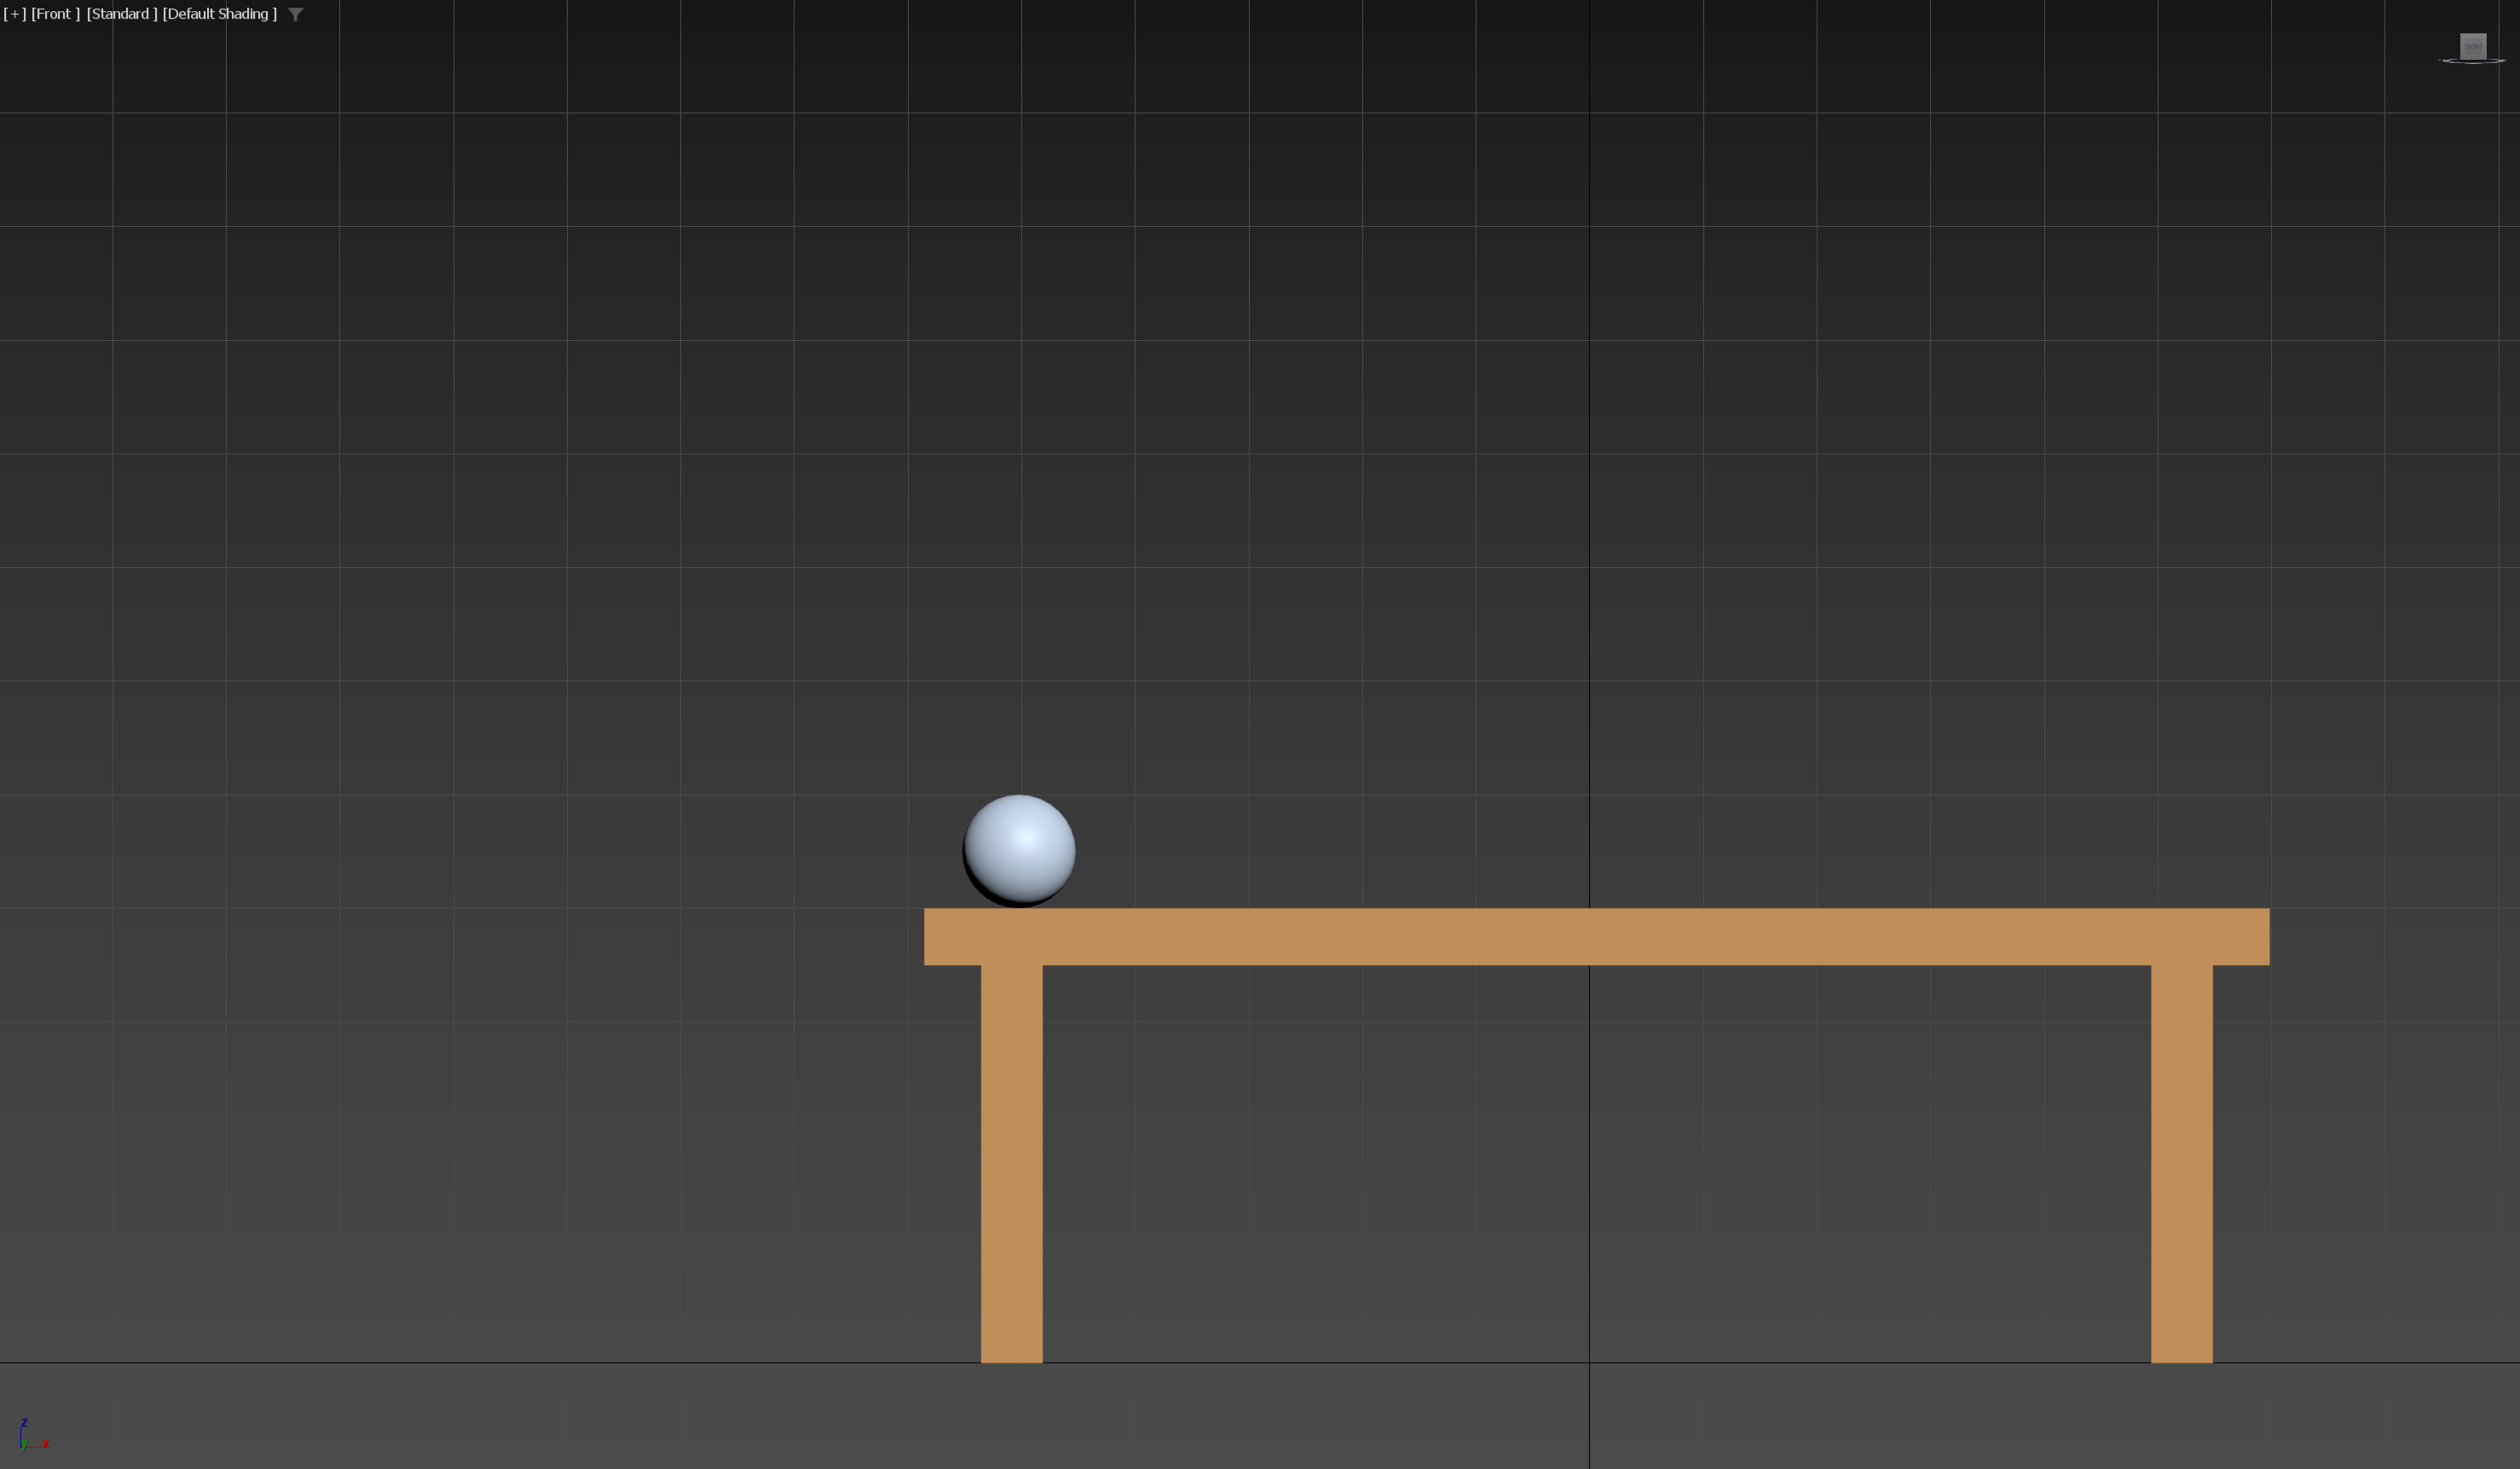
\includegraphics[width=\textwidth]{imagenes/Ejercicio3/keyframes/15.png}
    \caption{Pelota en el instante 15.}
\end{figure}
\begin{figure}[H]
    \centering
    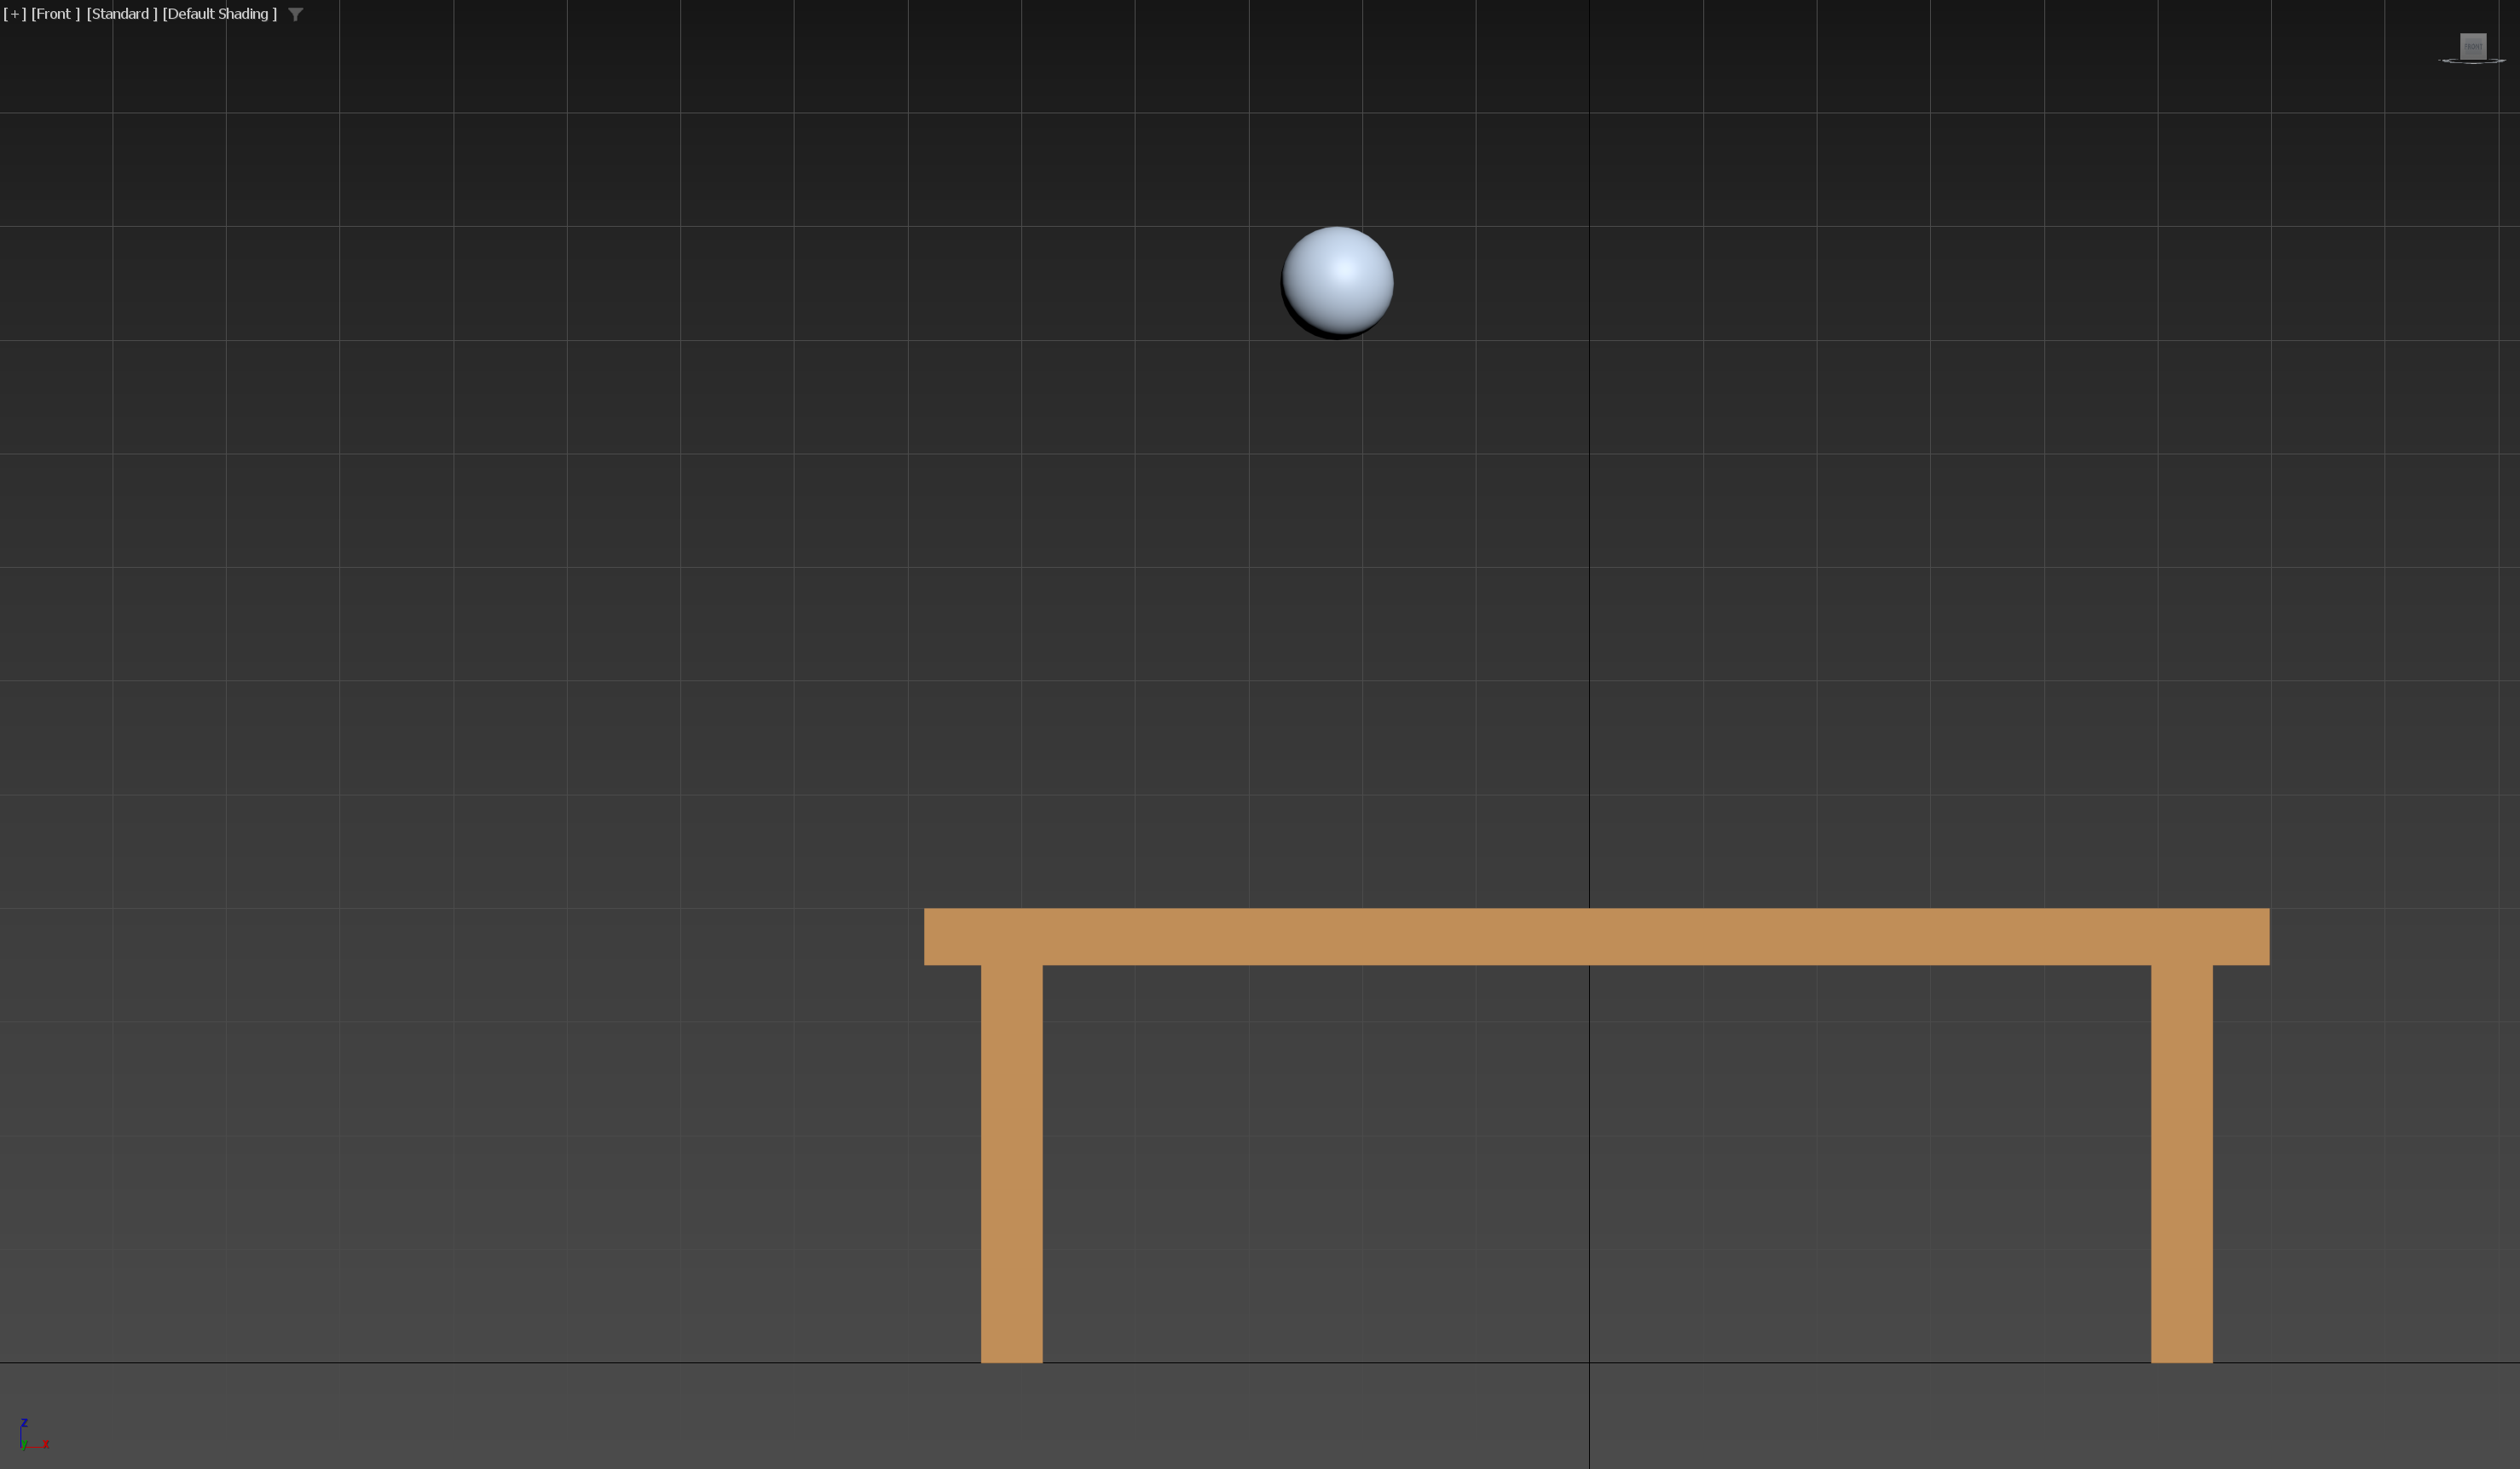
\includegraphics[width=\textwidth]{imagenes/Ejercicio3/keyframes/25.png}
    \caption{Pelota en el instante 25.}
\end{figure}
\begin{figure}[H]
    \centering
    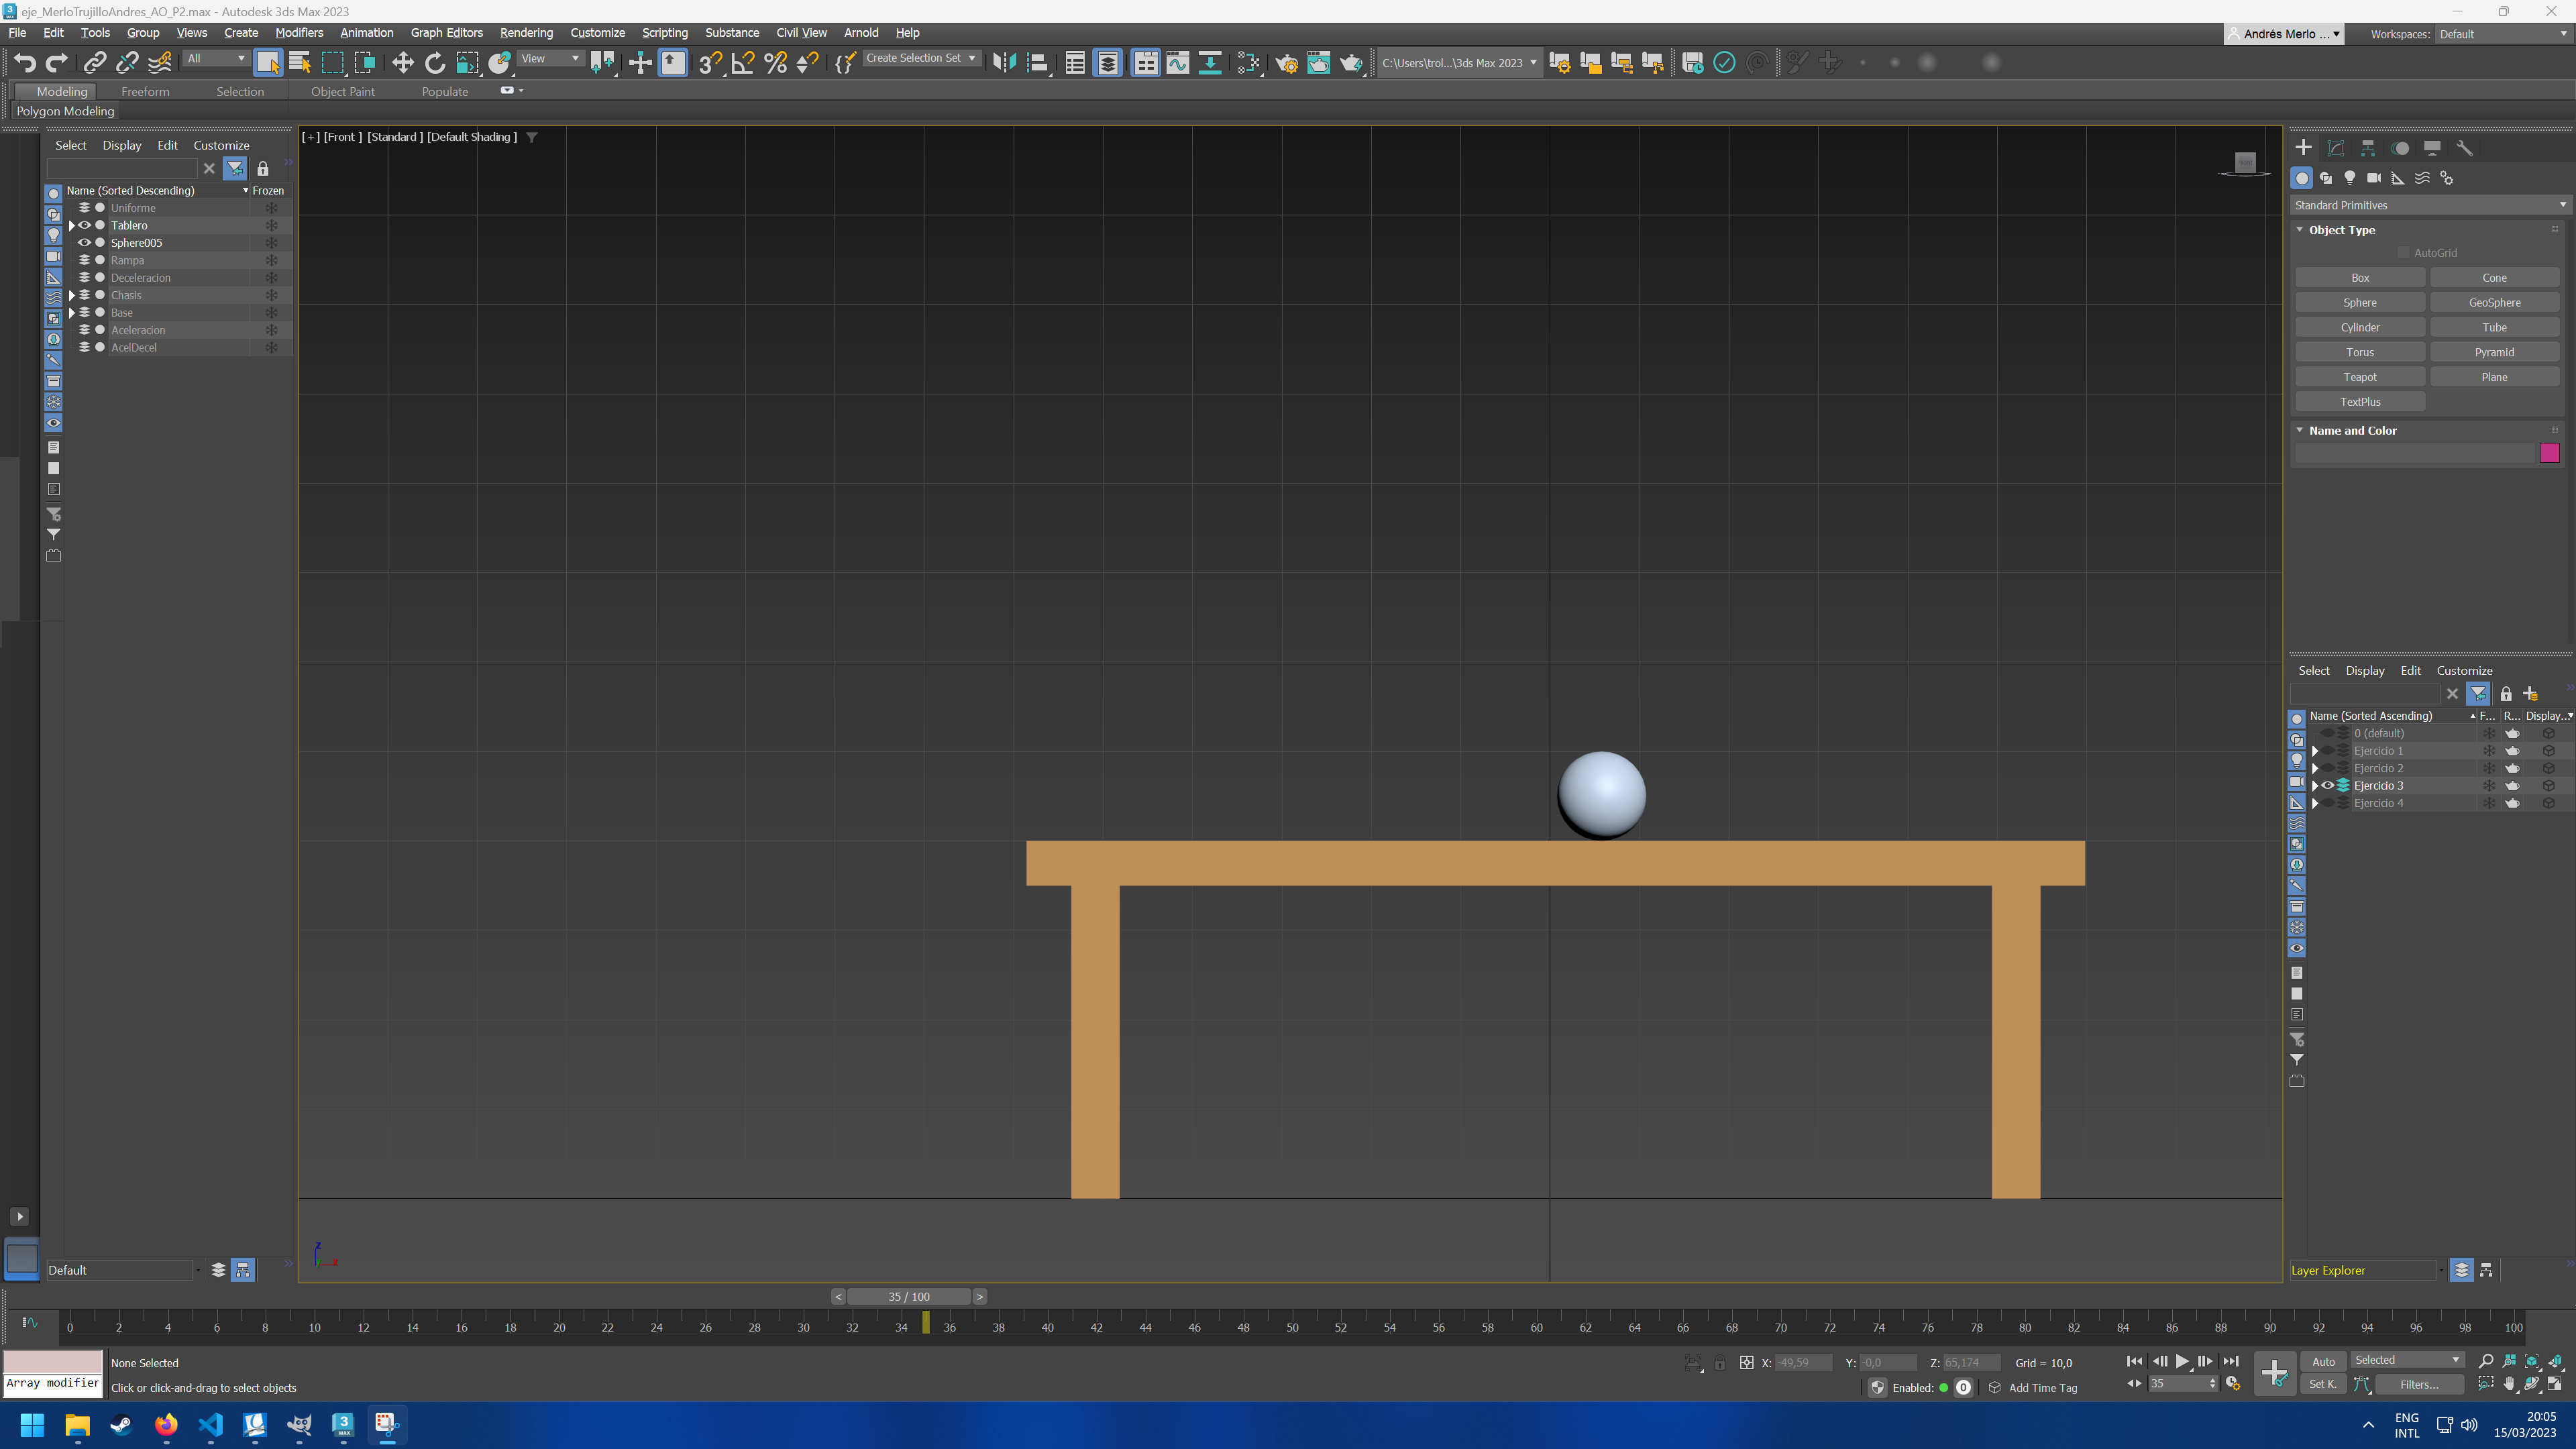
\includegraphics[width=\textwidth]{imagenes/Ejercicio3/keyframes/35.png}
    \caption{Pelota en el instante 35.}
\end{figure}
\begin{figure}[H]
    \centering
    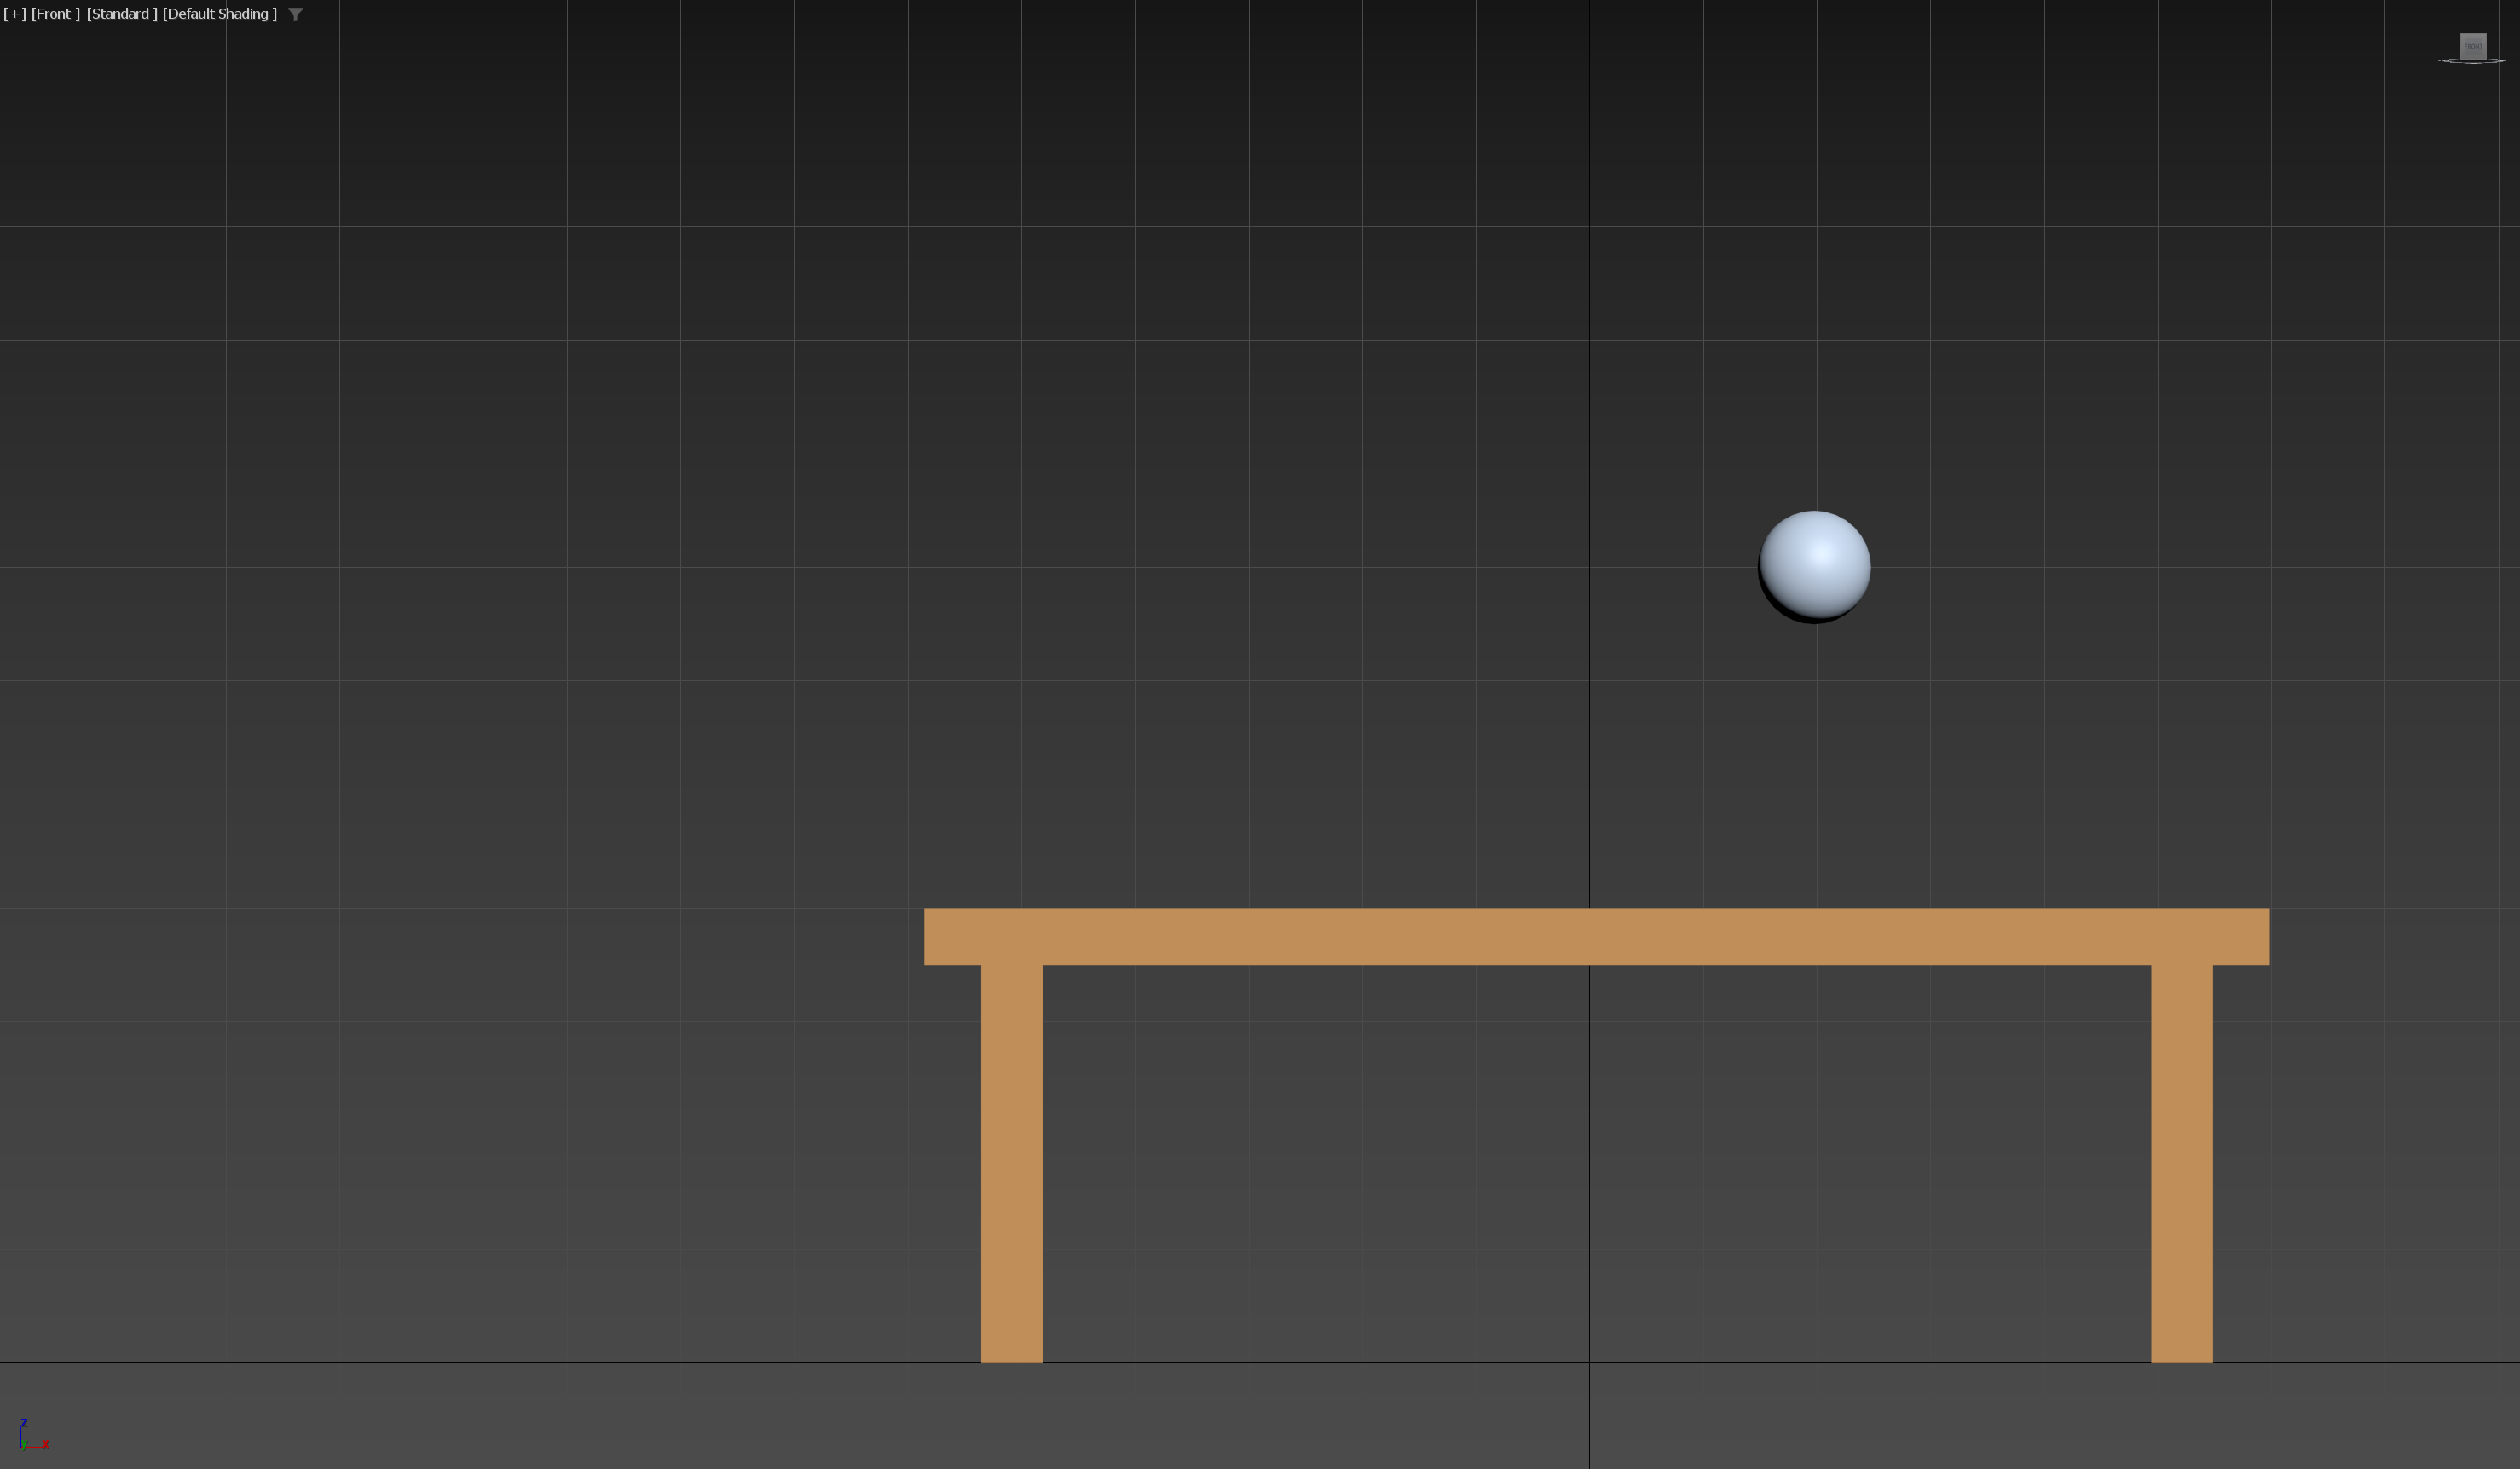
\includegraphics[width=\textwidth]{imagenes/Ejercicio3/keyframes/42.png}
    \caption{Pelota en el instante 42.}
\end{figure}
\begin{figure}[H]
    \centering
    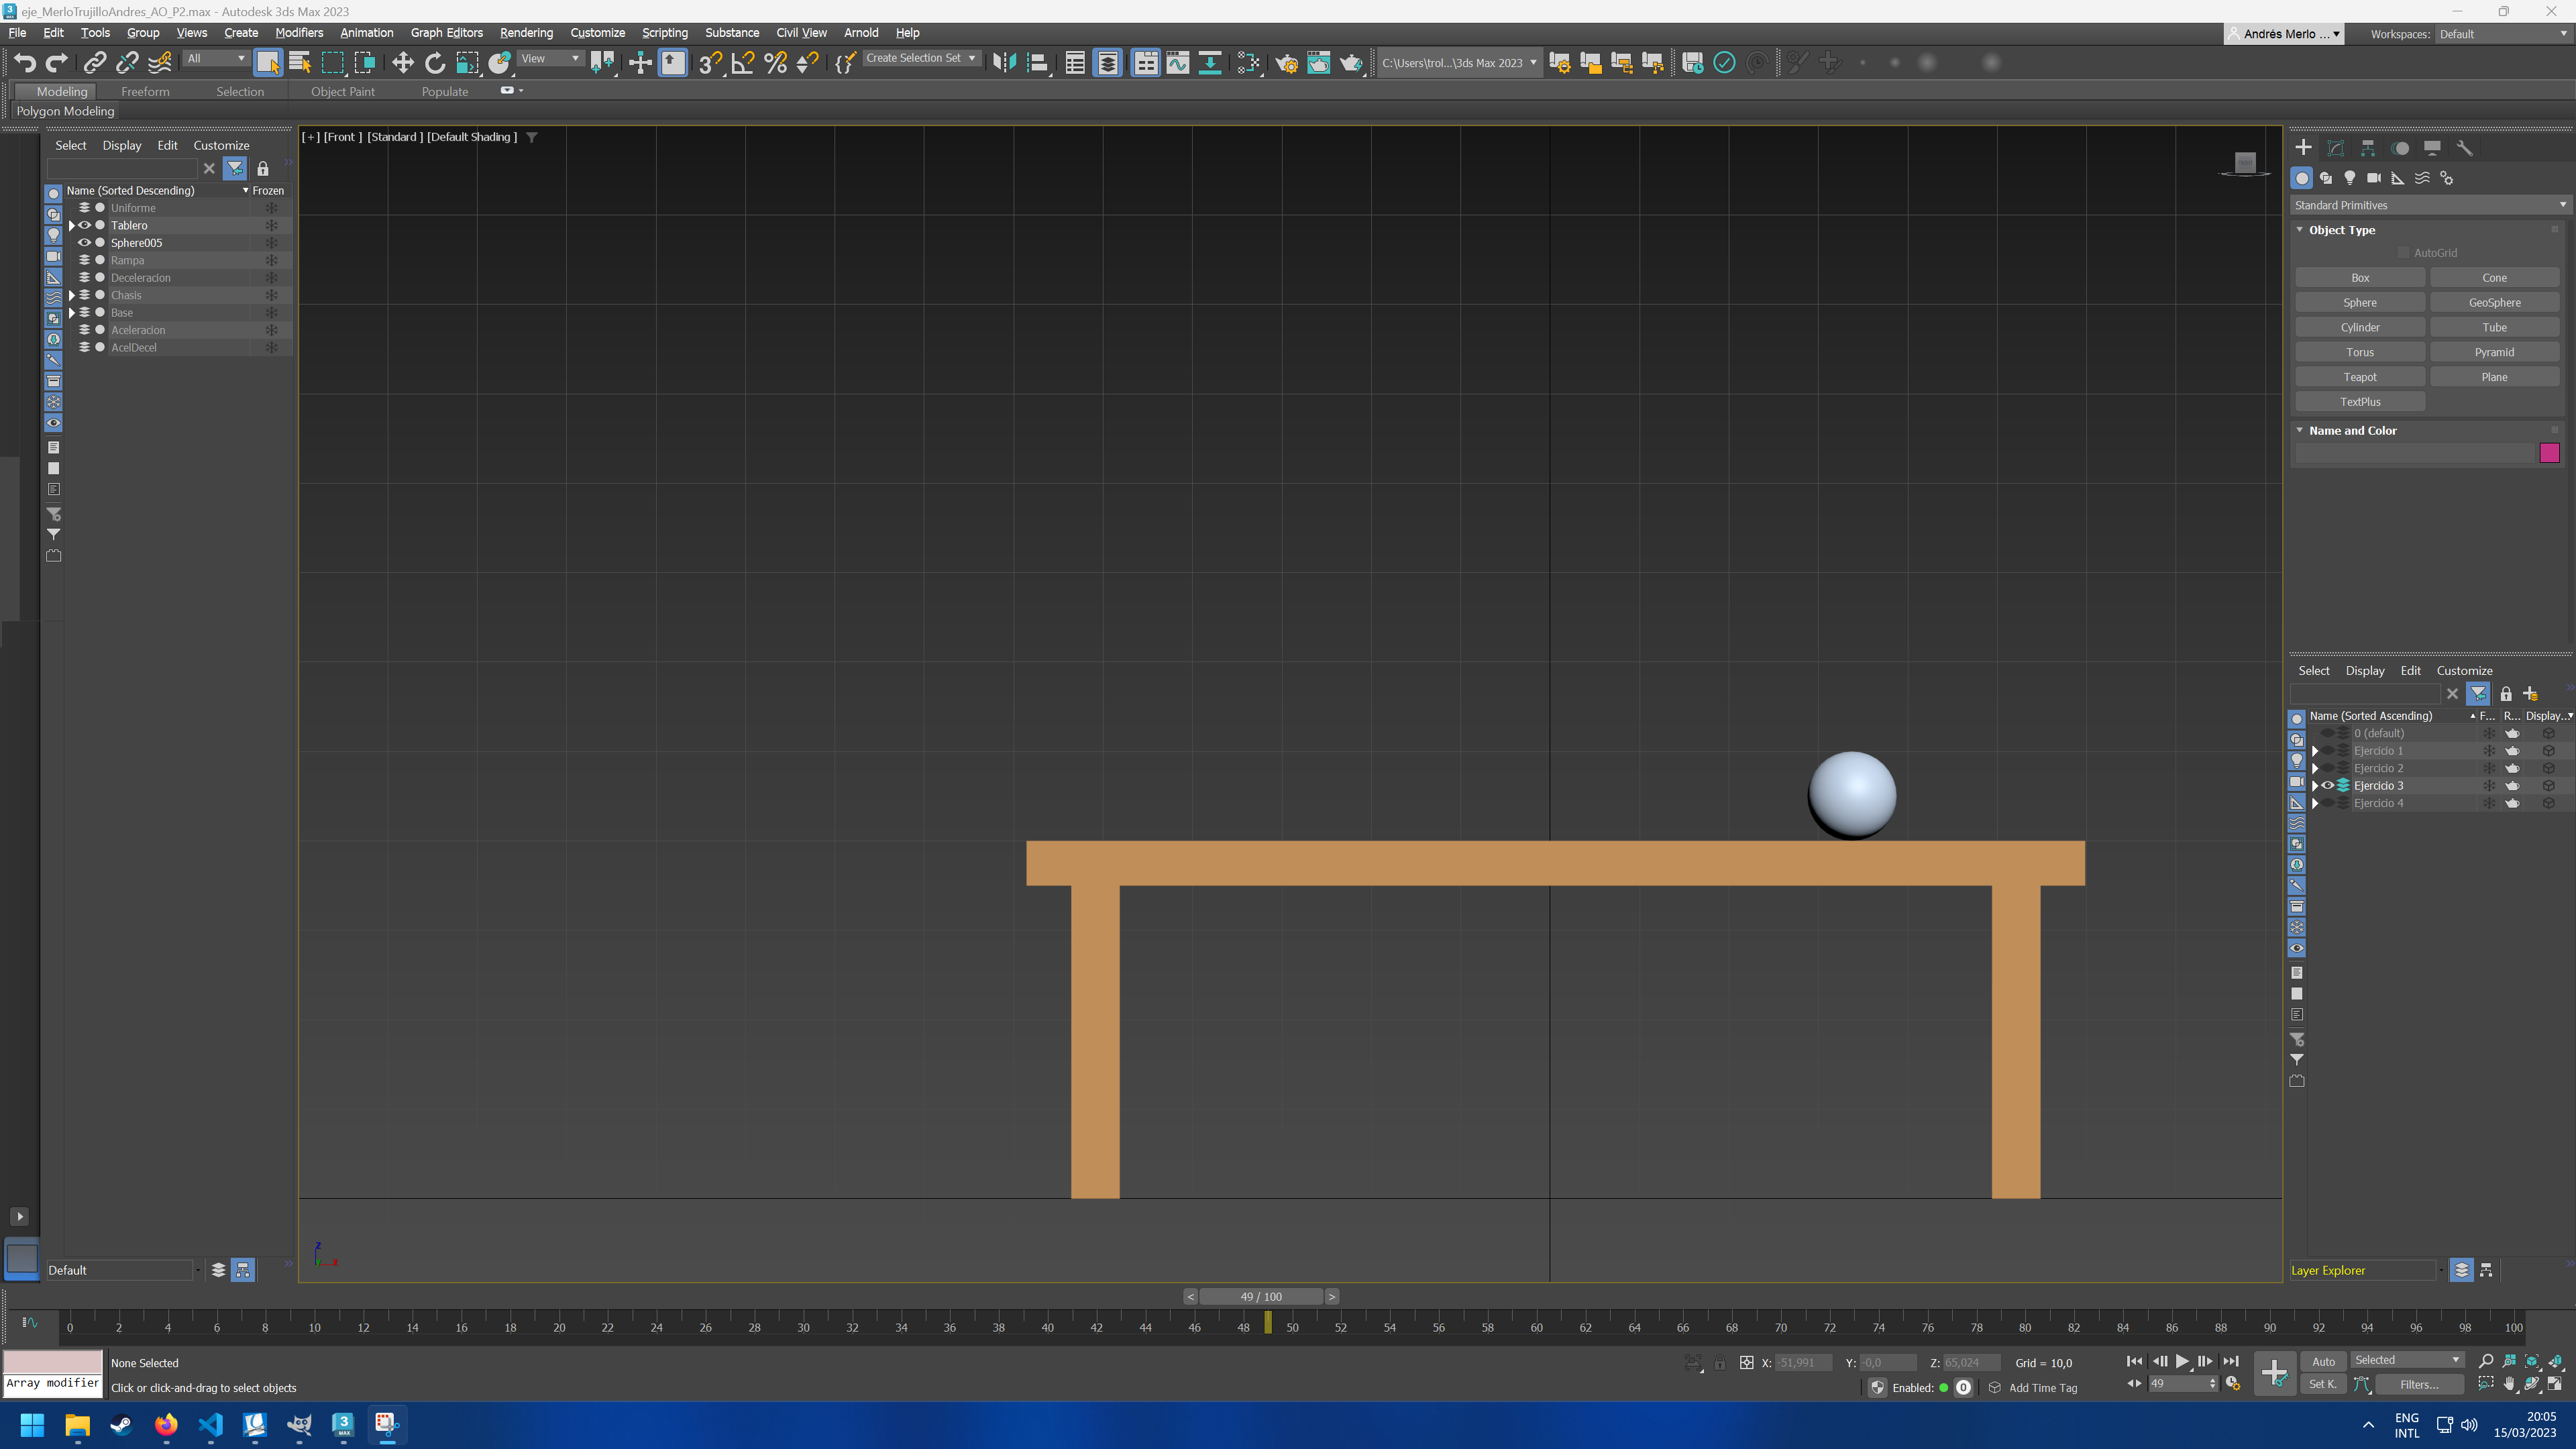
\includegraphics[width=\textwidth]{imagenes/Ejercicio3/keyframes/49.png}
    \caption{Pelota en el instante 49.}
\end{figure}
\begin{figure}[H]
    \centering
    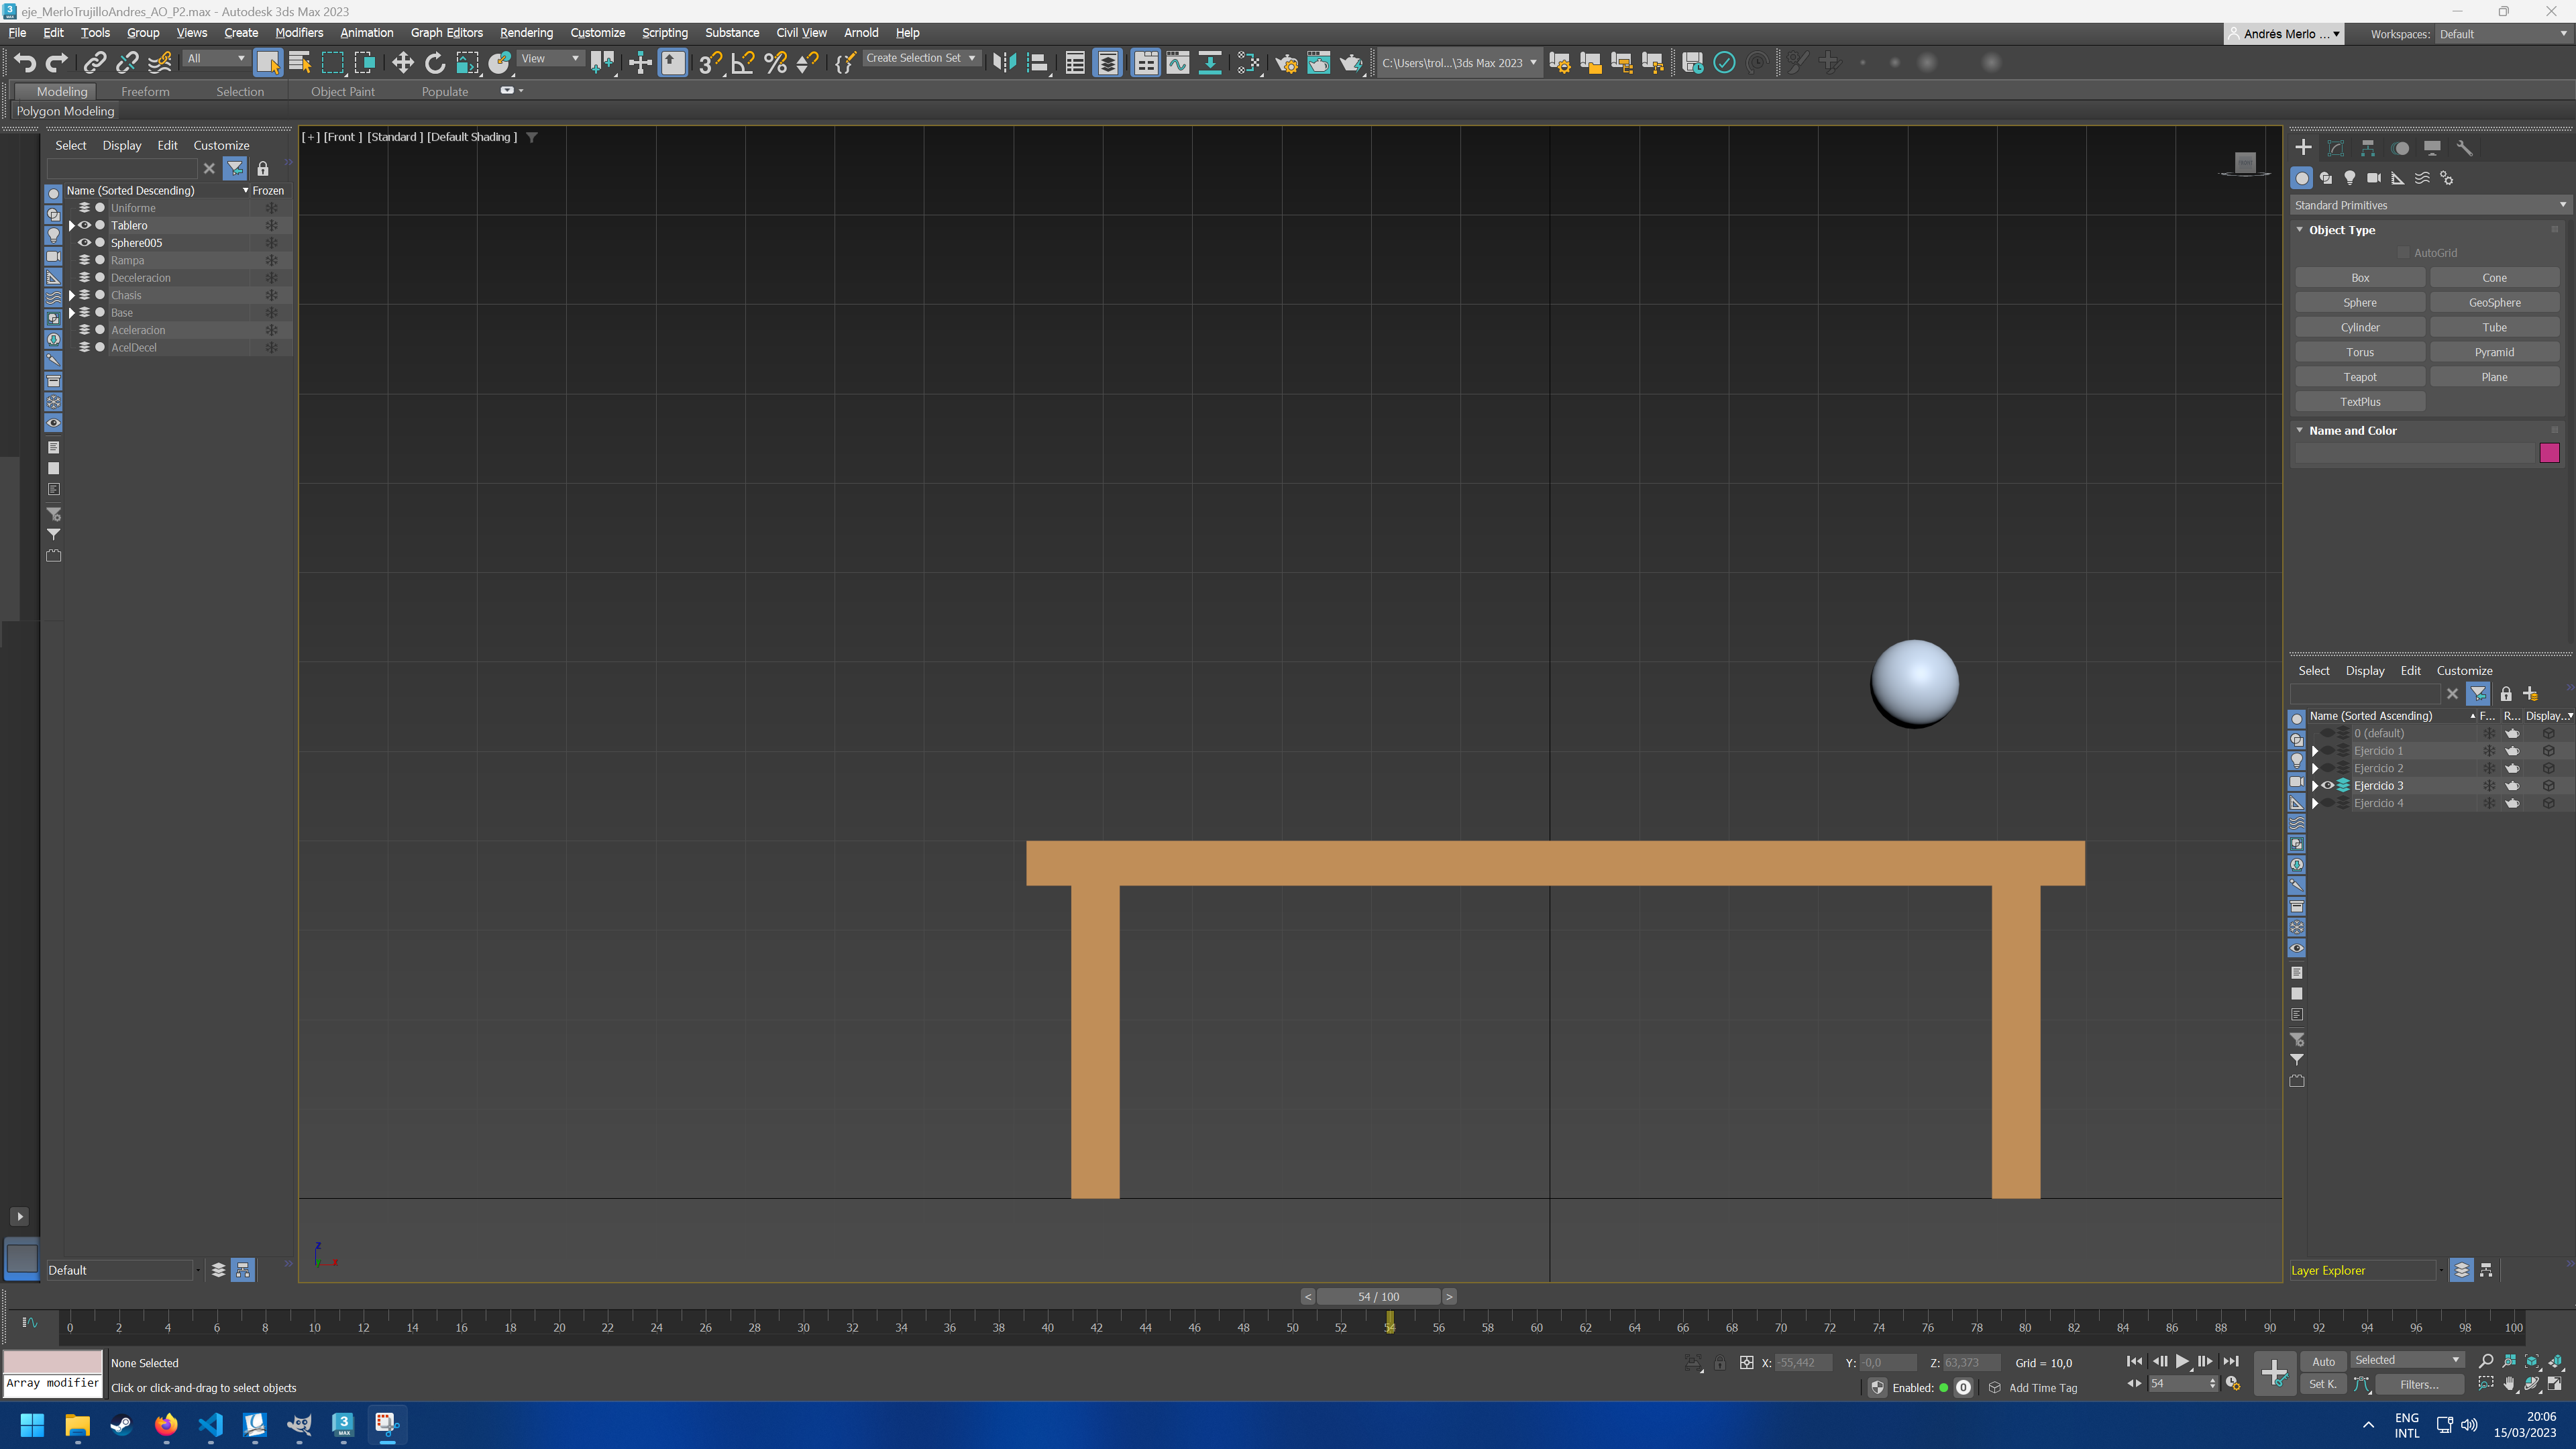
\includegraphics[width=\textwidth]{imagenes/Ejercicio3/keyframes/54.png}
    \caption{Pelota en el instante 54.}
\end{figure}
\begin{figure}[H]
    \centering
    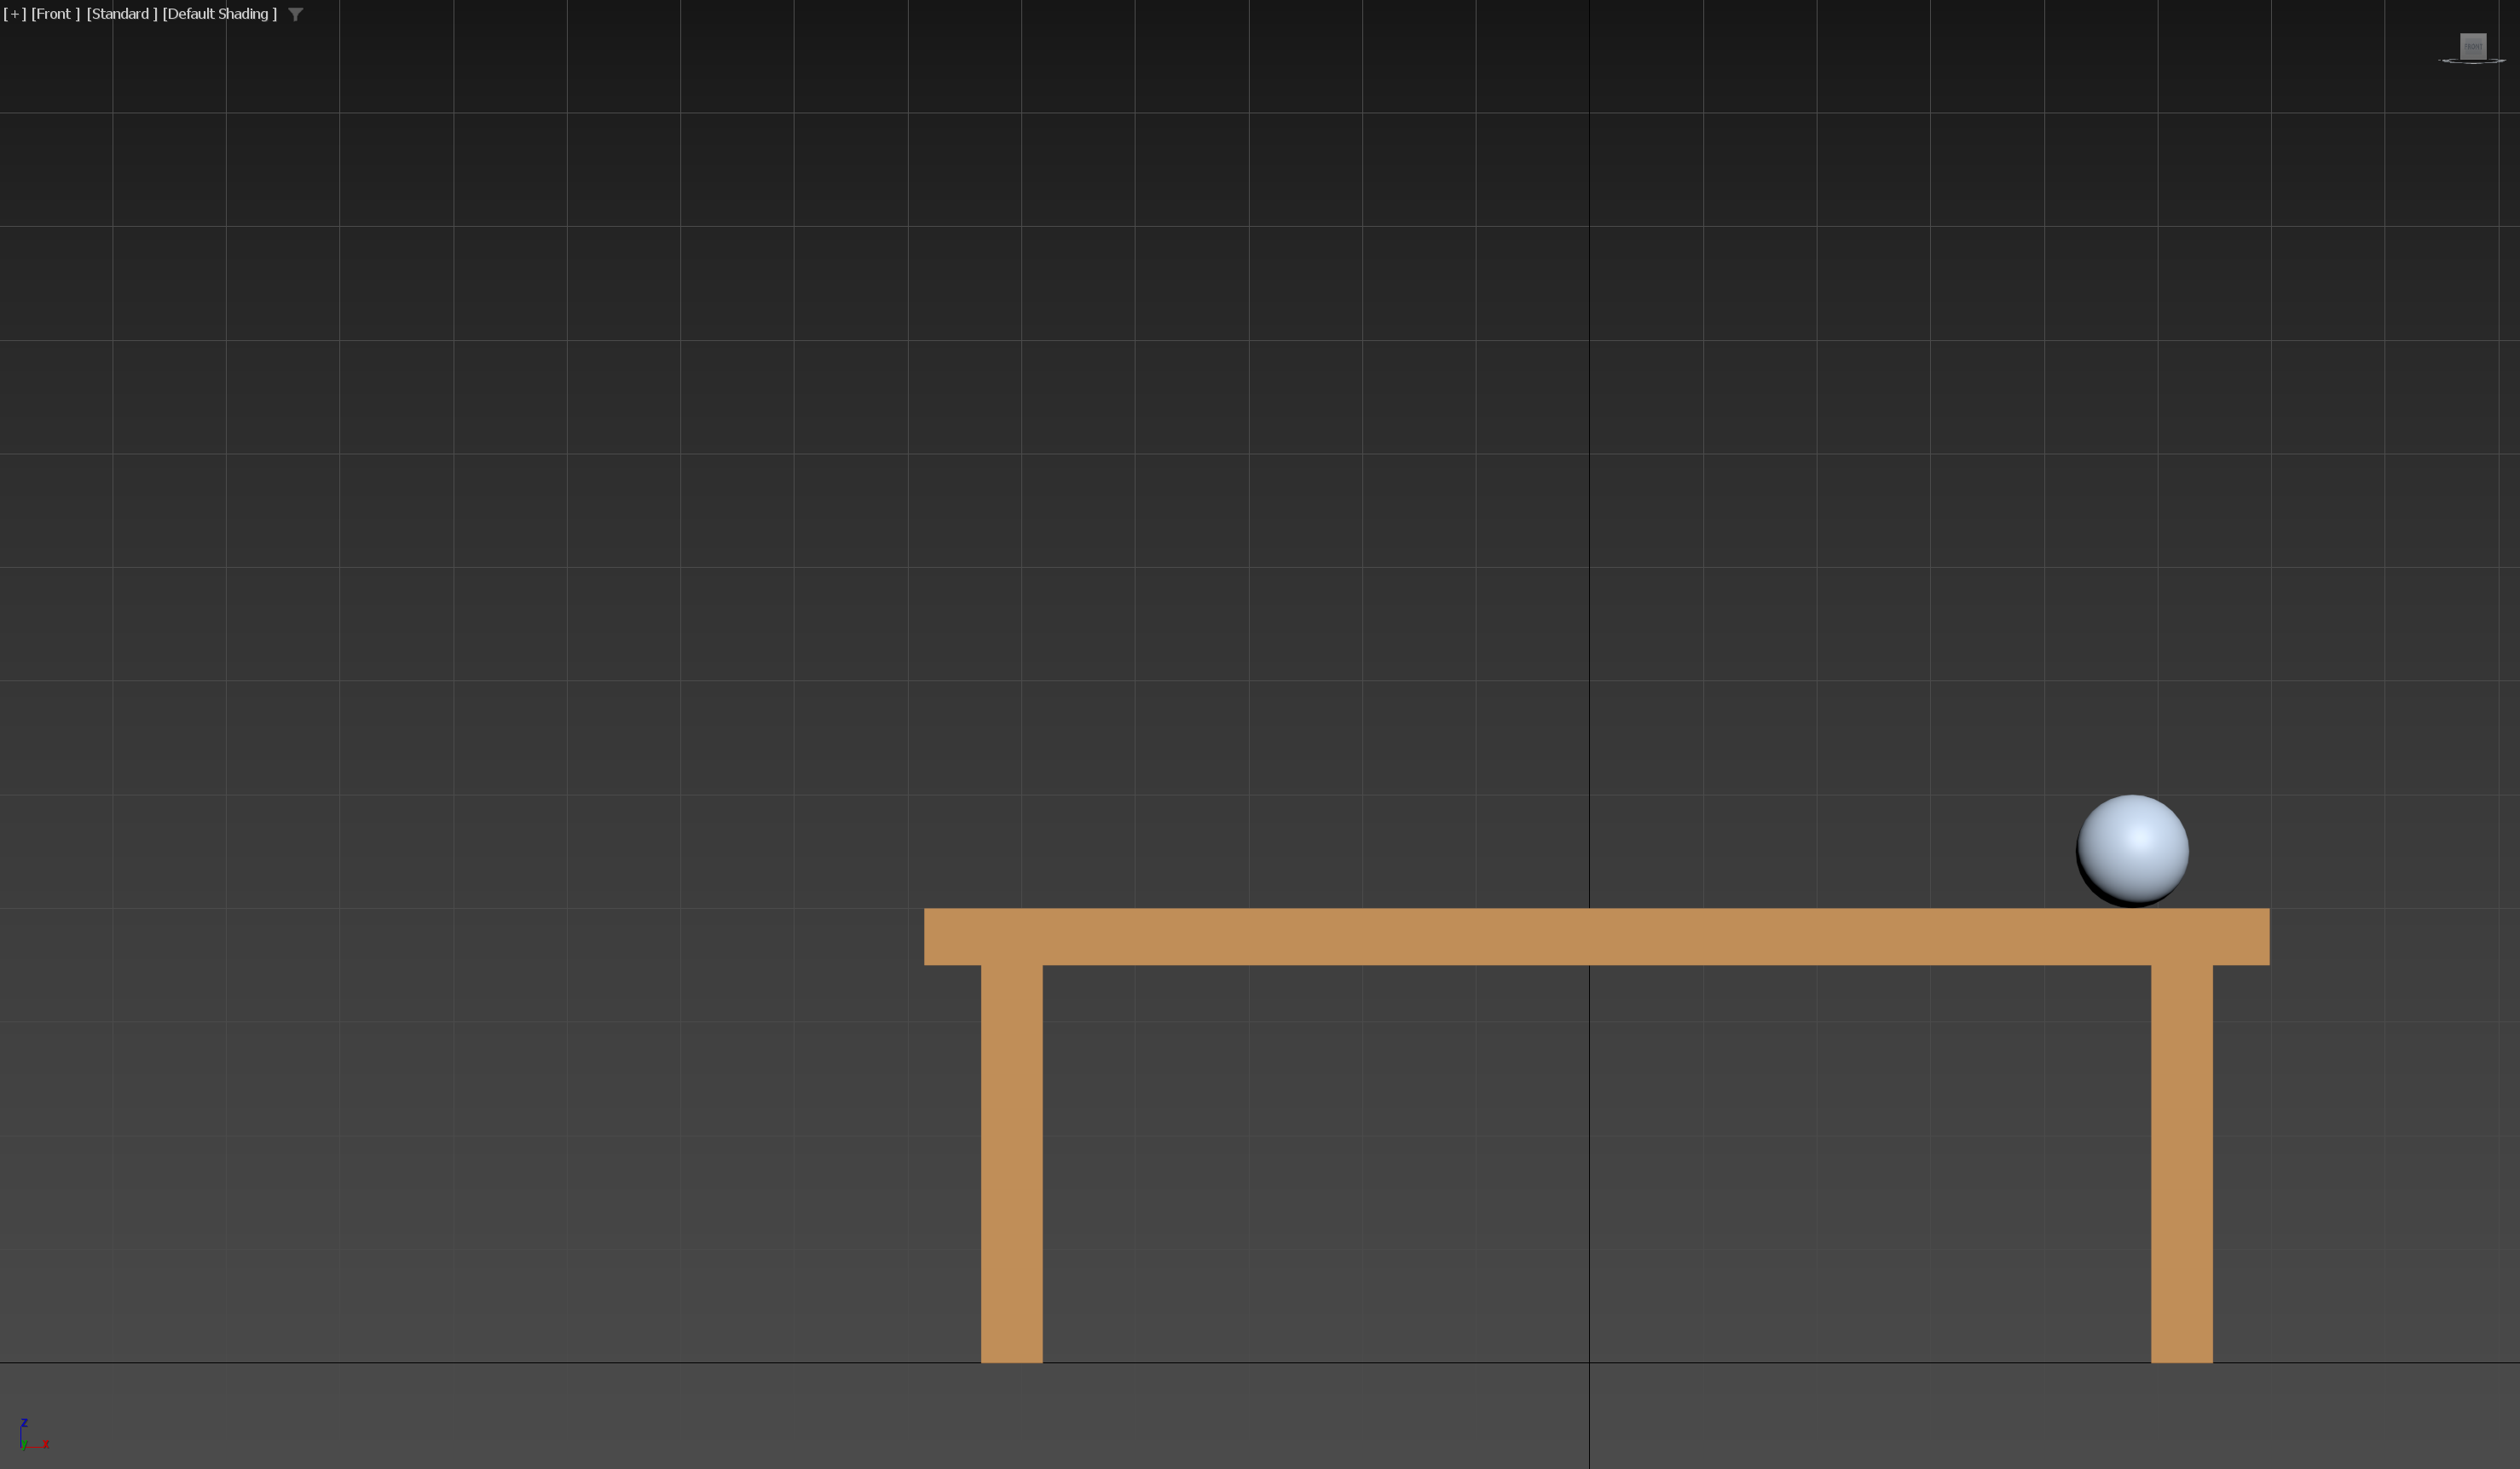
\includegraphics[width=\textwidth]{imagenes/Ejercicio3/keyframes/59.png}
    \caption{Pelota en el instante 59.}
\end{figure}
\begin{figure}[H]
    \centering
    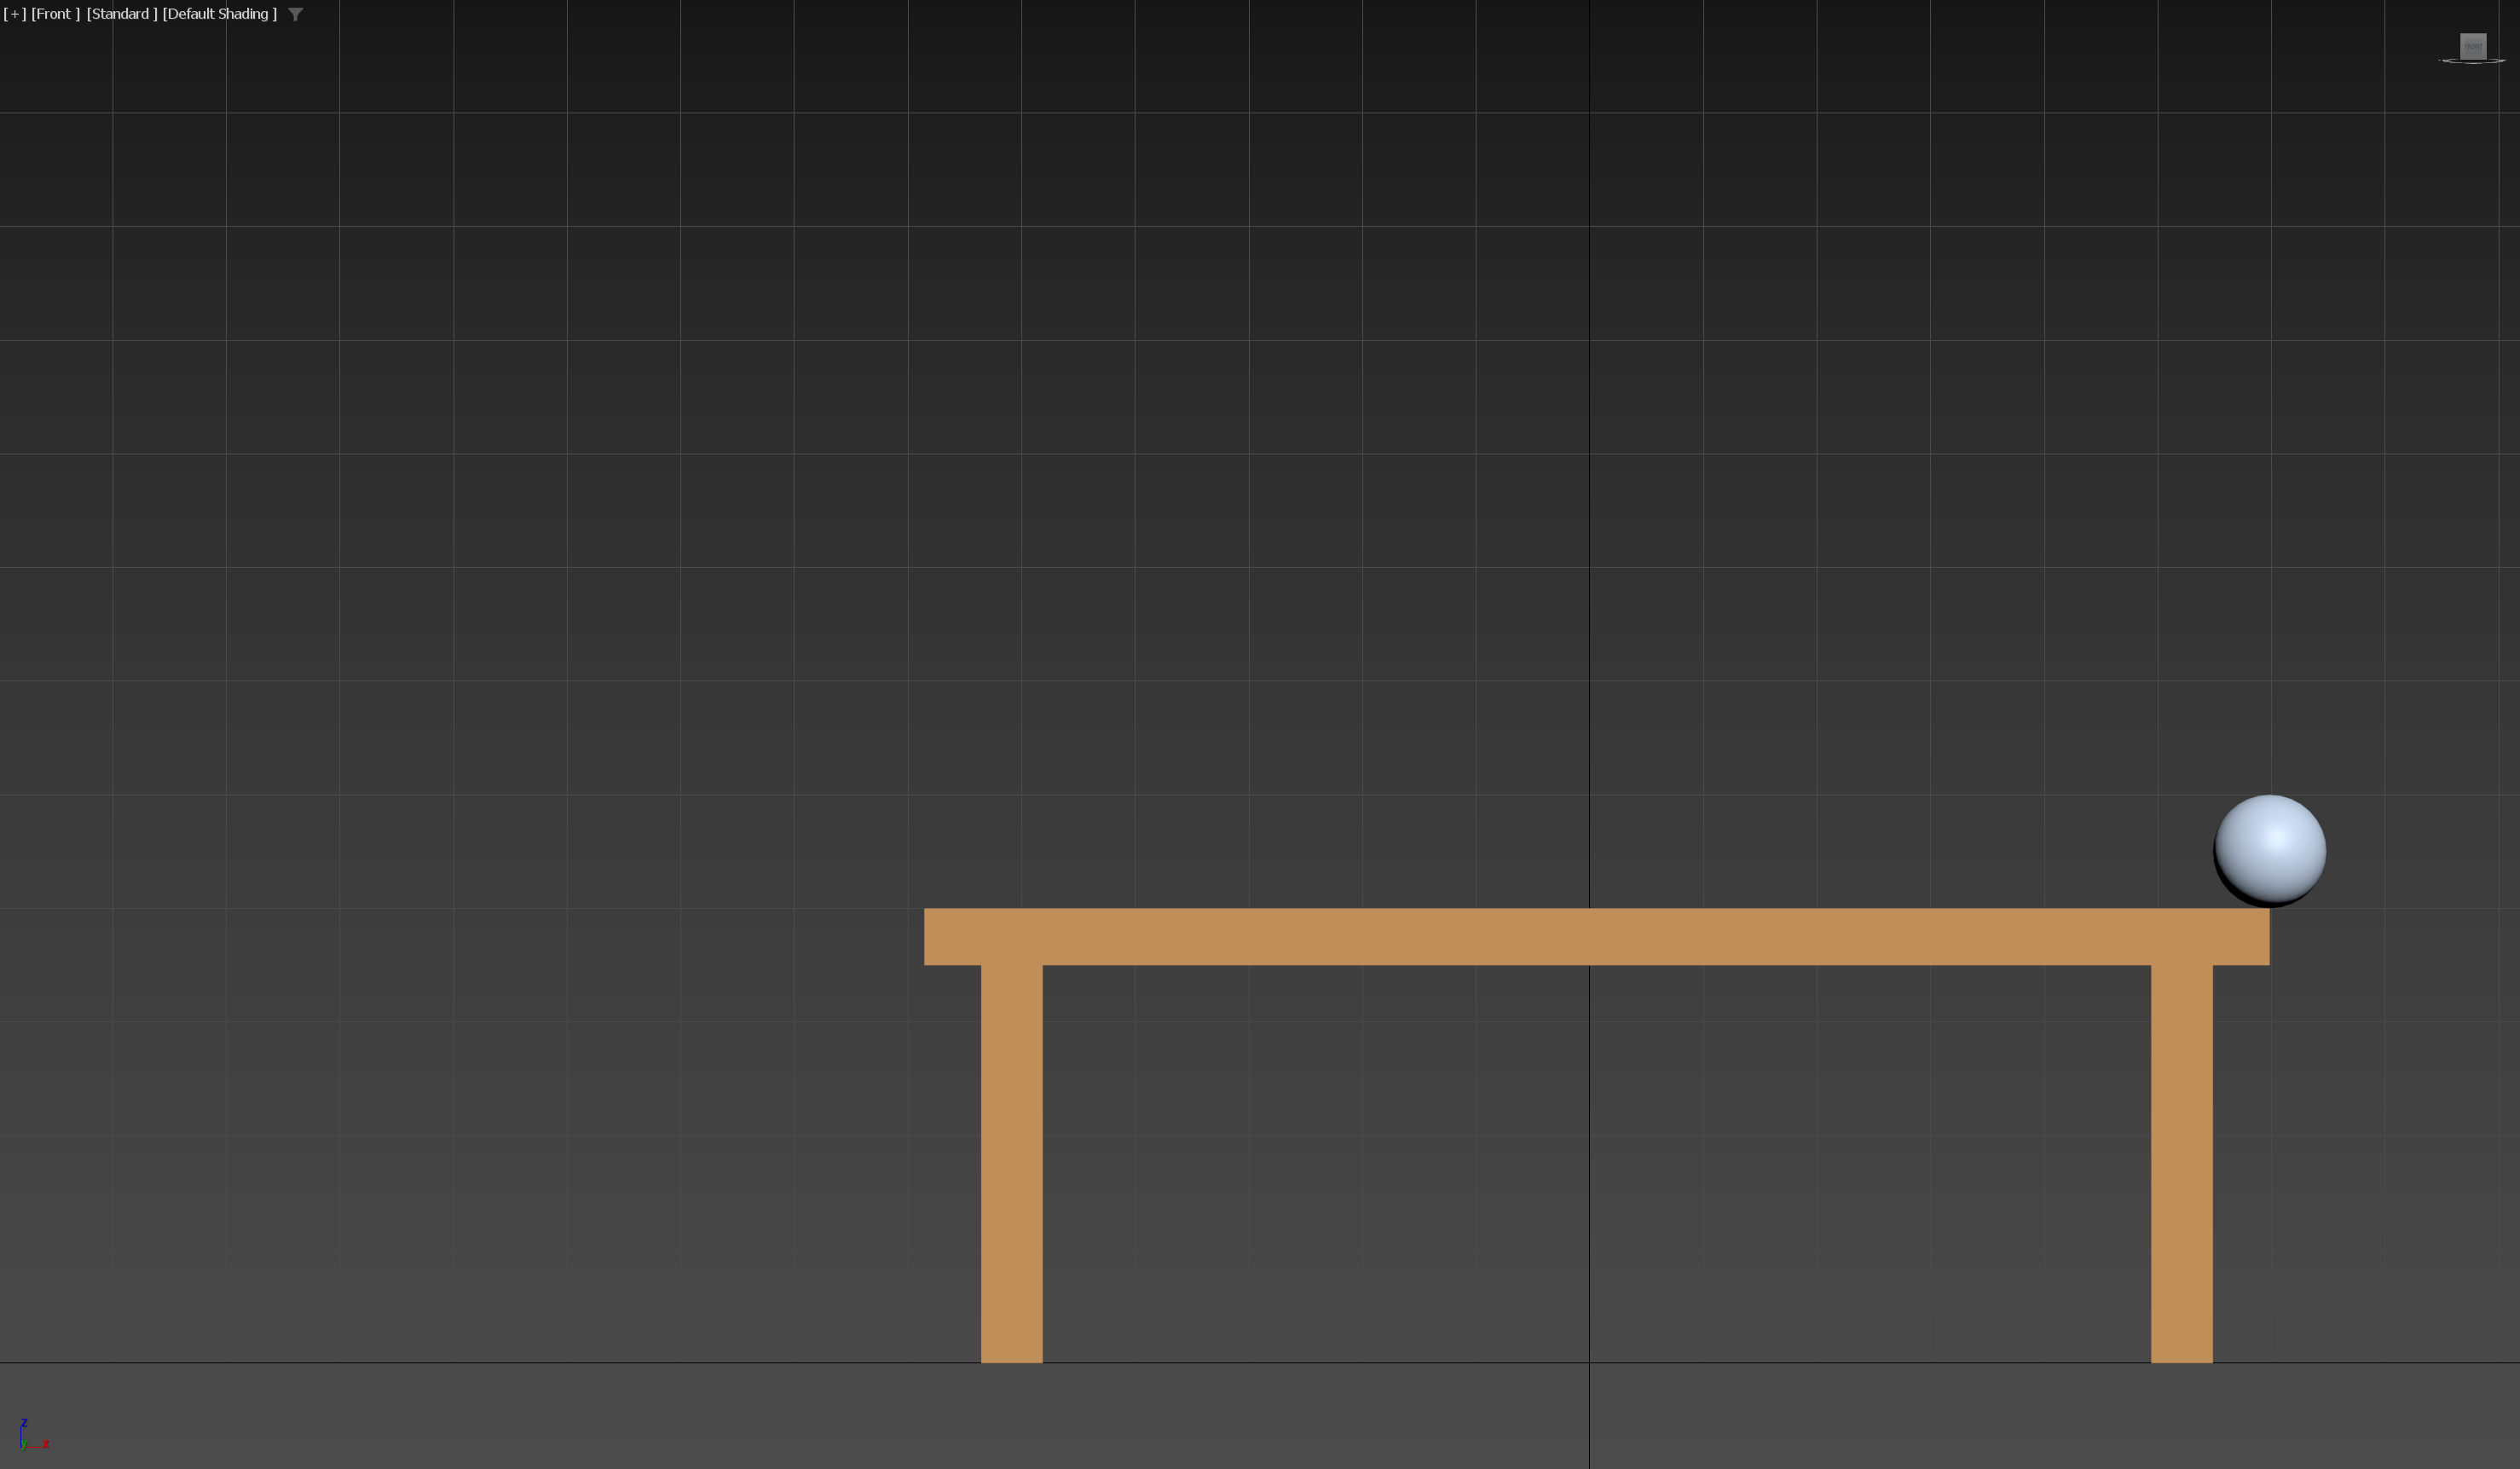
\includegraphics[width=\textwidth]{imagenes/Ejercicio3/keyframes/71.png}
    \caption{Pelota en el instante 71.}
\end{figure}
\begin{figure}[H]
    \centering
    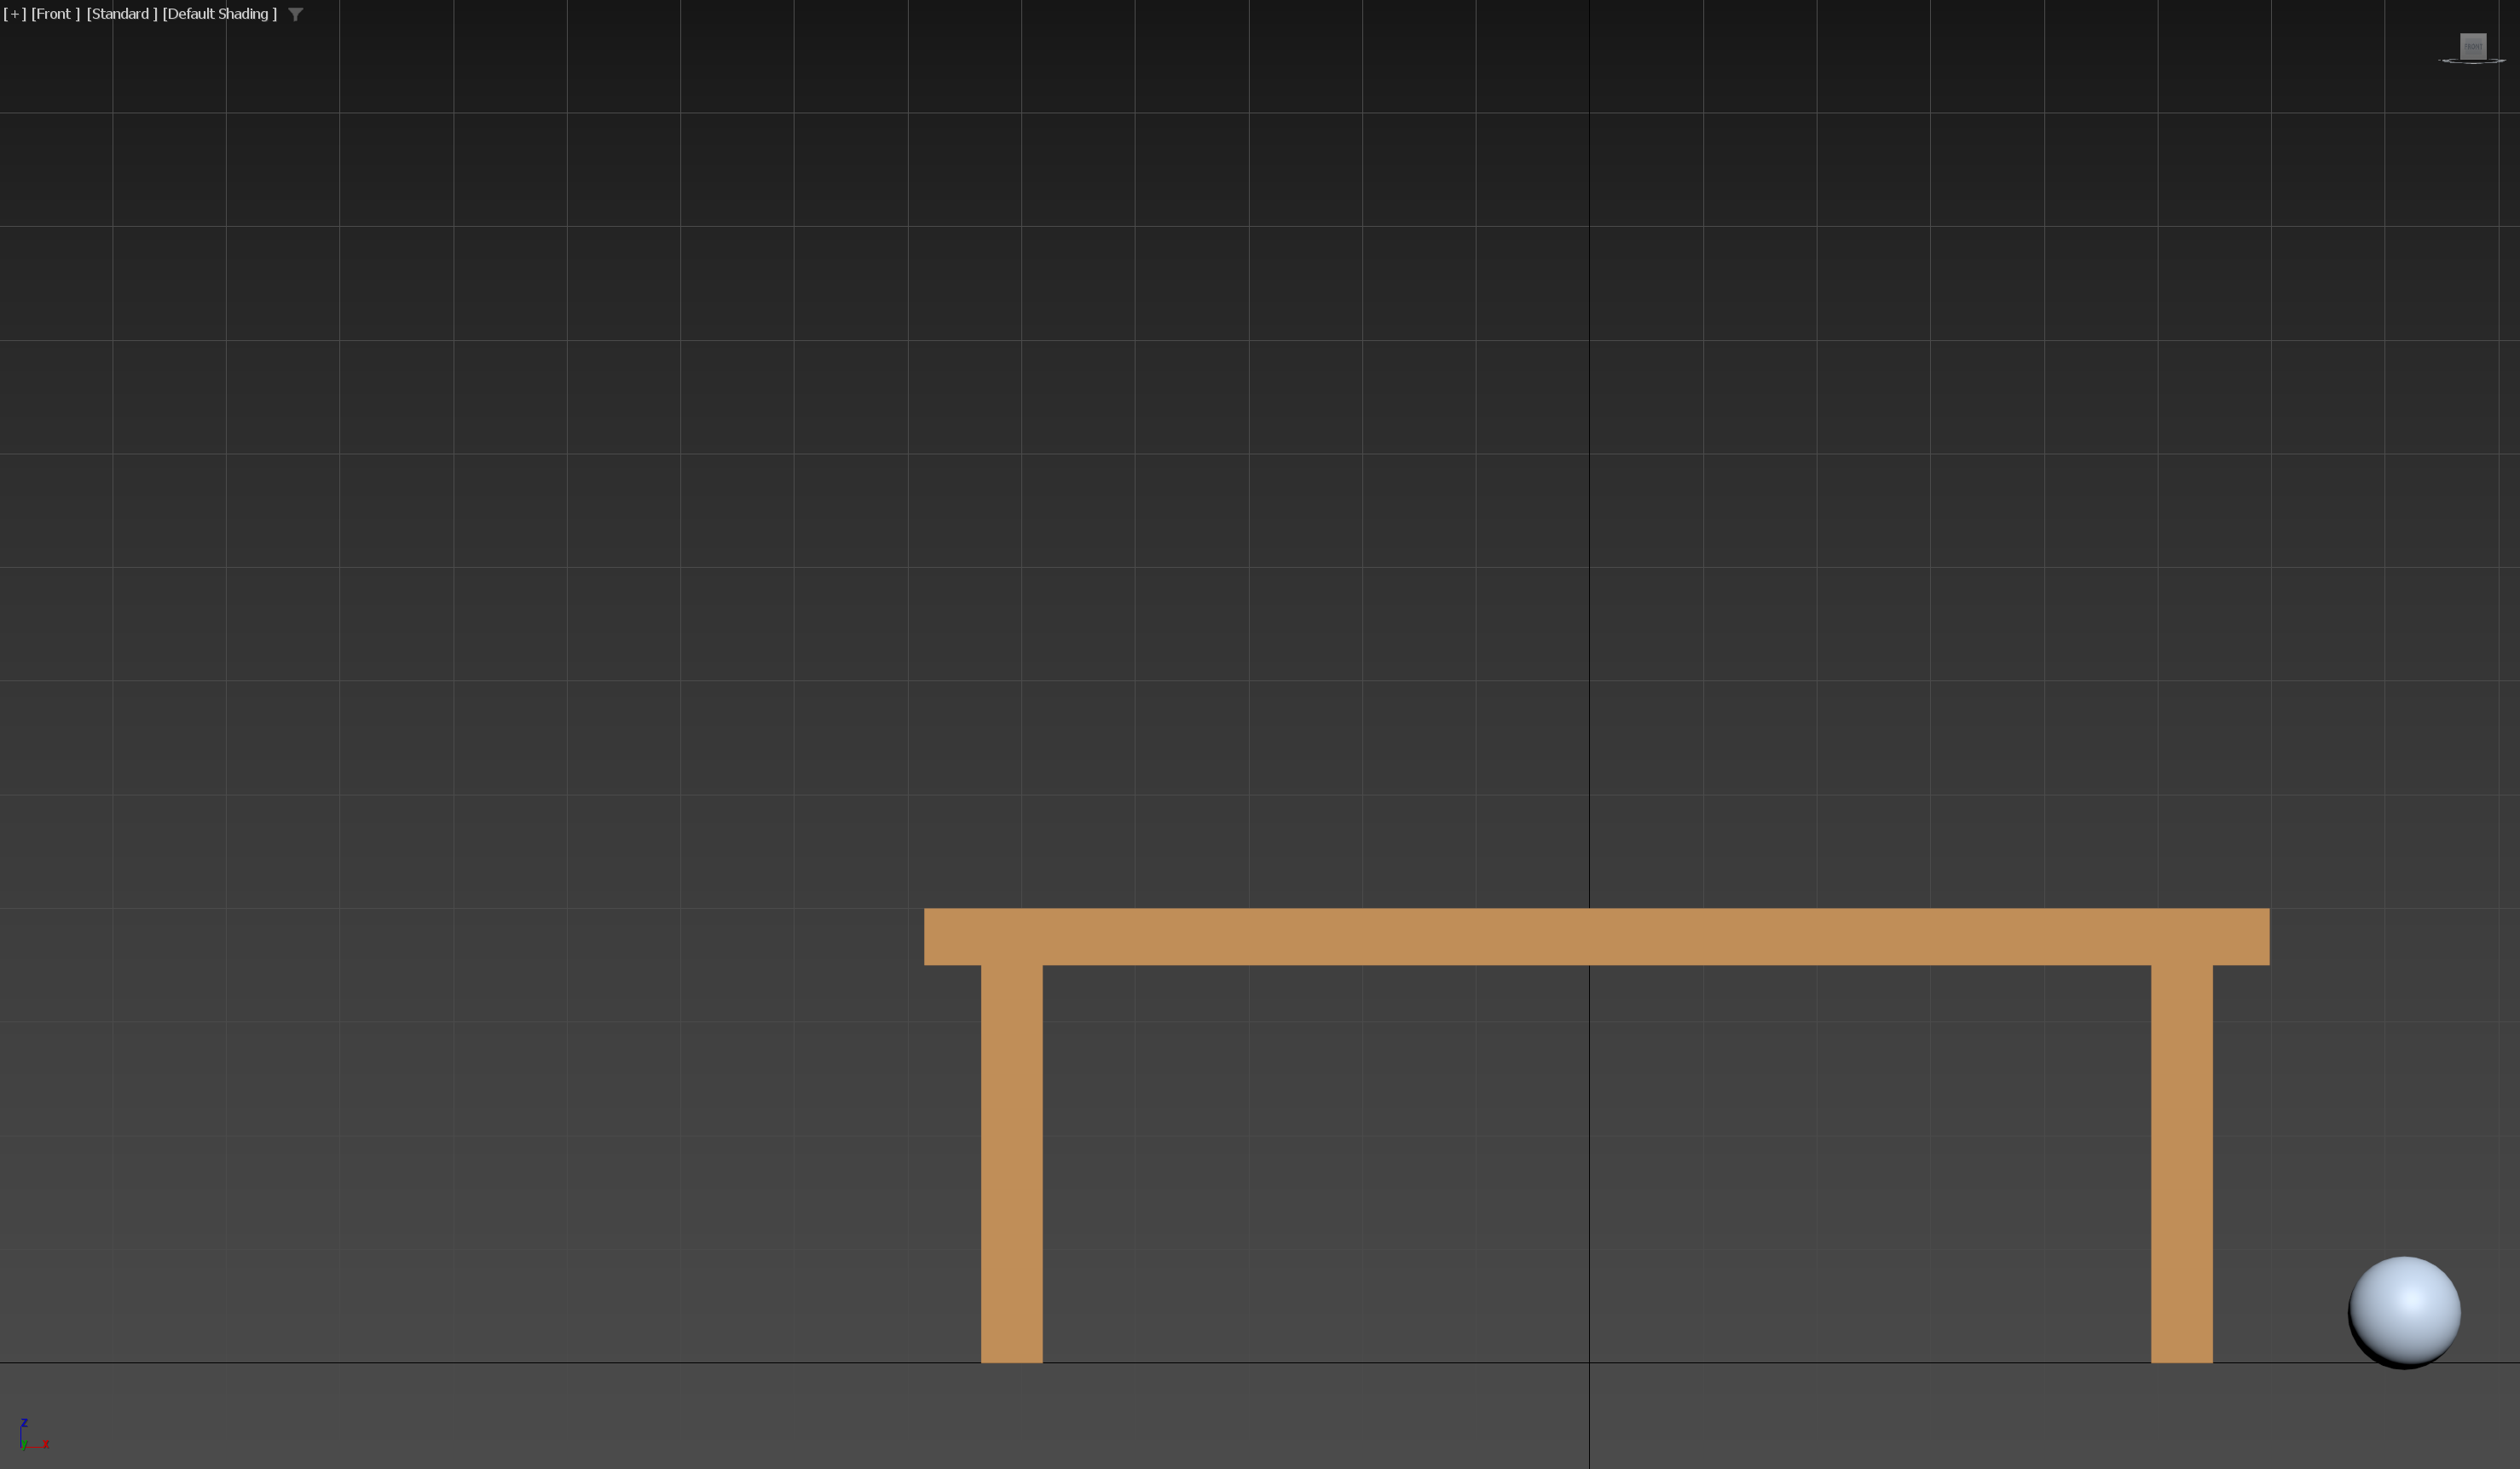
\includegraphics[width=\textwidth]{imagenes/Ejercicio3/keyframes/84.png}
    \caption{Pelota en el instante 84.}
\end{figure}

Y para animar los rebotes y el movimiento de manera realista, se han usado las siguientes curvas en la pelota:

% imagenes separadas de las curvas
\begin{figure}[H]
    \centering
    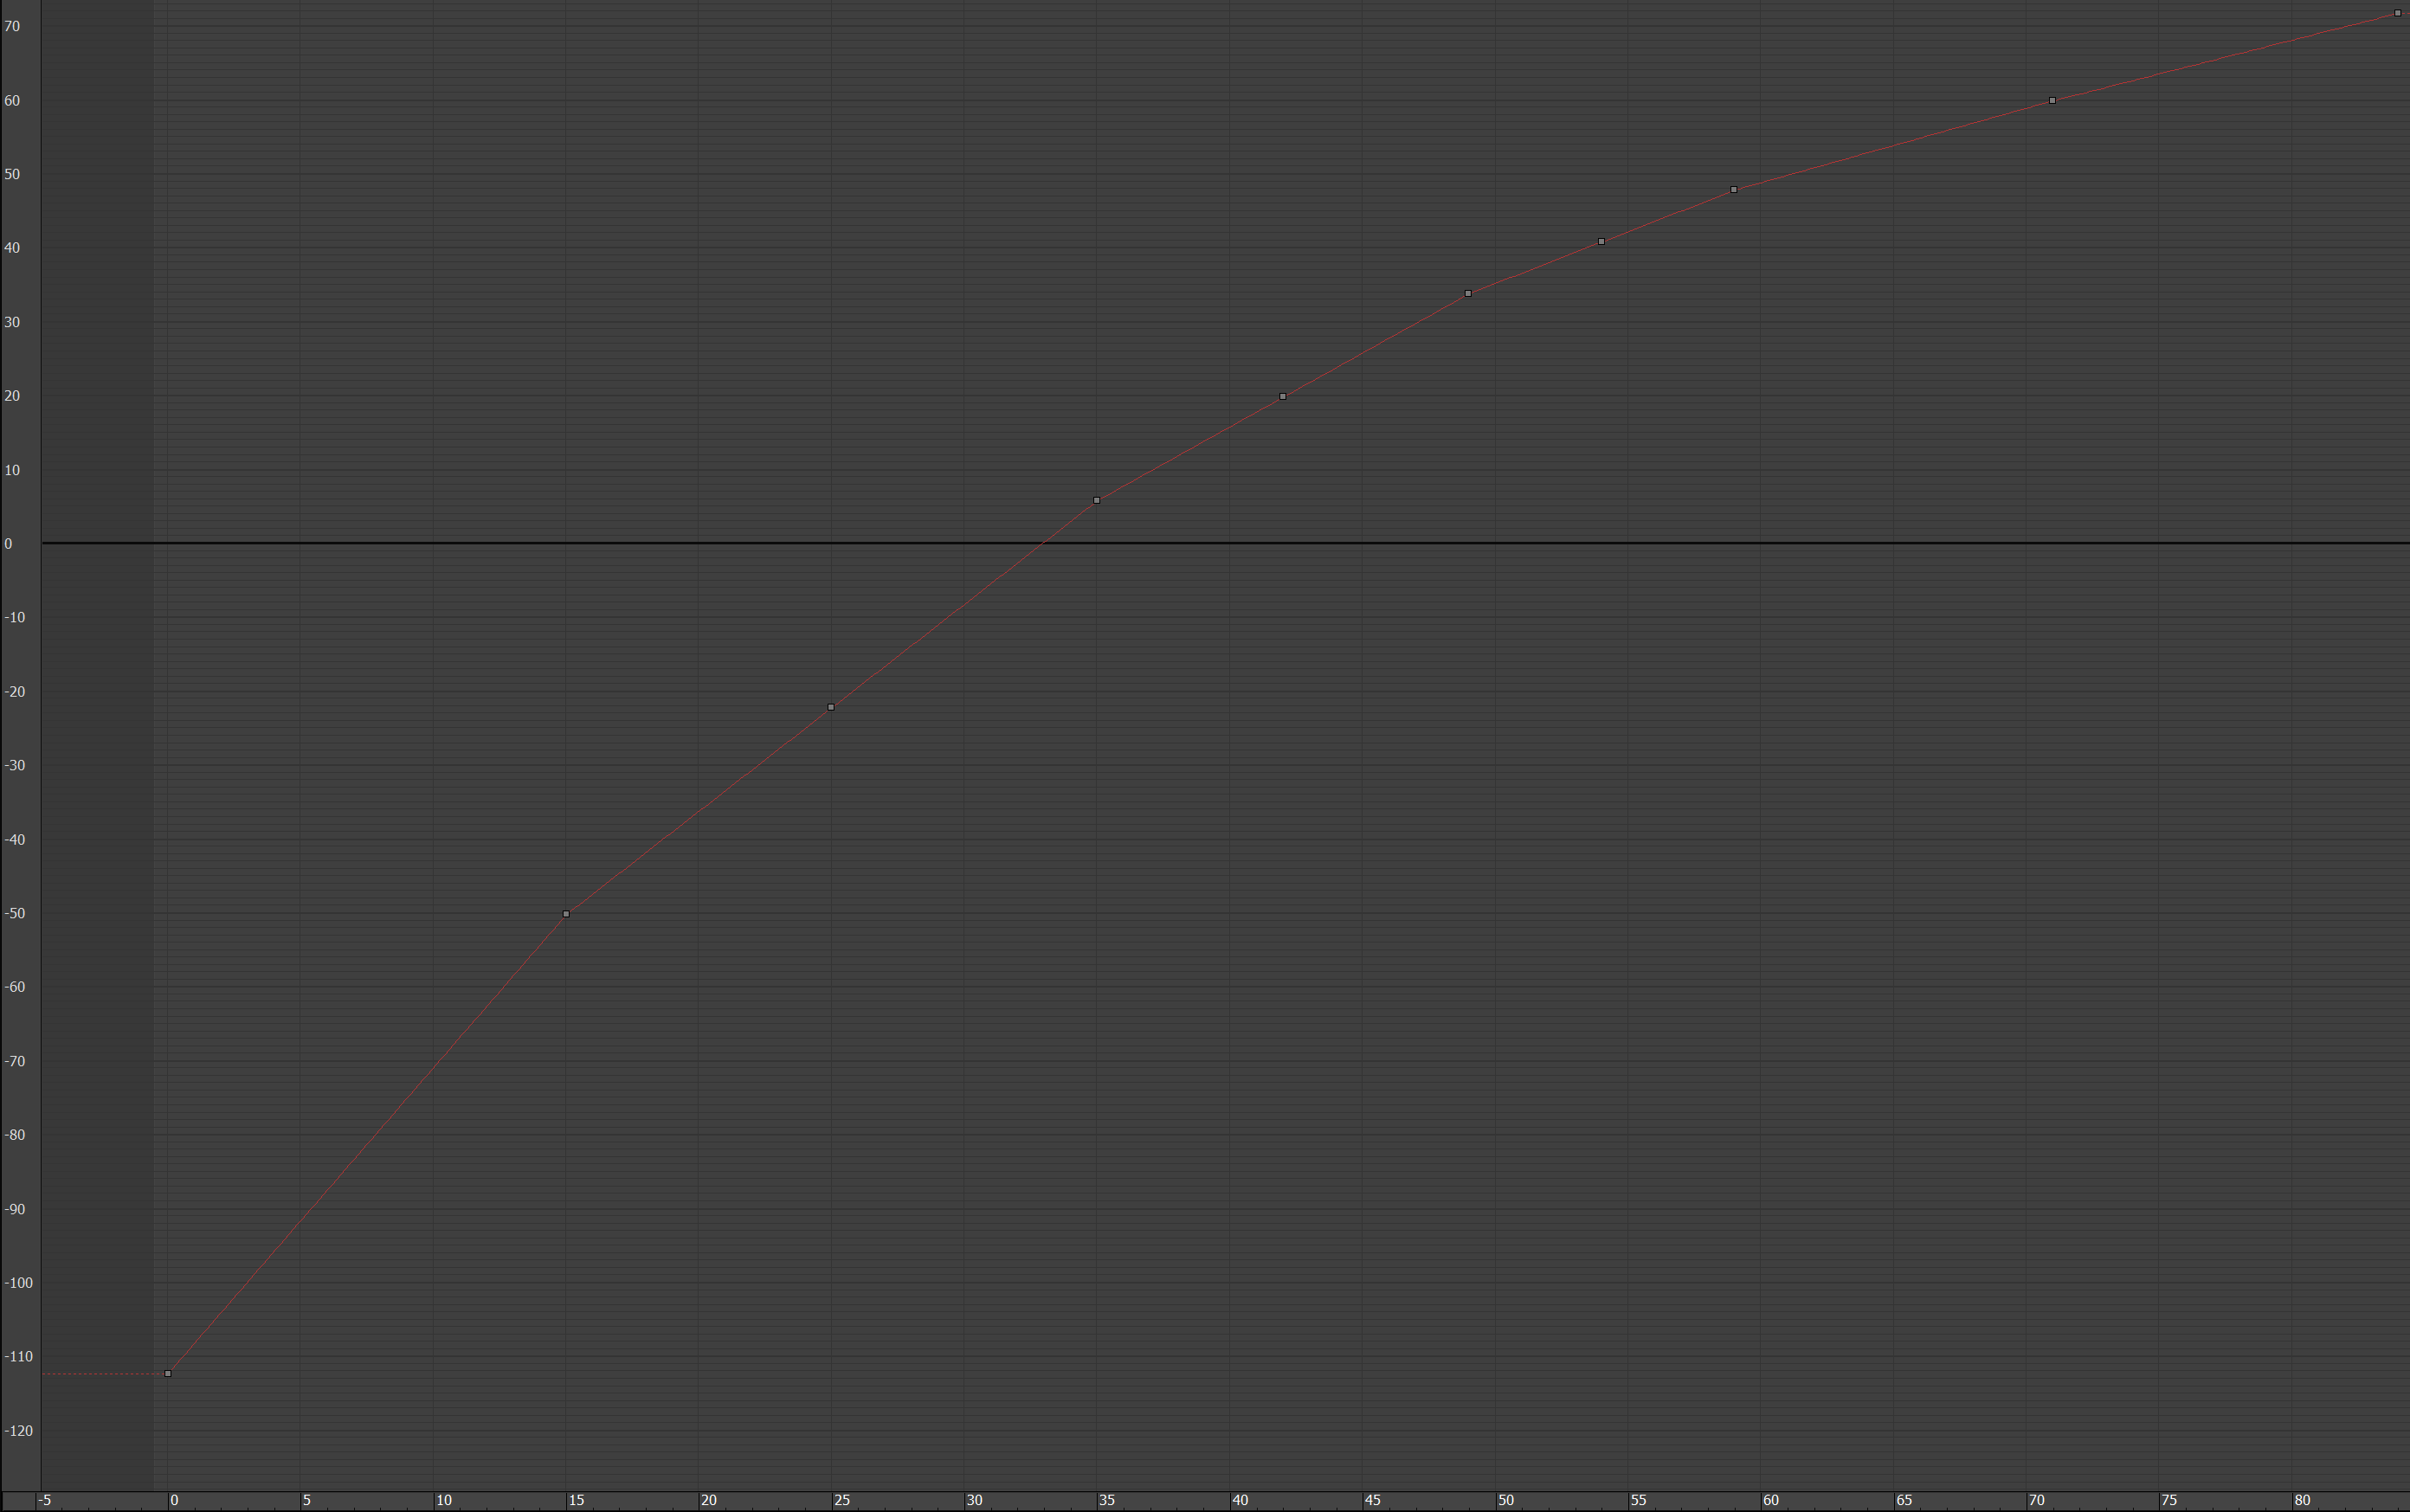
\includegraphics[width=\textwidth]{imagenes/Ejercicio3/curvas/red.png}
    \caption{Posición de la pelota en el eje X.}
\end{figure}

\begin{figure}[H]
    \centering
    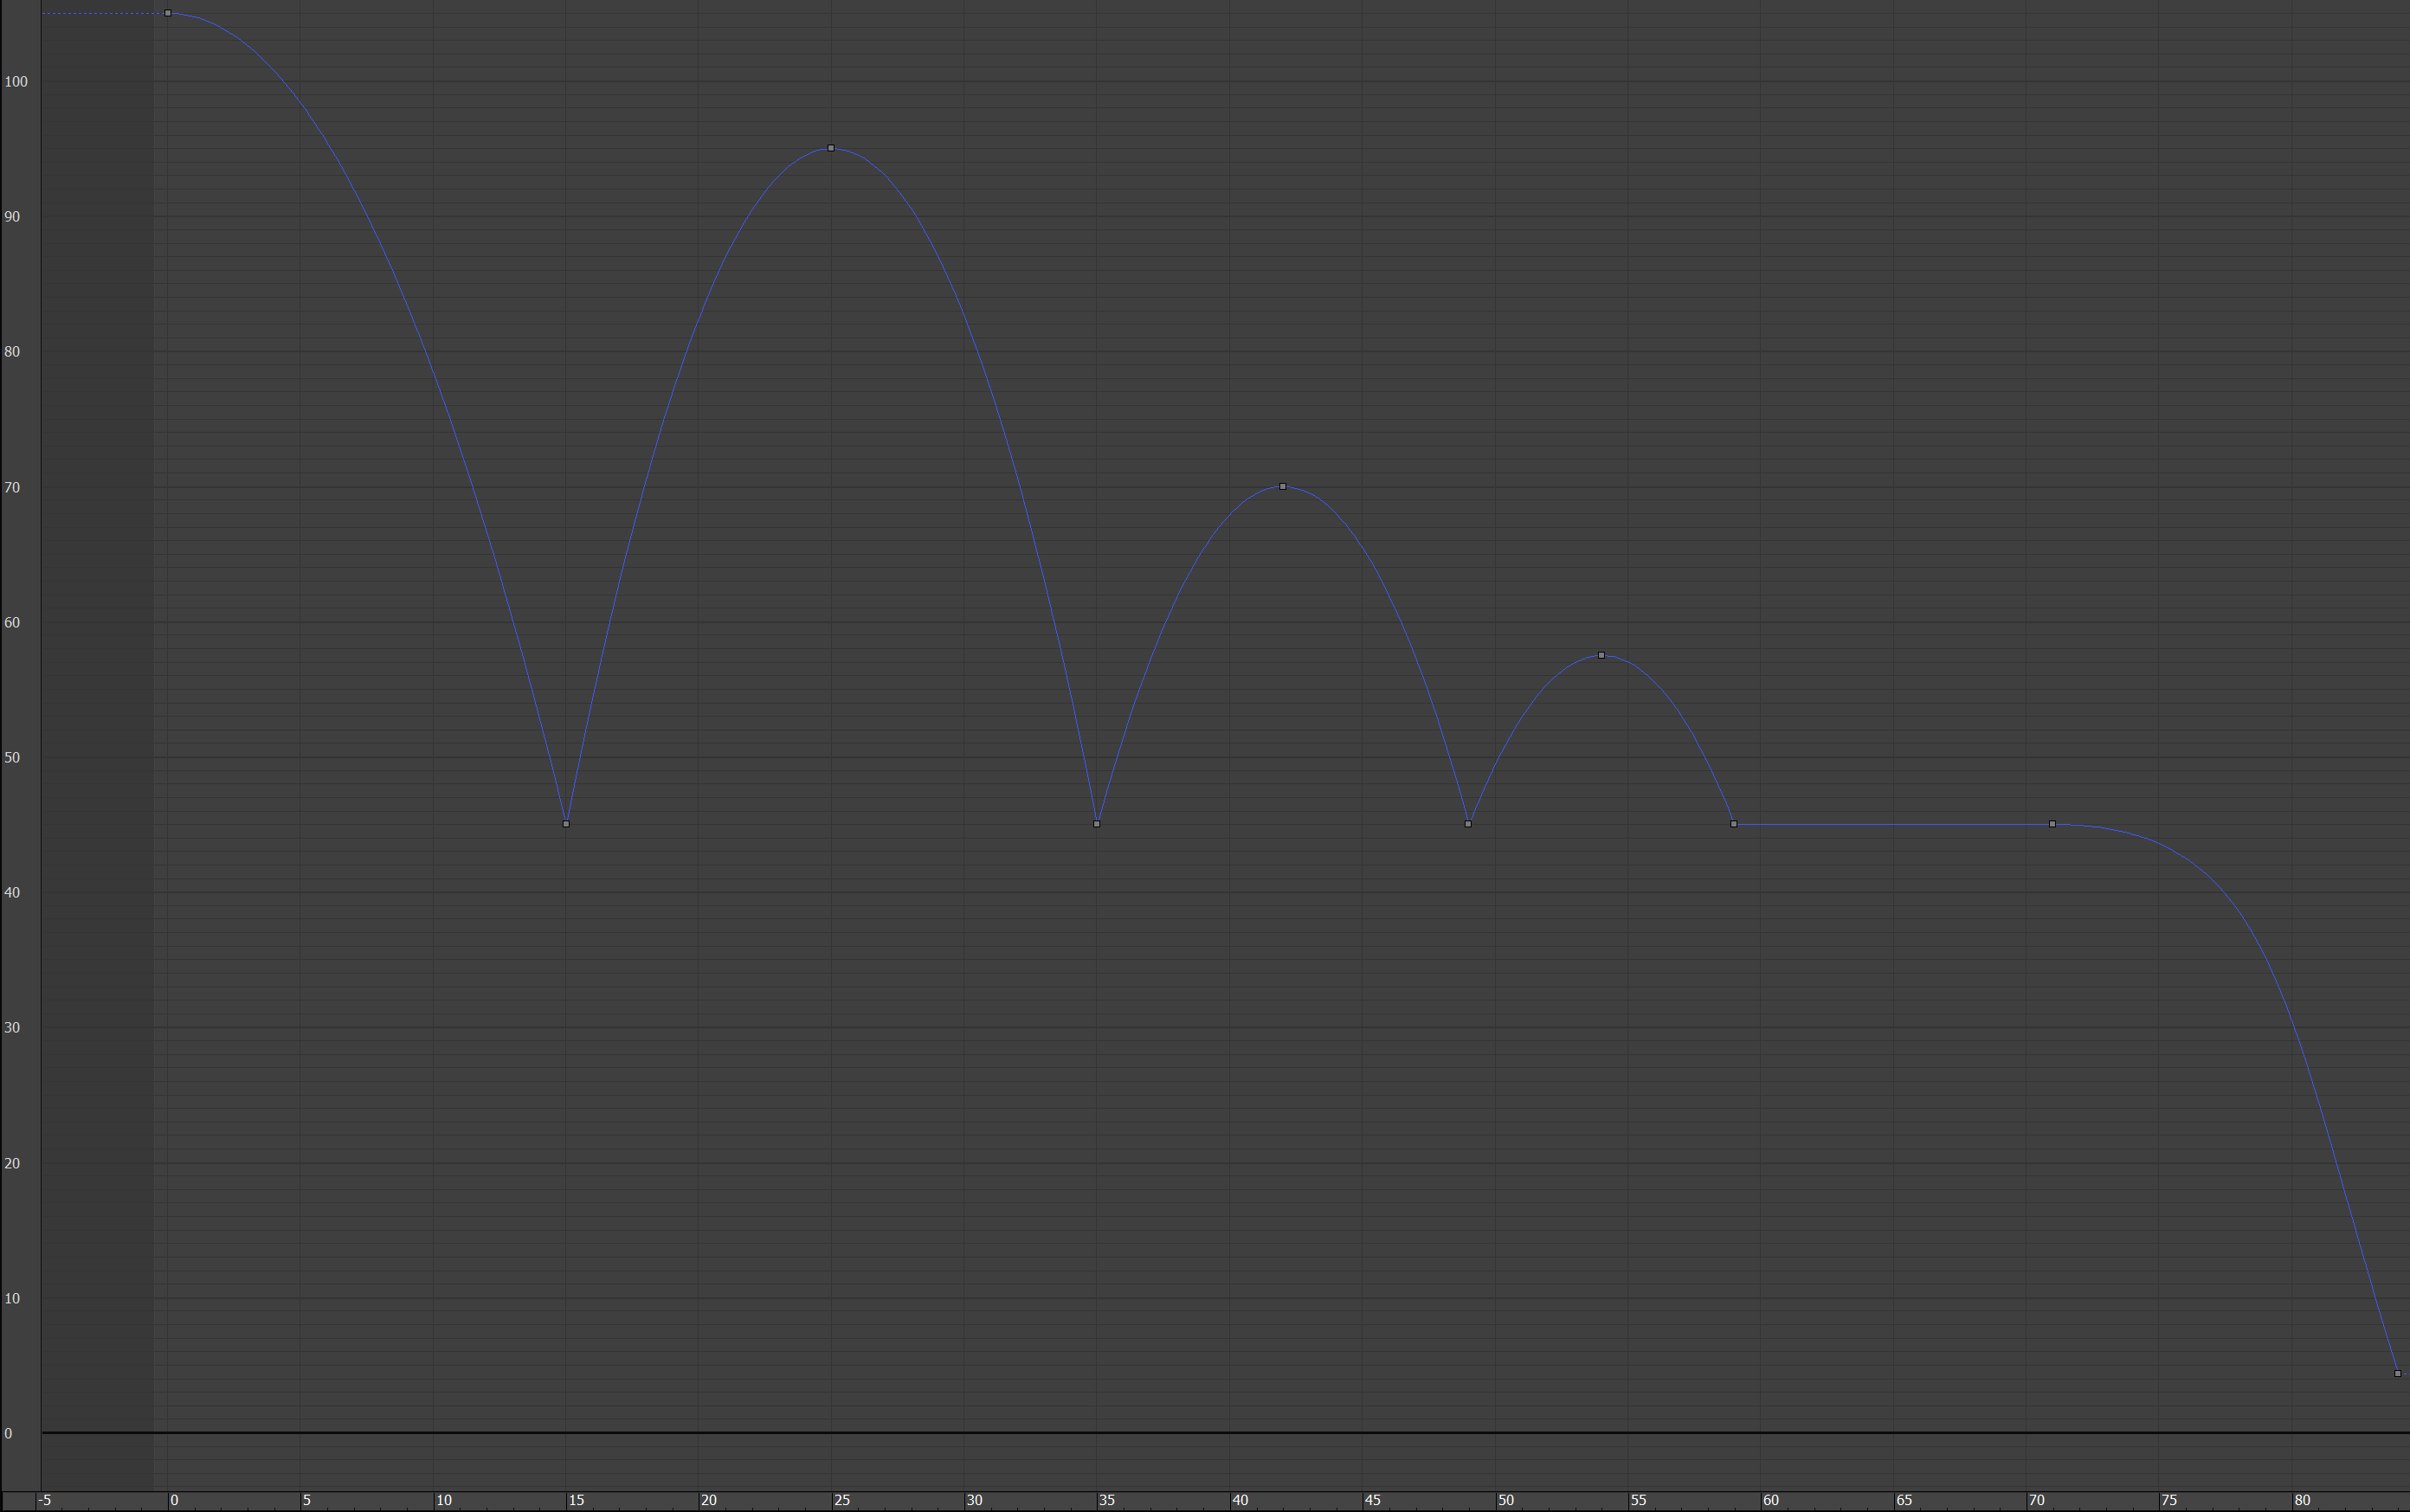
\includegraphics[width=\textwidth]{imagenes/Ejercicio3/curvas/blue.png}
    \caption{Posición de la pelota en el eje Z.}
\end{figure}

La curva de color rojo (Posición en el eje X) sigue una forma lineal para todos los \textit{keyframes}. También se puede observar como el conjunto de todos los \textit{keyframes}, al seguir el factor 2, tiene una forma exponenecial, haciendo que en la animación la pelota vaya recorriendo cada vez menos distancia. 
Esto se podría haber hecho directamente con dos \textit{keyframes} y dicha curva, pero se perdería demasiada precisión. % quizas quitar esto

Mientras que la curva de color azul (Posición en el eje Z) sigue las trayectorias que hace la bola. Para que sean realistas los botes, he utilizado una curva de desaceleración en la subida y otro de aceleración en la bajada, para simular el efecto de la gravedad en la pelota. Cuando cae de la mesa se sigue la misma curva de aceleración.

\section{Ejercicio 4 - Montacargas}

En este ejercicio se pide animar un montacargas que se mueve desde la izquierda hasta la derecha y para burscamente al final aplicando el principio de \textit{Overlap \& Follow Through}. Por tanto, la cadena del montacargas debe ser ``arrastrada'' por la plataforma y cuando esta pare, la cadena debe dar un latigazo en el sentido contrario, para luego detenerse en el sitio final.

%jerarquia de las piezas (reescribir)
La figura del montacargas la he realizado usando como plataforma un cubo achatado y para la cadena he usado como figuras básicas un cilindro y una esfera para la articulación. Usando estas figuras, he anidado las distintas secciones del brazo, haciendo que el hijo sea la pieza de abajo y el padre la de arriba. Así se consigue que el hijo herede las transofrmaciones del padre.

%foto de la jerarquia
\begin{figure}[H]
    \centering
    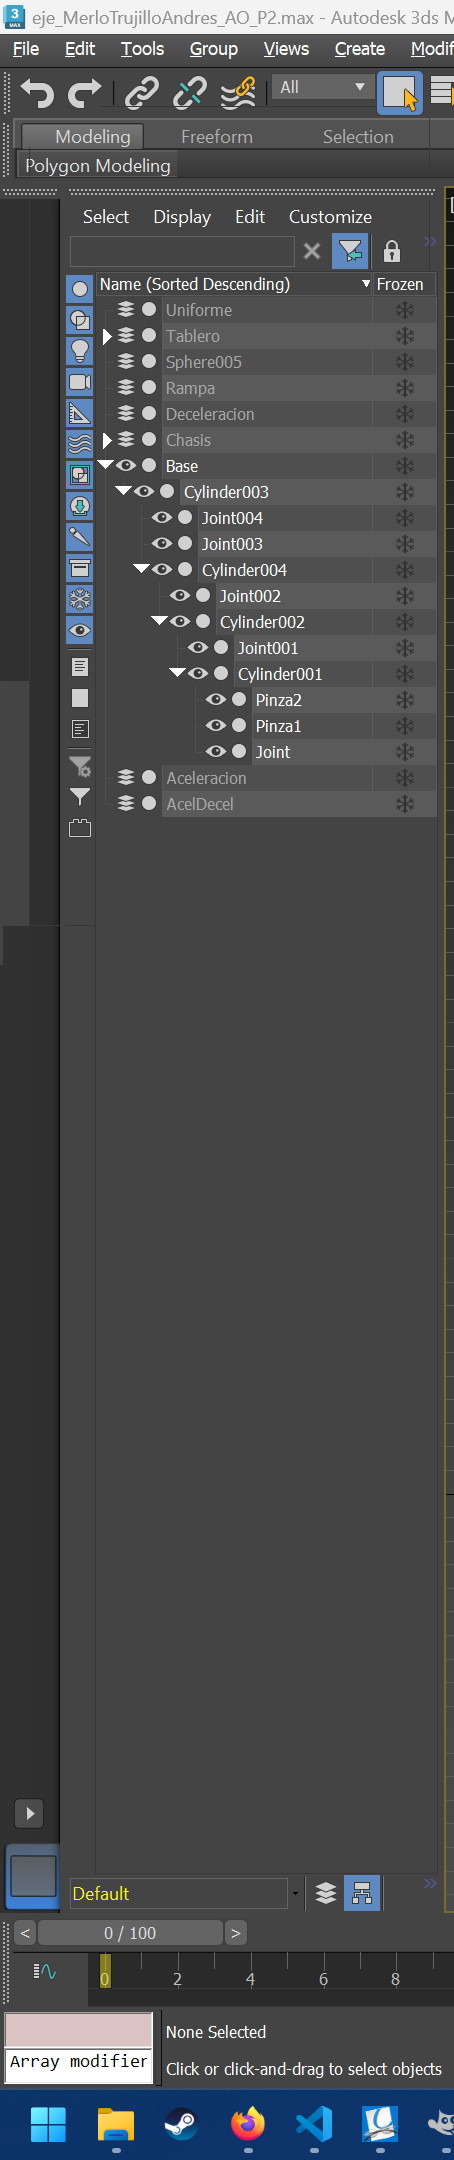
\includegraphics[width=\textwidth]{imagenes/Ejercicio4/jerarquia.png}
    \caption{Jerarquía de las distintas partes del montacargas.}
\end{figure}

En cuanto a la animacion, ha sido necesario utilizar 2 \textit{keyframes} para la plataforma y 7 \textit{keyframes} para cada una de las partes del brazo, pero que realizan exactamente lo mismo. 

\textit{Keframes} de la plataforma:


\begin{enumerate}
    \item Instante 0: Posición inicial, a la izquierda del todo.
    \item Instante 30: Posición final, a la derecha del todo.
\end{enumerate}

\textit{Keframes} generales del brazo:

\begin{enumerate}
    \item Instante 0: Se encuentra el segmento en reposo; es decir, en vertical.
    \item Instante 18: Se encuentra cada segmento del brazo rotado al máximo, siendo arrastrado por la plataforma en movimiento.
    \item Instante 30: Exactamente igual que antes, pero en este caso la plataforma ya ha parado.
    % arreglar parada en seco con otras palabras
    \item Instante 47: Cada segmento del brazo ahora se encuentra rotado al lado contrario, fruto de la parada en seco de la plataforma, haciendo que de un latigazo.
    \item Instante 64: Cada segmente vuelve a estar rotado hacia el otro lado, pero esta vez con una rotación algo menor que la primera vez, simulando las distintas fuerzas que actuan.
    \item Instante 80: Los segmentos vuelven a estar rotados al lado contrario, pero con una cantidad de rotación mucho menor, casi vertical.
    \item Instante 96: Los segementos se encuentran de nuevo verticales, como en el instante 0.
\end{enumerate}
%keyframes

A modo visual, los \textit{keyframes} son los siguientes:

\begin{figure}[H]
    \centering
    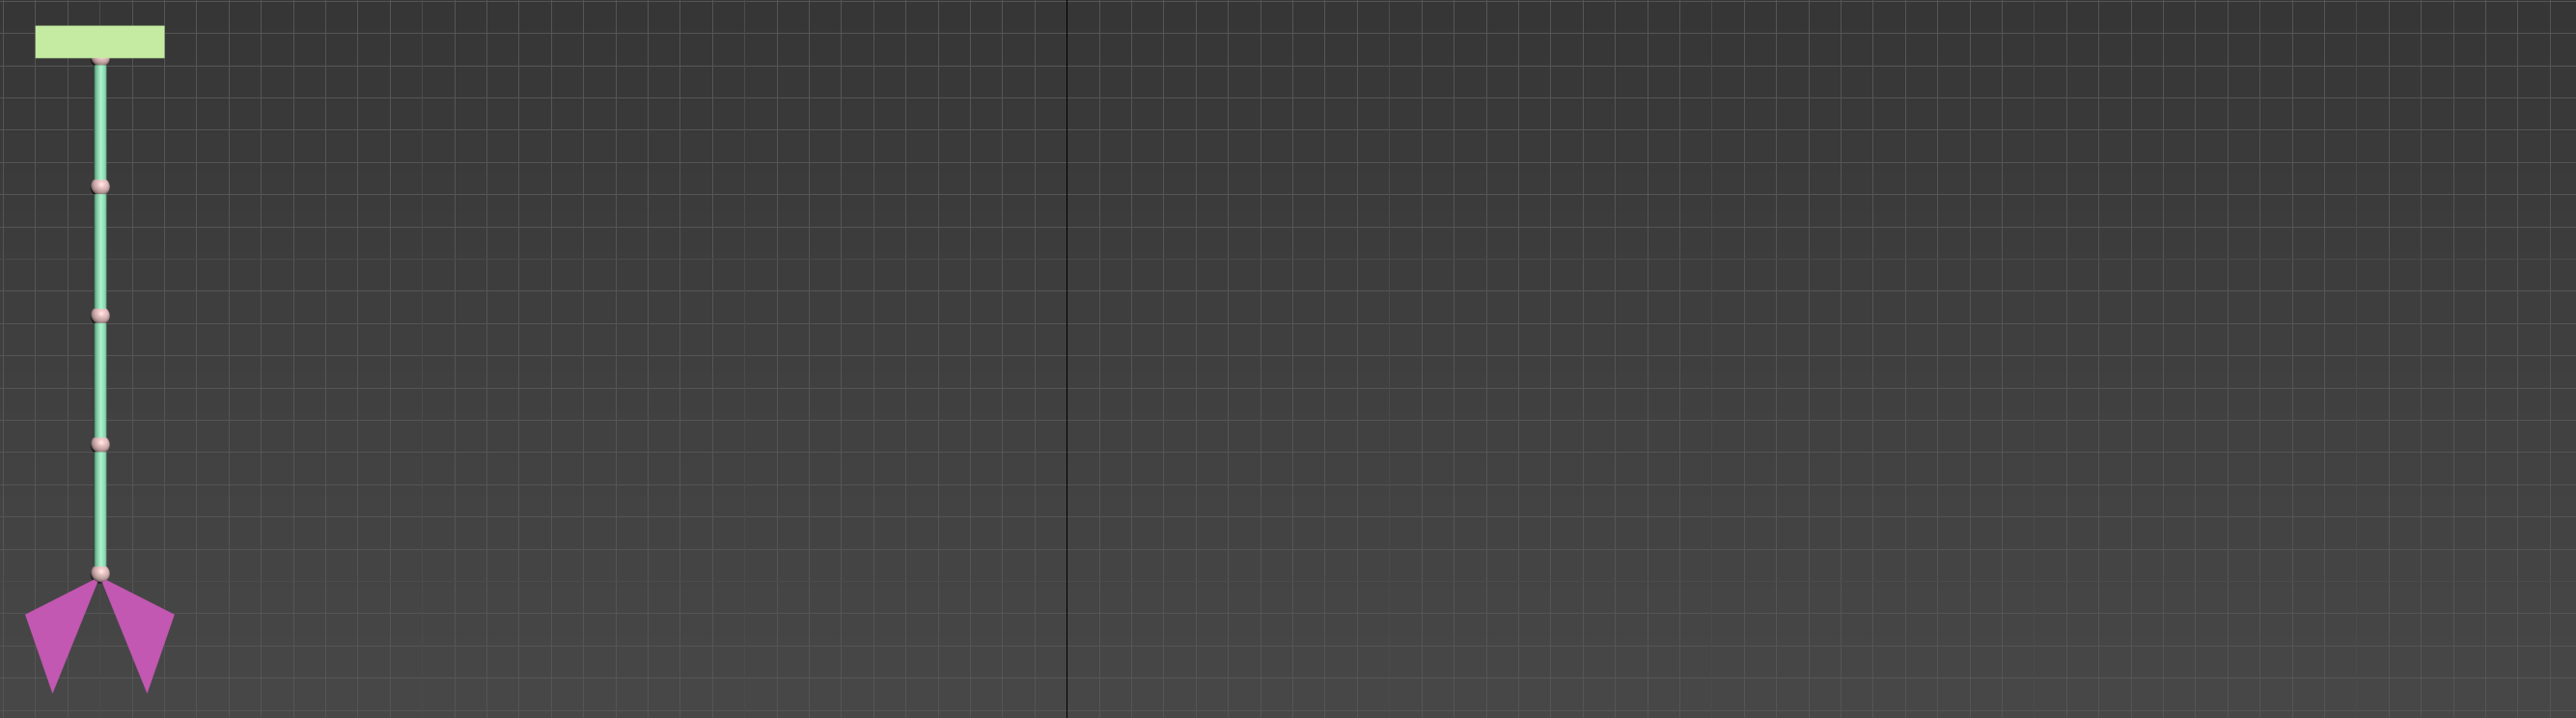
\includegraphics[width=\textwidth]{imagenes/Ejercicio4/keyframes/0.png}
    \caption{Rotación de los segmentos del brazo en el instante 0. También posición inicial de la plataforma.}
\end{figure}

\begin{figure}[H]
    \centering
    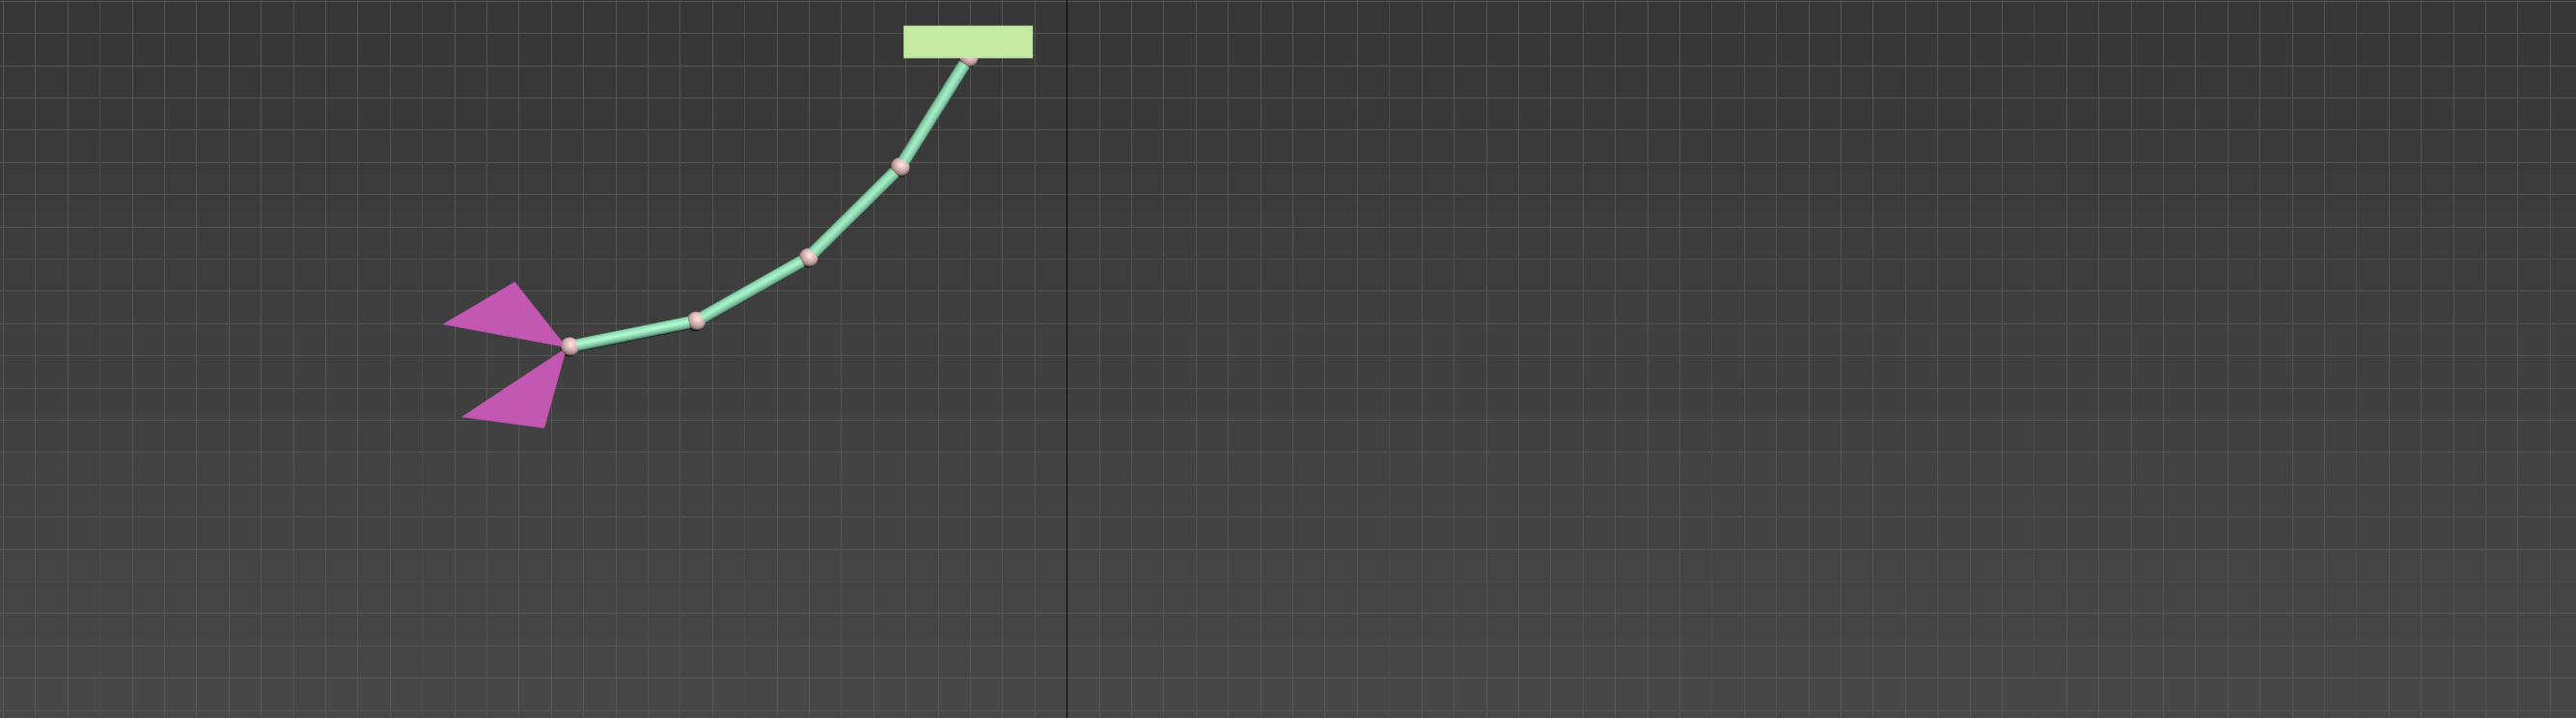
\includegraphics[width=\textwidth]{imagenes/Ejercicio4/keyframes/18.png}
    \caption{Rotación de los segmentos del brazo en el instante 18.}
\end{figure}

\begin{figure}[H]
    \centering
    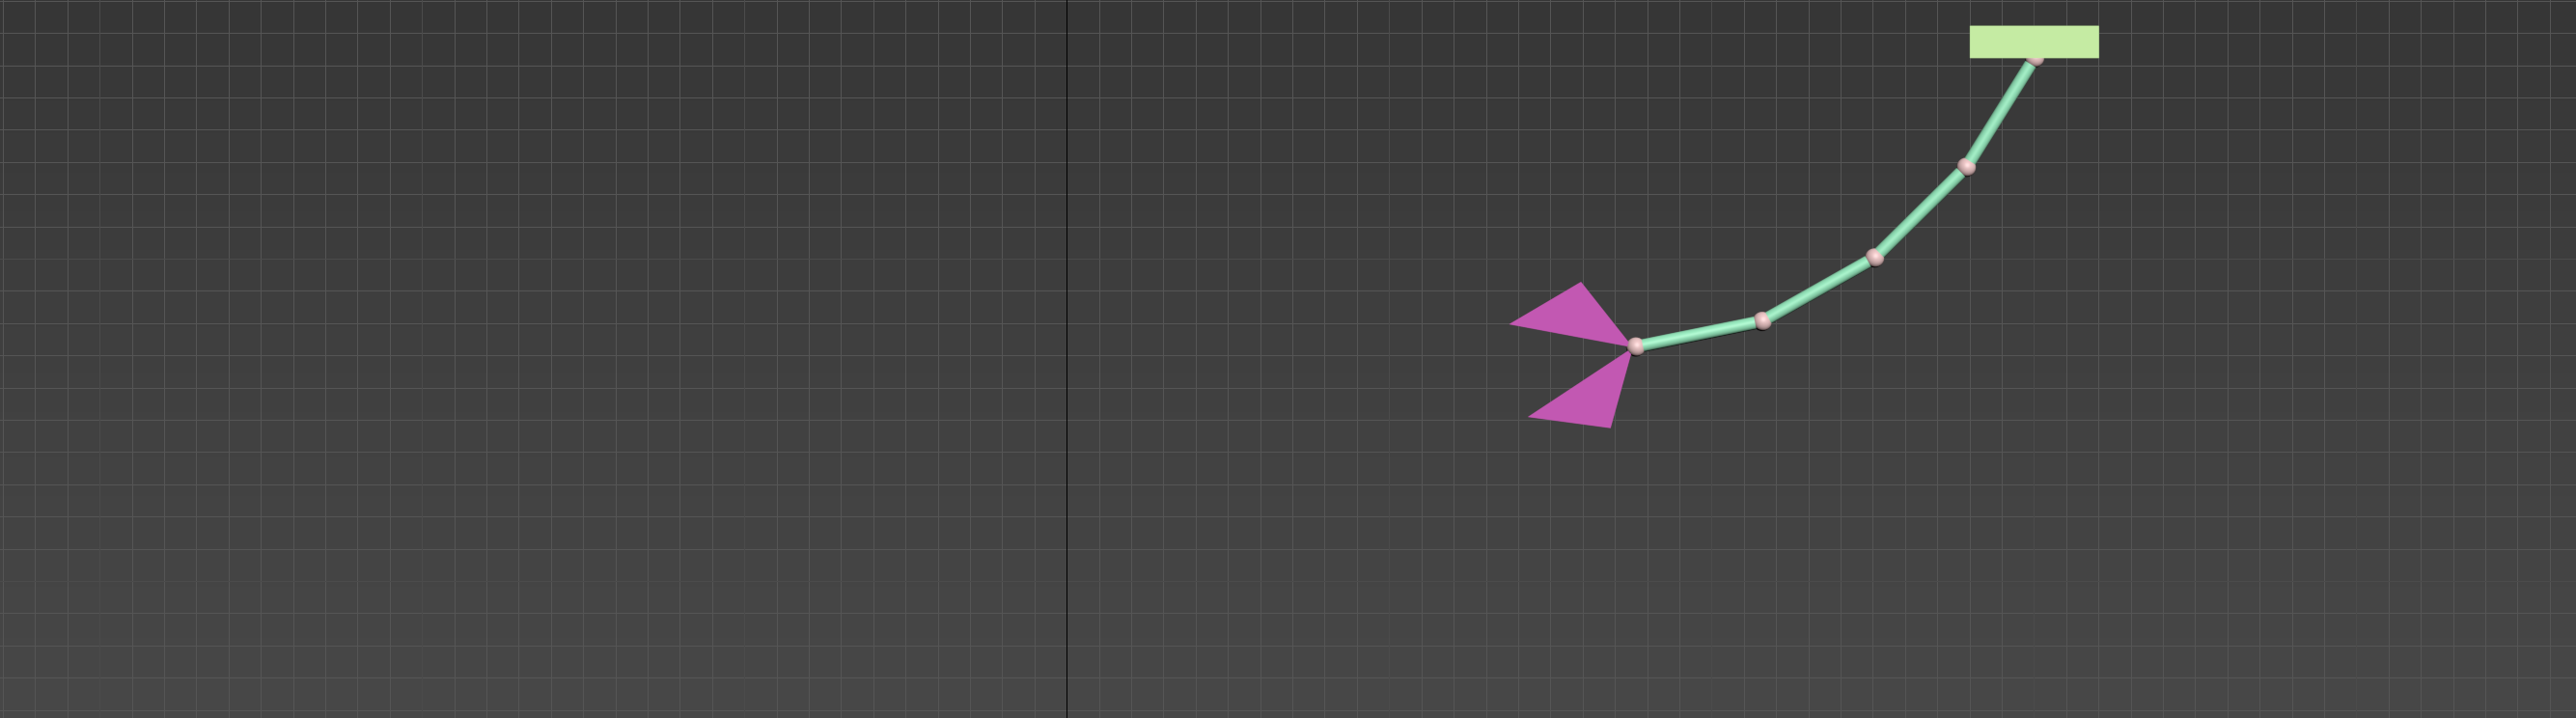
\includegraphics[width=\textwidth]{imagenes/Ejercicio4/keyframes/30.png}
    \caption{Rotación de los segmentos del brazo en el instante 30. Tambien posicion final de la plataforma.}
\end{figure}

\begin{figure}[H]
    \centering
    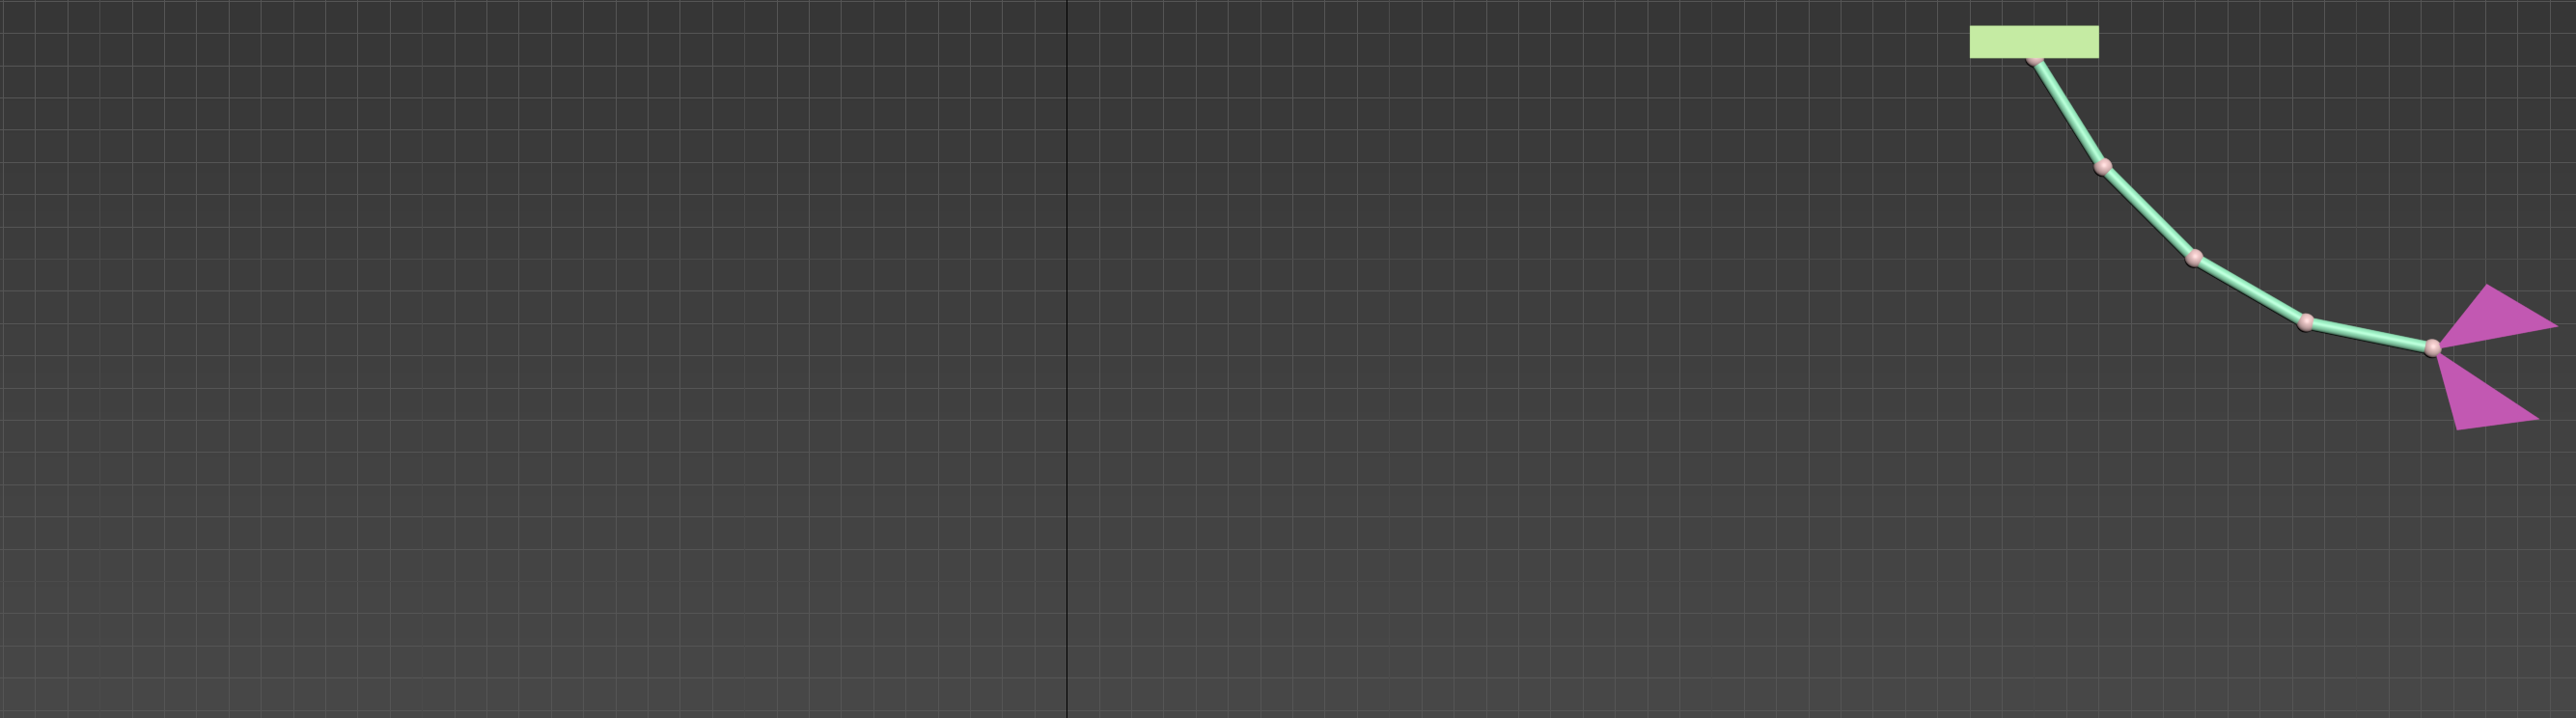
\includegraphics[width=\textwidth]{imagenes/Ejercicio4/keyframes/47.png}
    \caption{Rotación de los segmentos del brazo en el instante 47.}
\end{figure}

\begin{figure}[H]
    \centering
    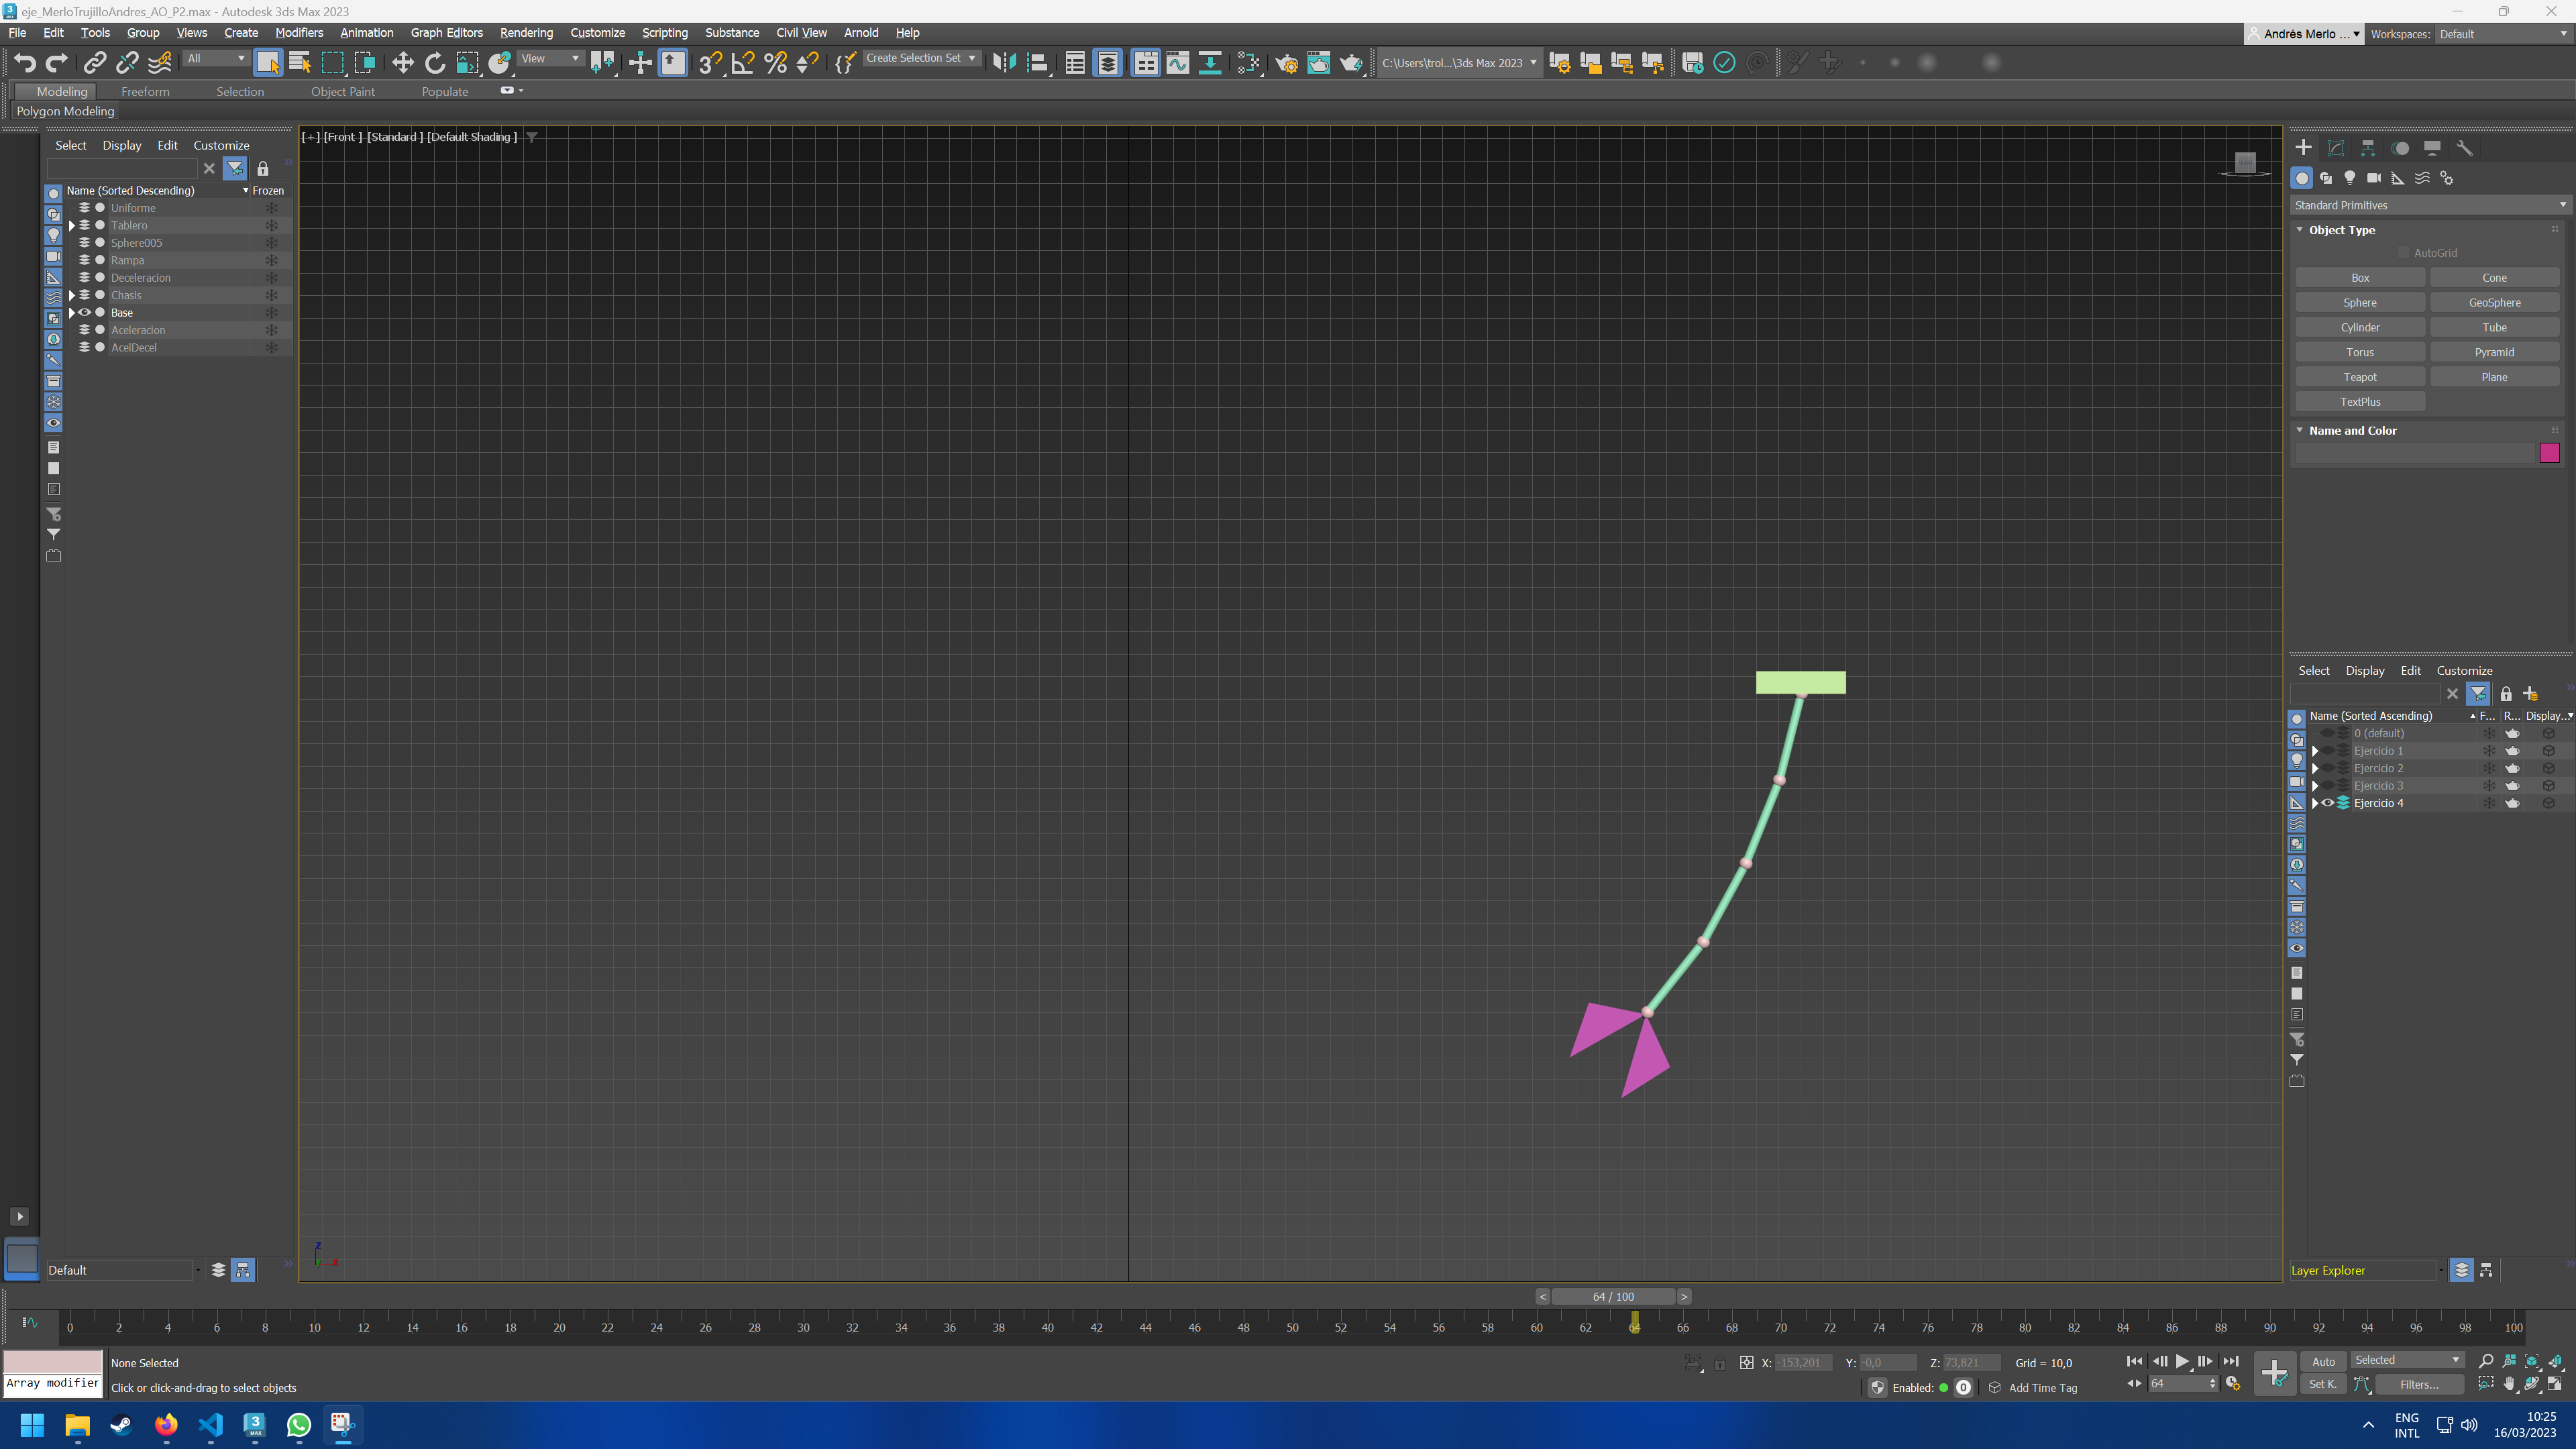
\includegraphics[width=\textwidth]{imagenes/Ejercicio4/keyframes/64.png}
    \caption{Rotación de los segmentos del brazo en el instante 64.}
\end{figure}


\begin{figure}[H]
    \centering
    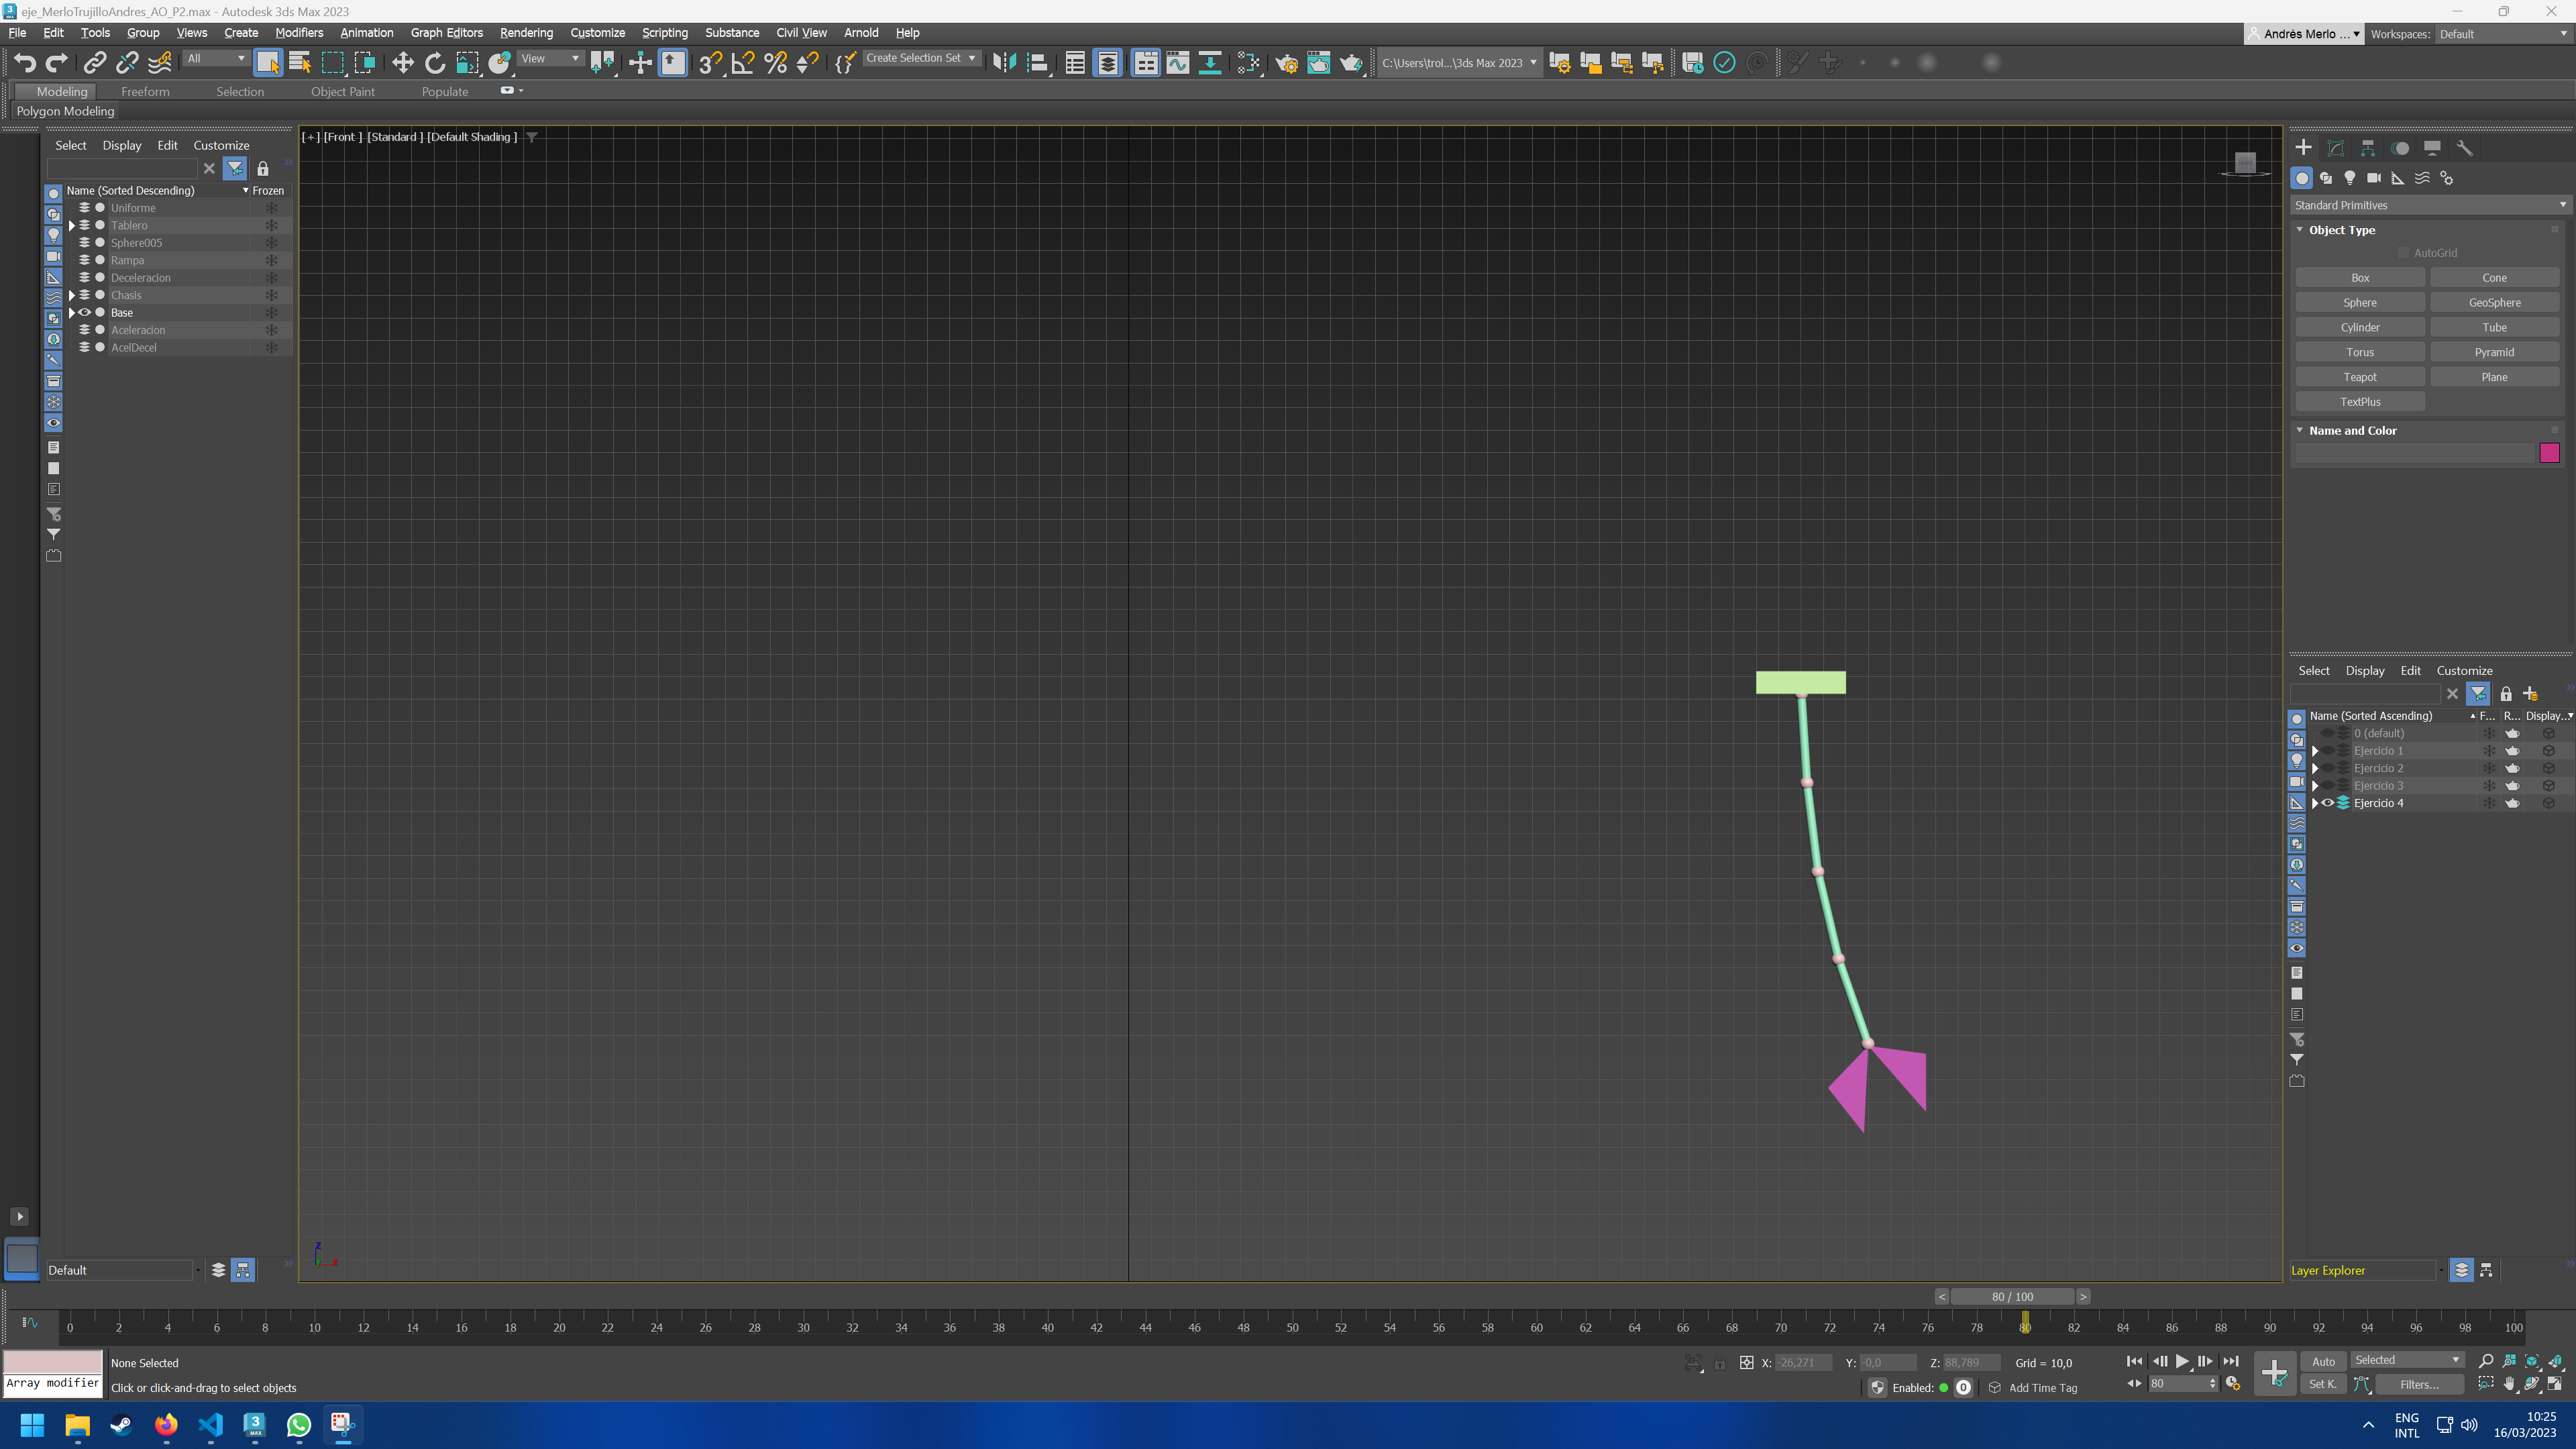
\includegraphics[width=\textwidth]{imagenes/Ejercicio4/keyframes/80.png}
    \caption{Rotación de los segmentos del brazo en el instante 80.}
\end{figure}

\begin{figure}[H]
    \centering
    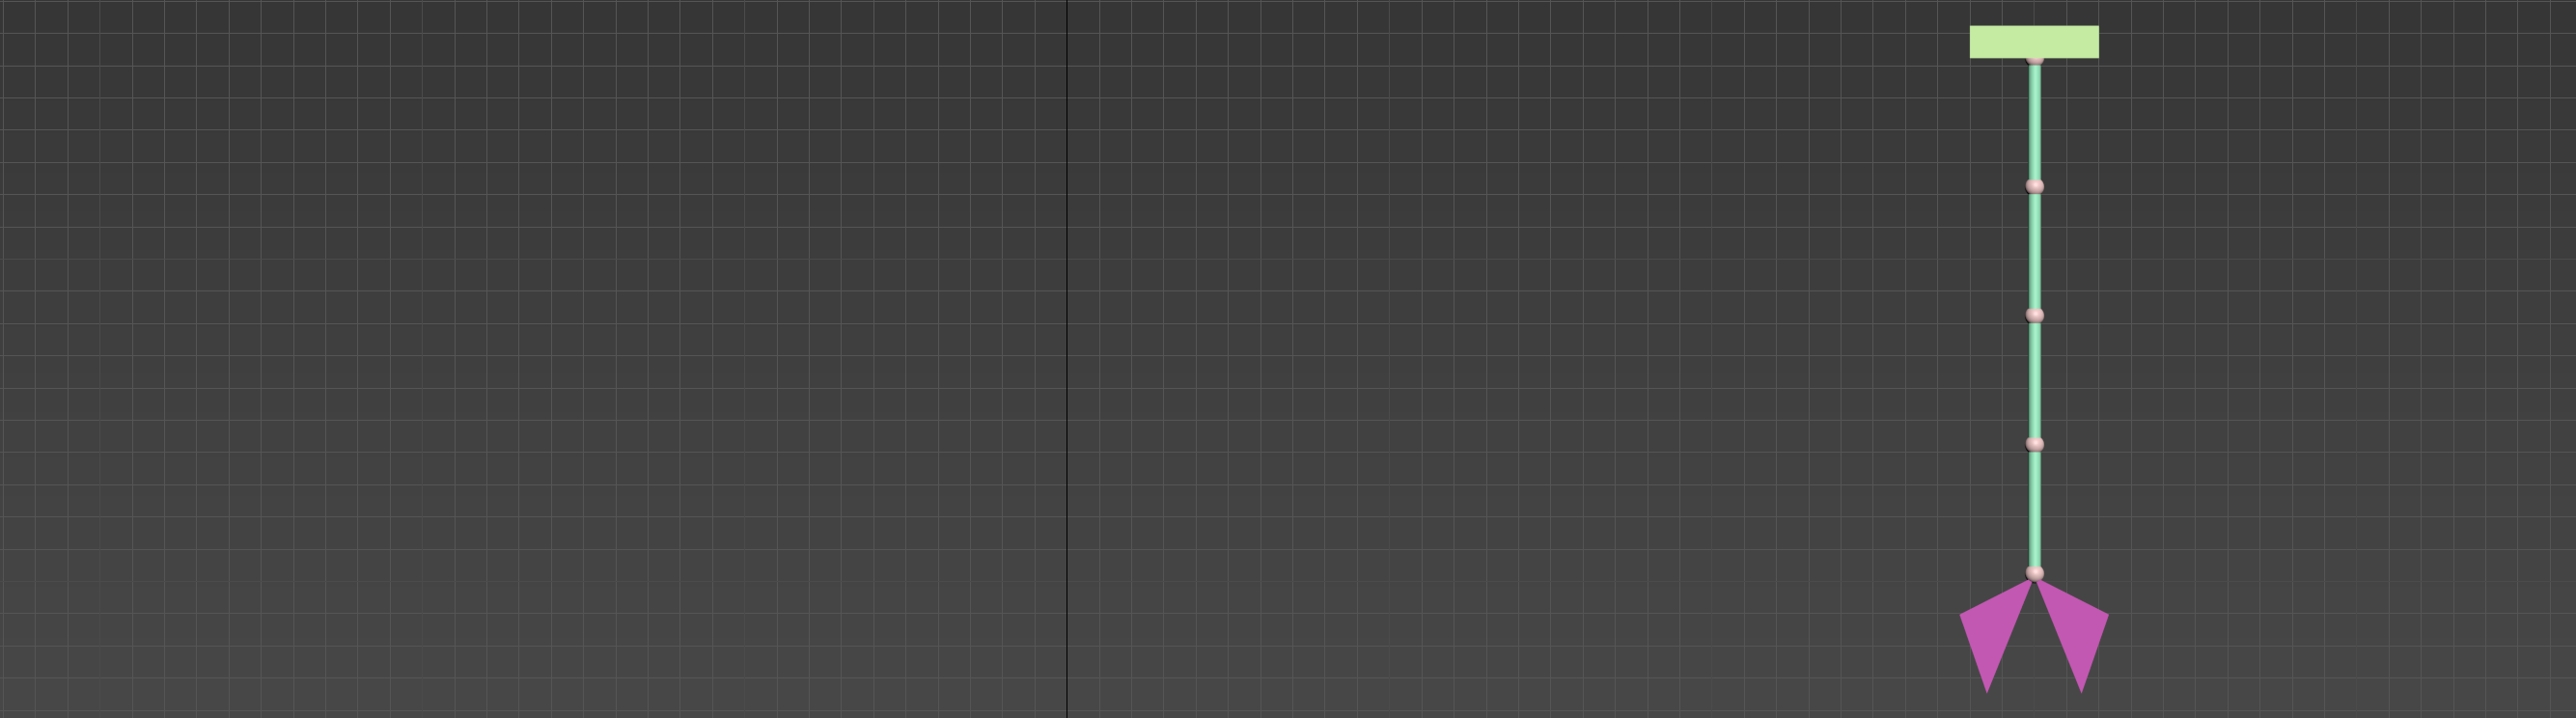
\includegraphics[width=\textwidth]{imagenes/Ejercicio4/keyframes/96.png}
    \caption{Rotación de los segmentos del brazo en el instante 96.}
\end{figure}

% explicar el significado del instante 18 (rescribir)
El instante 18 lo he puesto porque sin él la animación de rotar el brazo por la velocidad no se acababa hasta el punto en el que la plataforma parase, haciendo que la animación no quedase demasiado convincente. Haciendo esto, he conseguido que el brazo rote del todo antes de parar.

%curva
La curva para la aniamción de la plataforma es la siguiente:

%foto de la curva
\begin{figure}[H]
    \centering
    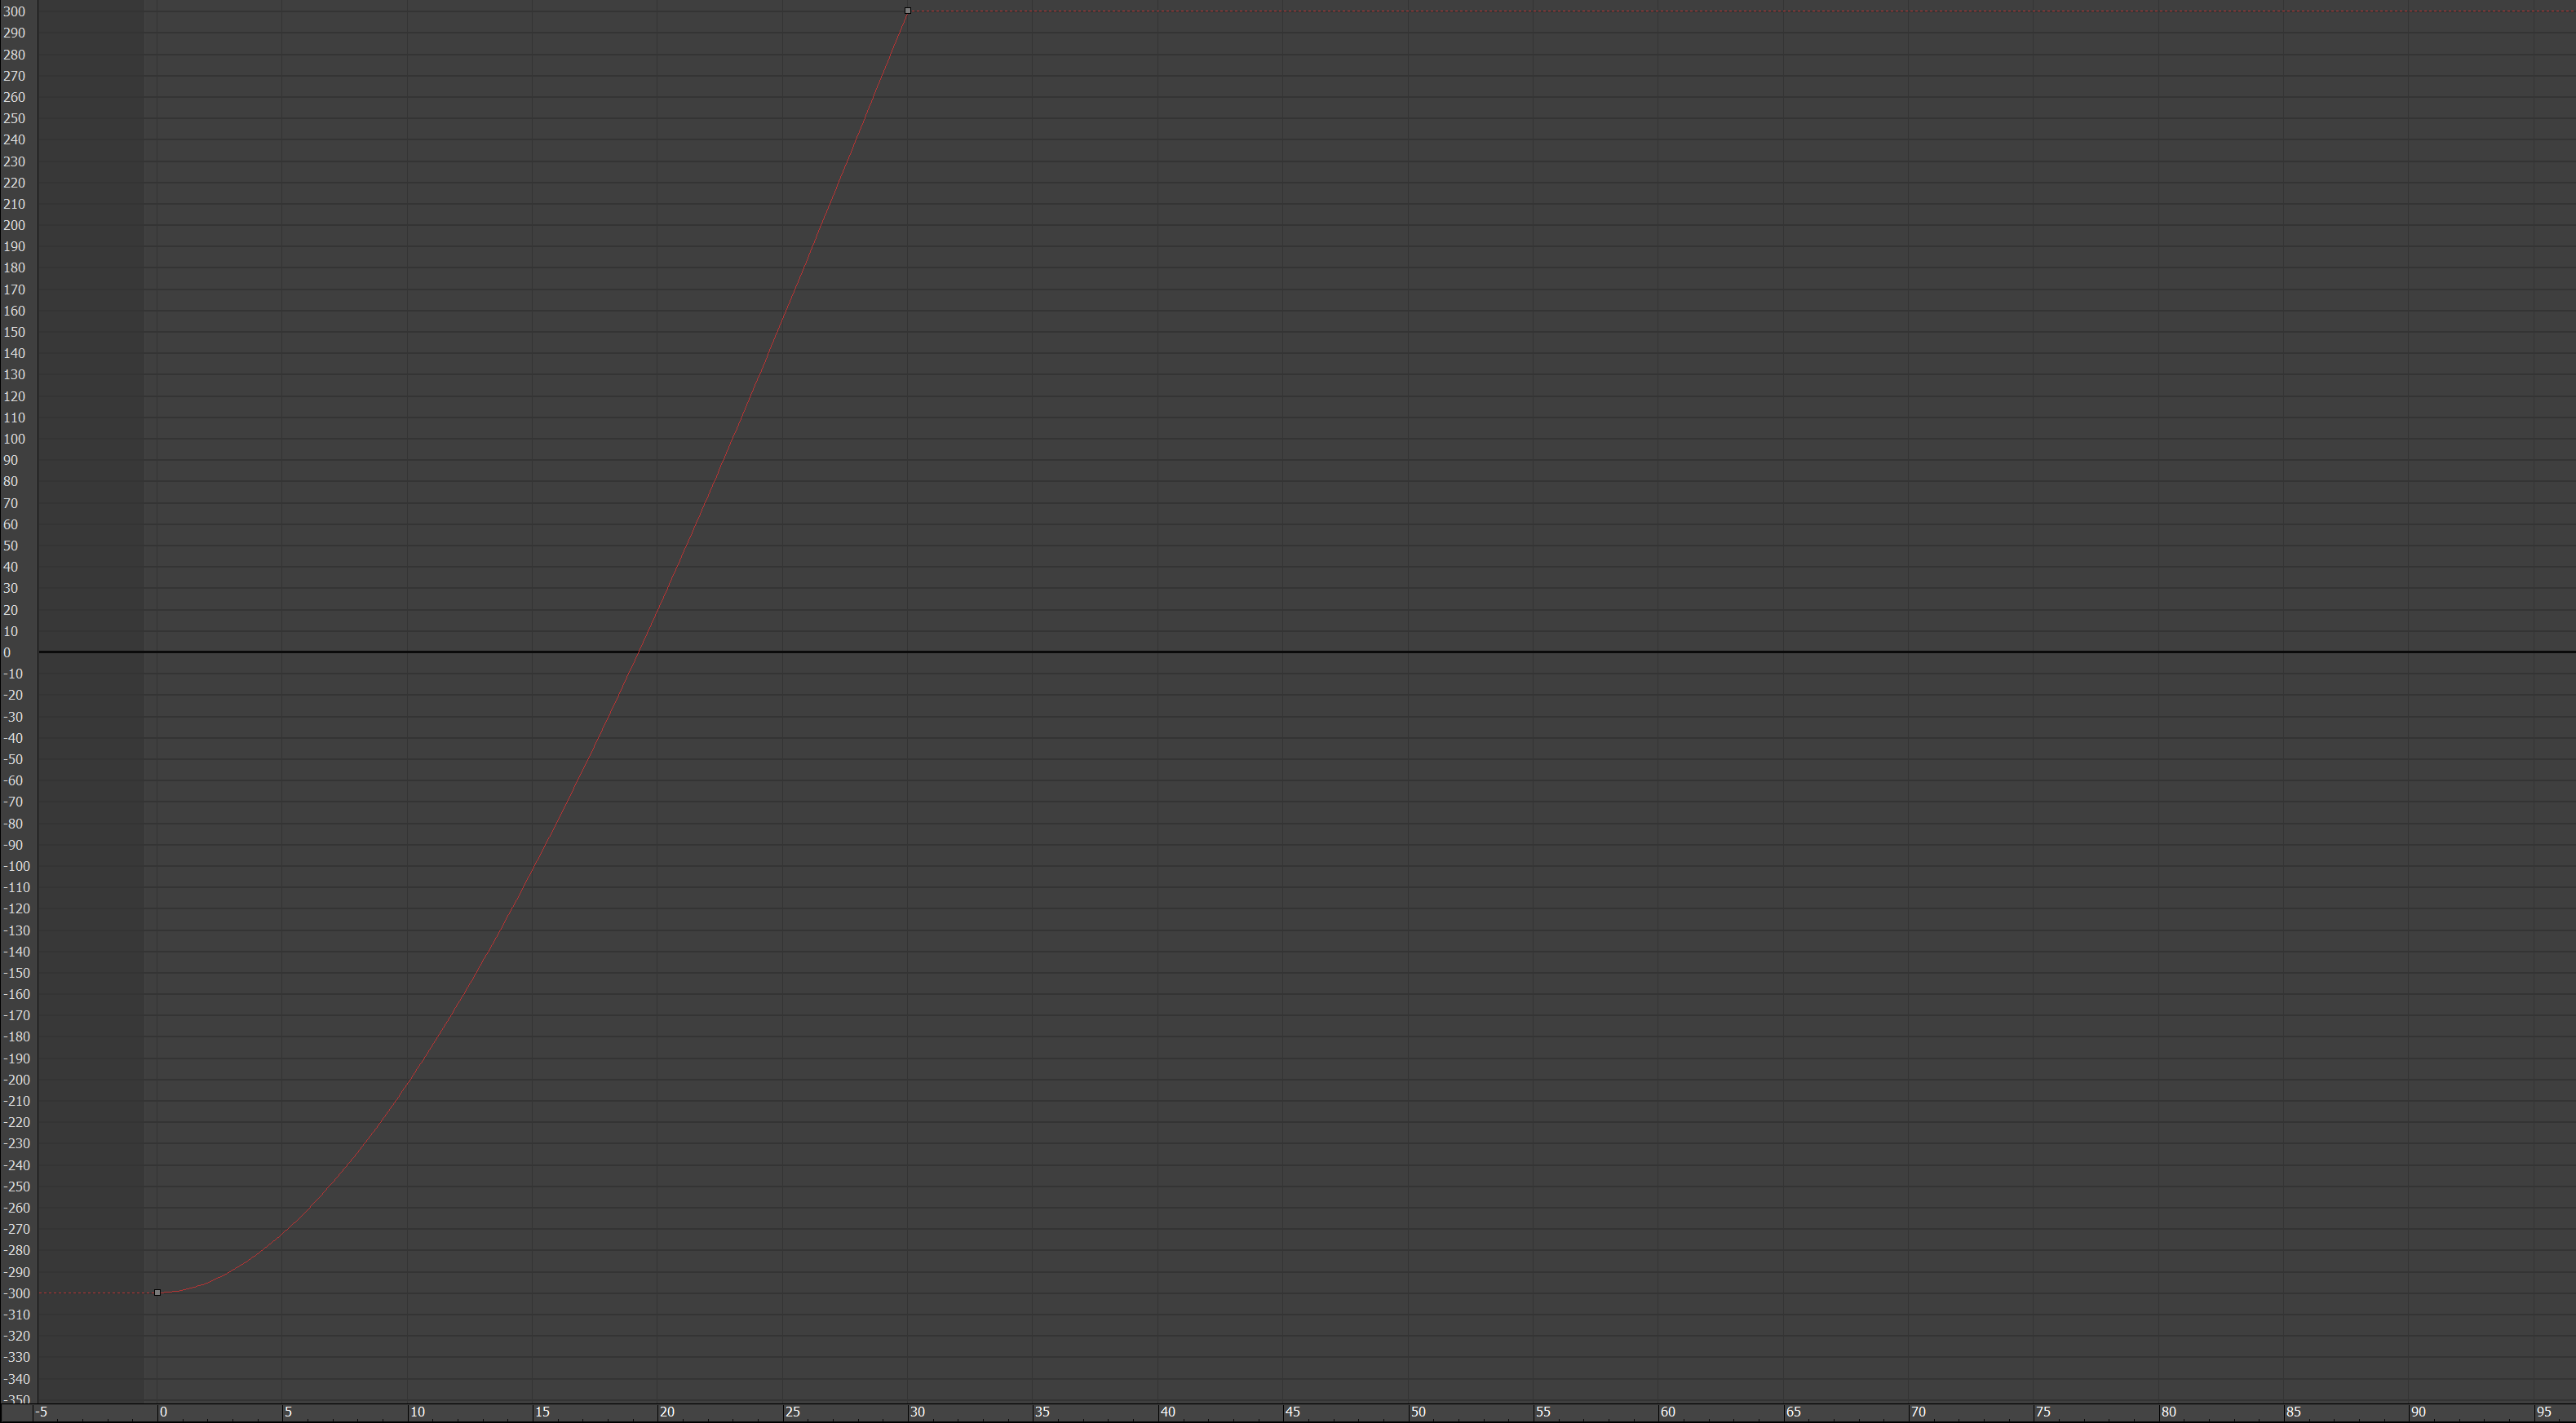
\includegraphics[width=\textwidth]{imagenes/Ejercicio4/curvas/base/red.png}
    \caption{Curva de la posición en el eje X de la plataforma con respecto al tiempo.}
\end{figure}


Dicha curva lo que hace es, al principio acelera y cuando llega al punto final se para bruscamente (mediante la curva lineal). Esto lo he hecho asi para que el latigazo que realiza el brazo sea mas realista, ya que si se va frenando progresivamente no queda del todo bien.

Las curvas de los segmentos del brazo son muy similares entre si, por lo que solo voy a mostrar uno.

%foto de la curva
\begin{figure}[H]
    \centering
    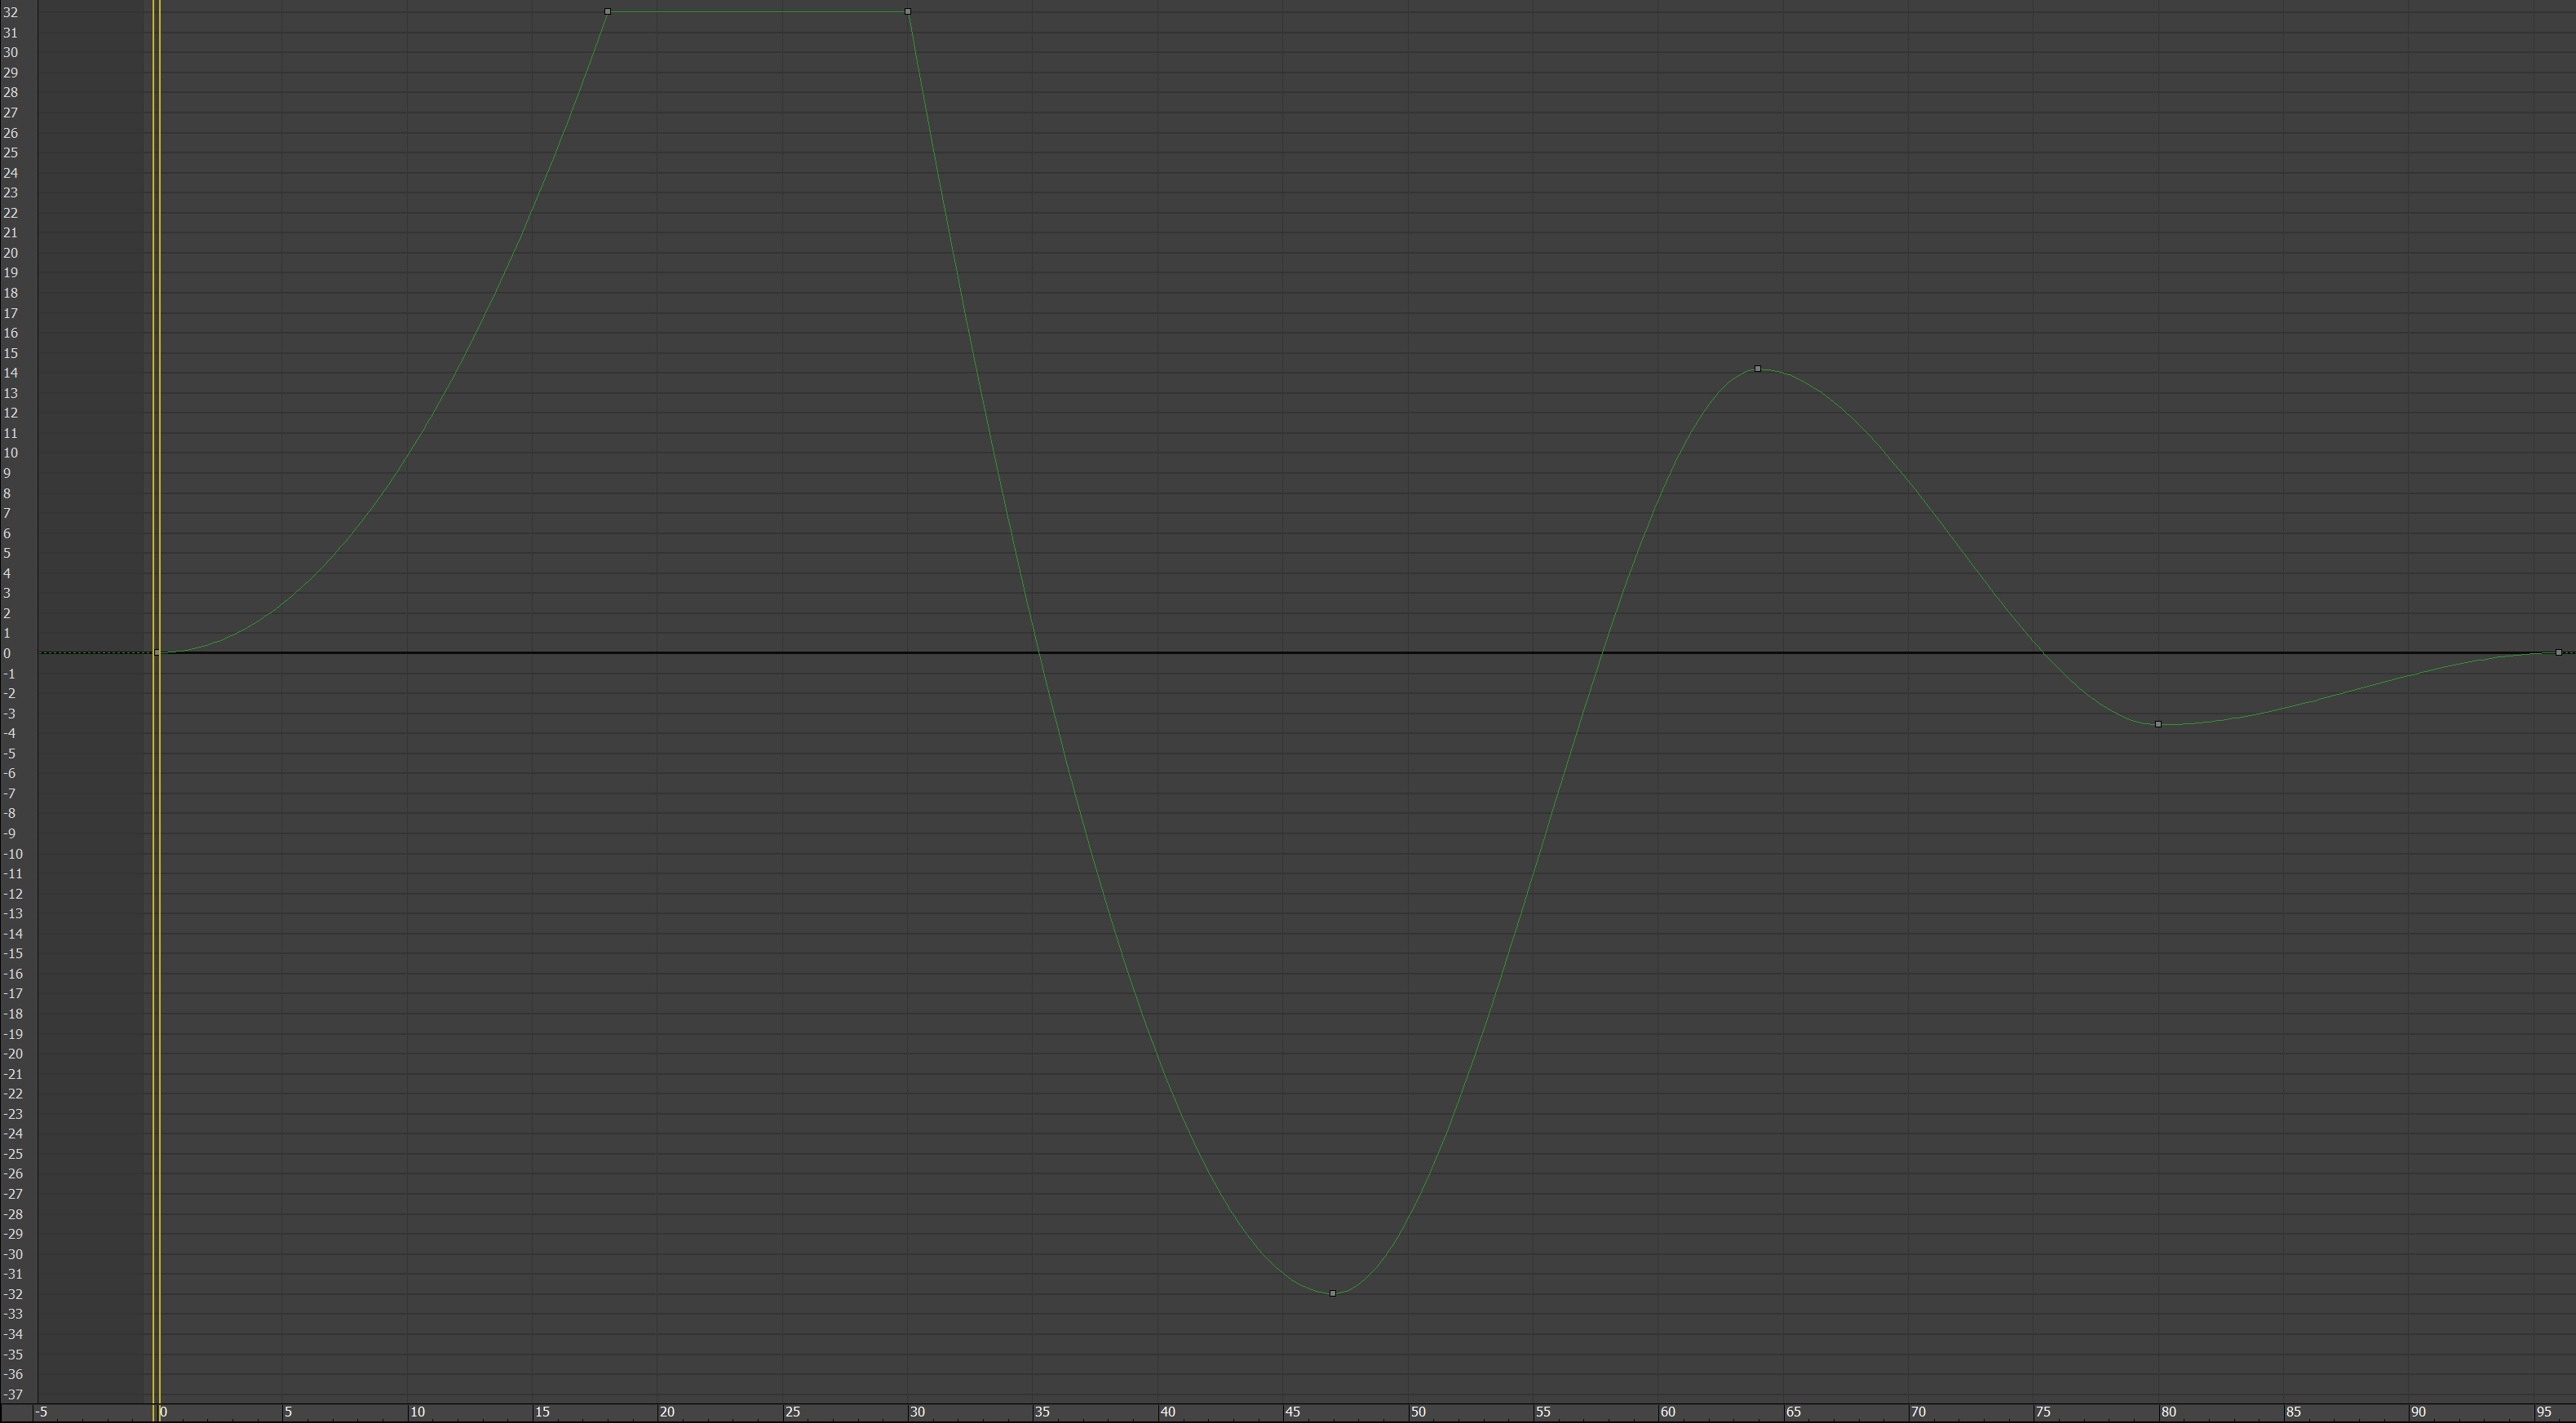
\includegraphics[width=\textwidth]{imagenes/Ejercicio4/curvas/segmentos/green.png}
    \caption{Curva de la rotación en el eje Y de los segmentos con respecto el tiempo.}
\end{figure}

%rescribir
Esta curva lo que hace es seguir la aceleracion de la plataforma al principio, hasta llegar al instante 18 que he hablado anteriormente, asi se consigue que el movimiento sea mas natural. Despues se mantiene constante al no requerir rotacion ninguna. Cuando la plataforma para, se sigue una curva de desaceleracion, ya que la energia que tenia la pataforma se transfiere al brazo. Finalmente, se utilizan curvas de aceleración, desaceleracion y \textit{Slow in/Slow out} (union de ambas) para simular el baiben que hace hasta parar por las distintas fuerzas.


\end{document}
